%%%%%%%%%%%%%%%%%%%%%%%%%%%%%%%%%%%%%%%%%%%%%%%%%%%%%%%%%%%%%%%%%%%%%%%%%%%
% filename    : sp.tex
% author      : 
%%%%%%%%%%%%%%%%%%%%%%%%%%%%%%%%%%%%%%%%%%%%%%%%%%%%%%%%%%%%%%%%%%%%%%%%%%%

% BUGFIX: Save LaTeX kernel version of \@xfloat
\makeatletter
\let\my@xfloat\@xfloat
\makeatother

% use ateneo de naga etd class (actually modified virginia tech's etd class)
\documentclass[oneside]{etd}

% BUGFIX: Create a modified copy of \@xfloat using the kernel definition
\makeatletter
\def\@xfloat#1[#2]{
	\my@xfloat#1[#2]%
	\def\baselinestretch{1}%
	\@normalsize \normalsize
}
\makeatother
\hbadness=10000
\hfuzz=5pt
\tolerance=1000
% use these packages
\usepackage{array}
\usepackage{graphicx}
\usepackage{amssymb}
\usepackage{gensymb}
\usepackage{latexsym}
\usepackage{amsmath}
%\usepackage[lineno5,noindent]{lgrind}
%\usepackage{rotating} 
%\usepackage{makeidx}
%\usepackage{stmaryrd}
\usepackage{float}
\usepackage{subfigure}
%\usepackage{cite}
%\usepackage{moreverb}
%\usepackage{pictexwd,dcpic}
\usepackage{algorithm,algorithmic}
\renewcommand{\algorithmicrequire}{\textbf{Input:}}
\renewcommand{\algorithmicensure}{\textbf{Output:}}
\usepackage{tikz}
\usetikzlibrary{positioning,calc}

\usepackage{listings}
\definecolor{cppred}{rgb}{0.6,0,0} % for strings
\definecolor{cppgreen}{rgb}{0.25,0.5,0.35} % comments
\definecolor{cpppurple}{rgb}{0.5,0,0.35} % keywords
\definecolor{cppdocblue}{rgb}{0.25,0.35,0.75} % doc
 
\lstset{language=C++,
basicstyle=\linespread{0.8}\ttfamily\small,
keywordstyle=\color{cpppurple}\bfseries,
stringstyle=\color{cppred},
commentstyle=\color{cppgreen},
morecomment=[s][\color{cppdocblue}]{/**}{*/},
numbers=left,
numberstyle=\tiny\color{black},
% stepnumber=2,
numbersep=10pt,
tabsize=4,
showspaces=false,
showstringspaces=false}

\graphicspath{{figures/}{./}}

%\renewcommand{\floatpagefraction}{0.8}

\setcounter{secnumdepth}{3}
\setcounter{tocdepth}{3}

\makeindex

%%%%%%%%%%%%%%%%%%%%%%%%%%%%%%%%%%%%%%%%%%%%%%%%%%%%%%%%%%%%%%%%%%%%%%%%%%%

\title{KABISIG: A Web-Based Kabataan Information System for Inclusive Governance}
\department{Computer Science}
\BSthesis % options: \BSthesis \BSproject \BShonors \Mdegree \MSdegree \PhDdegree
\degreemonth{5 October}  % date of final defense
\degreeyear{2026}

\twostudents % options: \onestudent \twostudents 
{David James B. Ignacio}
{Ashley Kyla D. Vinzon}

\studentsheader
{Ignacio, Vinzon}

\twodegrees % options: \onedegree \twodegrees 
{Information Technology}
{Information Technology}


\advisor
{Lowie Vincent S. Bisana}
\threemembers
{Kurt Gilbert D. Tapel}
{Paul Angelo S. Silvestre}
{Jelly P.Aureus}
\deanandchair
{Marianne Ang-Tolentino}
{Jelly P.Aureus}

\keywords{Sangguniang Kabataan, Program and Participant Tracking, Barangay Youth Council Information System, Multi-Tenancy, Inclusive Governance, E-Governance, Naga City}
\makeatletter
\def\thebibliography#1{\chapter*{REFERENCES\@mkboth
 {REFERENCES}{REFERENCES}}\singlespace\list
 {[\arabic{enumi}]}{\settowidth\labelwidth{[#1]}\leftmargin\labelwidth
 \advance\leftmargin\labelsep
 \usecounter{enumi}}
 \def\newblock{\hskip .11em plus .33em minus .07em}
 \sloppy\clubpenalty4000\widowpenalty4000
 \sfcode`\.=1000\relax}
\def\endthebibliography{\endlist\endsinglespace}
\makeatother

\begin{document}
\nocite{A,B,C,D,E,F,G,H,I,J,K,L,M,N,O,P,Q,R,S,T,U,V,W,X,Y,Z,
        AA,AB,AC,AD,AE,AF,AG,AH,AI,AJ,AK,AL,AM,AN,AO,AP,AQ,AR,AS,AT,
        AU,AV,AW,AX,AY,AZ,BA,BB,BC}
%edit etd.cls to accommodate lesser number of proponents
\maketitle
\makerecomm
\makeacceptance
\makedeclaration

%%%%%%%%%%%%%%%%%%%%%%%%%%%%%%%%%%%%%%%%%%%%%%%%%%%%%%%%%%%%%%%%%%%%%%%%%%%
%                    ABSTRACT/EXECUTIVE SUMMARY                           %
%%%%%%%%%%%%%%%%%%%%%%%%%%%%%%%%%%%%%%%%%%%%%%%%%%%%%%%%%%%%%%%%%%%%%%%%%%%

% can use execsummary or abstract
\begin{abstract}
	\hspace*{\parindent}In the existing situation, the SK councils in Naga City use manual and semi-digital methods in recording their activities that involve youth programs, such as participant information, cost, and other relevant data. The said methods had led to poor documentation, delays in reporting, difficulties in monitoring, and non-transparency. To solve the aforementioned problems, the current project came up with a multi-tenant web-based Kabataan Information System called KABISIG (Kabataang Bagong Sistema para sa Inklusibong Gobyerno).\vspace{5mm} 
    
    \hspace*{\parindent}Through KABISIG, SKs can now fully capture youth information and streamline automation of registration and attendance with the ability to perform analytics on this data in real time. SKs can also use the system to improve their programs by continuously adding features such as civic feedback (Boses ng Kabataan), resolution tracking, youth polling (which can be done anonymously), and cross-barangay federation analytics, among others. The system is designed using a framework of Next.js, React, TypeScript, TailwindCSS, and Supabase (PostgreSQL) and incorporates a web-based, three-tier system and Agile Scrum Methodology. The system encompasses seven user roles under five stakeholder tiers: Super Administrator, Barangay Administrator (SK Chairperson), SK Official, Youth Constituent, Viewer, Federation Observer, and LGU Auditor. This platform offers a multi-tenant solution for the various Sangguniang Kabataan councils in Naga City. This provides an infrastructure to allow each barangay to manage its own records.\vspace{5mm}
    
    \hspace*{\parindent}This solution provides benefits for each barangay SK council in the city, and offers e-governance at the barangay level for youth management.\vspace{5mm}
\end{abstract}

\begin{dedication}

\hspace*{\parindent}We dedicate this work to all the youth and SK officials who strive for better governance, and to our families who supported us throughout this journey.

\end{dedication}


\begin{acknowledgements}

\hspace*{\parindent}We thank our project advisor, Lowie Vincent S. Bisana, for his guidance and support. We extend our gratitude to the SK officials and youth participants of Barangays in Naga City for their valuable time and feedback during the requirements gathering and evaluation phases. We also acknowledge the panel members whose recommendations significantly shaped the evolution of this project into the finalized KABISIG platform. \vspace{5mm}


\end{acknowledgements}


\begingroup
\renewcommand*{\addvspace}[1]{}
\tableofcontents
\listoffigures
\listoftables
\endgroup

\beginbody
\pagenumbering{arabic}

%%%%%%%%%%%%%%%%%%%%%%%%%%%%%%%%%%%%%%%%%%%%%%%%%%%%%%%%%%%%%%%%%%%%%%%%%%%
\chapter{Introduction}
%%%%%%%%%%%%%%%%%%%%%%%%%%%%%%%%%%%%%%%%%%%%%%%%%%%%%%%%%%%%%%%%%%%%%%%%%%%

\section{Project Context}

\hspace*{\parindent}The SK program in the Philippines was conceived with the community being its primary foundation. The creation of the program was a consequence of advocacy meant to promote learning among the youth about governance and their involvement in it. The SK operates under the provisions of the Local Government Code of 1991 and the Sangguniang Kabataan Reform Act of 2015 (RA 10742) \cite{AV}. Both the acts state that the SK has a role in the design and implementation of youth programs and the opportunity for practicing governance and leadership \cite{AV}. It is the responsibility of the SK members to identify interests of the youth, implement programs and projects and manage finances associated with the programs/projects. The autonomy of the SK has been further increased through RA 11768 (2022) \cite{AW} allowing the organization to carry out youth programs.
\vspace{5mm}

\hspace*{\parindent}There are multiple challenges affecting the implementation of the legal mandates of the SK. They include low youth participation, shortage of financing, inadequacies in recording and monitoring the programs, as well as the discrepancy between the planned and actual activities \cite{J,I,L,AS}. The information management system needed by the councils to enable transparency and community participation, as well as the effective monitoring of programs, is often absent \cite{AE,AG,AH}.
\vspace{5mm}

\hspace*{\parindent}The SK councils in Naga City keep records in the form of files and take down attendance and participation data using spreadsheets. Announcements are made through social media such as Facebook and Messenger. However, in Naga City, the SK councils need to gather photographs and activity reports, print files and documents and prepare reports for the Barangay and City offices. Therefore, report writing is time consuming and monitoring of the participation of the youth poses a challenge. The absence of files and incompleteness of records represent additional challenges. Additionally, there are no resources for conducting program evaluations and making data-driven decisions; moreover, the councils have difficulties monitoring and improving their programs. Even though the number of youths participating in various activities in Naga City is considerable, the councils use semi-digital methods for handling them. Thus, identifying program beneficiaries, evaluating activities results and reporting on activities remains problematic. The management, monitoring and reporting on programs of the SK councils in Naga City would greatly benefit from the introduction of the web-based information system based on the community information systems used in other communities.
\vspace{5mm}

\hspace*{\parindent}The solution to these problems is sought through KABISIG --- a multi-tenant, web-based Kabataan Information System designed for Sangguniang Kabataan Councils in the City of Naga, which helps with the management and monitoring of the youth programs' participants, financial asset oversight and youth participation promotion, thus addressing former problems.
\vspace{5mm}

\section{Purpose and Description}

\hspace*{\parindent}The purpose of this project is to develop, test and improve an online Kabataan Information System which will serve to enhance the operational effectiveness, efficiency and transparency of SK activities in Naga City. This purpose is in line with the principle of good governance as transparency, accountability, participation and efficiency in public service delivery. As a result of this project KABISIG is developed --- a flexible platform scalable and adjustable for all SK councils in Naga City.
\vspace{5mm}

\hspace*{\parindent}KABISIG solves the problems of insufficient reporting, delayed reporting and inconsistencies in the operations which were present in former applications by combining manual and digital process in one application. Program management, participant tracking, budget transparency and analytical tools for civic engagement and governance are combined in one platform. Being constituted as a multi-tenant system KABISIG provides Sangguniang Kabataan councils in Naga City with the opportunity to manage their data using the same infrastructure.
\vspace{5mm}

\section{Objectives}

\subsection{Main Objective}

\hspace*{\parindent}This project involves the design, development, and implementation of a standardized, cloud-based, multi-tenant information system for all SK councils in Naga City. The proposed system is intended to automate and streamline essential governance processes, including resident profiling and participant management, program scheduling and online registration, attendance monitoring through QR-based validation, financial and budget control, document and records management, reporting and analytics, citizen feedback collection and analysis, resolution tracking, notification handling, and social media integration. By integrating these modules, the system ensures maximum usability and high user satisfaction in compliance with ISO 25010 quality standards and the Technology Acceptance Model (TAM). Furthermore, the architecture is designed to deliver reliable performance in terms of processing time, accuracy, and data availability, while maintaining strict data segregation at the barangay level to enhance security, scalability, and administrative efficiency.
\vspace{5mm}

\subsection{Specific Objectives}

\begin{itemize}
    \item To identify the constraints of the existing SK program and participant management system in Naga City.
    \item To develop a standardized, cloud-based, multi-tenant system for all SK councils in Naga City.
    \item To design and develop the following system modules:
    \begin{itemize}
        \item Resident Profiling and Participant Management
        \item Program Scheduling and Online Registration
        \item Attendance Monitoring
        \item Budget Control
        \item Document and Records Management
        \item Reporting and Citizen Feedback
        \item Resolution Tracking
        \item Notification Handling
        \item Social Media Integration (Facebook Synchronization)
    \end{itemize}
    \item To evaluate the perceived satisfaction and usability of the system among SK officials and youth participants using ISO 25010 and TAM.
    \item To evaluate the performance of the system in terms of processing time, accuracy, and data availability.
\end{itemize}
\vspace{5mm}

\section{Scope and Limitations}

\subsection{Scope}

\hspace*{\parindent}The goal of the project is to create a Web-Based Kabataan Information System called KABISIG designed to cater to the requirements of every SK in all the barangays of Naga City. The main purpose of the KABISIG is to establish a single system through which the SK officials can carry out their tasks efficiently. The tasks involved include: profiling of youths in the barangay, management of SK programs and activities, beneficiary monitoring per program or activity, budget and expense tracking per program or activity, keeping of necessary documents for the effective running of SK, encouragement of youths to give feedback on the activities of the government, and report generation for monitoring purposes. The system will also provide SK officials dashboards and analytics for deriving easy conclusions from the collected data. The architecture of KABISIG is multi-tenant making it possible for each barangay to create its private and secure accounts away from others. It is also web-based and mobile responsive.
\vspace{5mm}

\subsection{Limitations}

\hspace*{\parindent}While KABISIG provides a comprehensive platform for automating and streamlining SK council operations, the system has certain limitations in scope and capability:
\vspace{5mm}

\begin{itemize}
    \item \textbf{Intelligent Features:} All ``automated'' features are rule-based and use simple if-then logic or keyword matching. The system does not implement true AI, machine learning, deep learning, or natural language processing (NLP) models.
    \item \textbf{No AI Decision-Making:} The system does not incorporate artificial intelligence for decision-making, prediction, or recommendation.
    \item \textbf{External Integrations:} Integration with external government databases such as DILG, PSA, BIR, COA, and DBM is beyond the scope of this project.
    \item \textbf{Hardware-Based Functions:} Functions associated with hardware such as biometric recognition and QR code scanners are excluded. QR codes are generated and scanned through the device's camera using WebRTC and Web Barcode Detection API.
    \item \textbf{SMS and Social Media:} SMS gateway capabilities are not included. Facebook integration is limited to basic posting via the Meta Graph API.
    \item \textbf{Reporting:} Evaluation of programs and activities in the system depends only on the information available in the system.
    \item \textbf{Offline Capability:} The system requires an internet connection. Offline functionality is not supported.
\end{itemize}
\vspace{5mm}

\section{Significance of the Study}

\hspace*{\parindent}This project benefits multiple stakeholders within Naga City:
\vspace{5mm}

\begin{itemize}
    \item \textbf{SK Officials:} Benefit from the decrease in the manual workload by 80\% as well as the provision of real-time compliance reports and data-driven decision-making. The reduction in the SK workload is expected to improve efficiency and effectiveness of SK operations in line with the results of research on digital governance of local government units. The adopted technology facilitates program management, participant tracking, financial accounting, and governance documentation that enables SK officials to spend less time on administrative tasks and more time providing youth services.

    \item \textbf{Youths:} Enjoy easy online registration, budget transparency, and means to participate in local governance through the provision of feedback and digital Youth IDs. The youth participation initiative called Boses ng Kabataan gives opportunities for youths to contribute to the process of governance by presenting ideas and expressing concerns regarding programs and resolutions within the local youth council.

    \item \textbf{SK Federations:} Gain cross-barangay analytics used in the planning of the Local Youth Development Plan (LYDP). Federation-level governance oversight tools allow the SK Federation President to evaluate the performance of governance in barangays, compare participation rates and demographics, budget allocations, and generate reports at the federation level.

    \item \textbf{Local Government Units (LGUs):} Obtain centralized information on youth population for evidence-based planning and transparency. Public access to compliance reports and budget summaries improves SK activity oversight.

    \item \textbf{Barangay Management:} Can apply KABISIG beyond SK operations by modifying existing modules for barangay administration purposes such as resident profiling, program and event management, document management, public announcements, community engagement, and organization monitoring. The flexibility of the design supports future barangay digitalization projects without limiting them only to youth governance.

    \item \textbf{Communities:} Benefit from increased accountability and inclusiveness in governance due to KABISIG's implementation. Public dashboards provide transparency, participation, accountability, and effectiveness, aligning with good governance principles and United Nations Sustainable Development Goal 16 on building effective, accountable, and inclusive institutions.

    \item \textbf{Academe:} The project can be used as an example in relation to the field of e-governance in the local government setting, especially youth governance. The project is a replicable framework for another local government unit that intends to automate its youth council operations using multi-tenant architectures in the Philippines' Barangay setting. The project contributes to the growing body of literature on e-governance in the Philippines \cite{C,D,V,AM} and multi-tenant architectures in public services delivery \cite{AS}.

    \item \textbf{Future Researchers:} Can use this study as a resource material in building and improving information systems in local governance, e-government, youth development, and public administration. The design, features, intelligent analytics, and multi-tenant deployment of the system provide a base for further studies on decision support systems, digital governance solutions, engagement technologies, and advanced technologies like artificial intelligence and predictive analytics in local government environments.
\end{itemize}
\vspace{5mm}
%%%%%%%%%%%%%%%%%%%%%%%%%%%%%%%%%%%%%%%%%%%%%%%%%%%%%%%%%%%%%%%%%%%%%%%%%%%
\chapter{Review of Related Systems and Literature}
%%%%%%%%%%%%%%%%%%%%%%%%%%%%%%%%%%%%%%%%%%%%%%%%%%%%%%%%%%%%%%%%%%%%%%%%%%%

\hspace*{\parindent}This chapter gives a review and synthesis of the relevant studies on the development of the online SK information system as discussed in the KABISIG paper. It covers the legal and institutional framework of the SK system, youth participation in local governance, good governance, digital transformation in barangay governance, existing information systems of the SK, and technical aspects of the proposed system such as multi-tenancy, information systems, and system evaluation. This chapter ends with the synthesis of the literature and the research gap of the study.
\vspace{5mm}

\section{Theoretical and Conceptual Background}

\subsection{The Sangguniang Kabataan in Philippine Governance}

\hspace*{\parindent}The Sangguniang Kabataan (SK) system is the lowest administrative unit and deals with the concerns of the youth with regard to the implementation of youth projects and programs of the government. The legal framework of the SK system is Republic Act No. 10742 which is known as the Sangguniang Kabataan Reform Act of 2015 \cite{AU}. Through this law, SK councils gain autonomy in financial transactions by allocating 10\% from the general funds of the barangay for the formulation of the Comprehensive Barangay Youth Development Plan (CBYDP) and the Annual Barangay Youth Investment Program (ABYIP) \cite{AV}.
\vspace{5mm}

\hspace*{\parindent}Republic Act No. 11768 institutionalized reforms to revitalize youth participation in the local governance process \cite{AV}. It enhances the capacity of the SKs by giving honorarium and other forms of incentive to SK officials and by amending certain provisions of RA 10742. The Revised Implementing Rules and Regulations of RA 10742 as amended by RA 11768 covers the operational aspects of the SK system such as holding of Katipunan ng Kabataan (KK) assemblies, budget planning and compliance among others \cite{N}.
\vspace{5mm}

\hspace*{\parindent}In academic literature, there are discussions on the development of the SK system and how it would affect Republic Act 10742 with respect to youth participation and capability considerations as well as arguments for the reform of the SK system \cite{S}. Results of the national survey conducted five years after the implementation of the Sangguniang Kabataan Reform Law show improvement in the political and participatory governance framework but still some issues on legislation, financial management and compliance especially on the Local Youth Development Plans remain \cite{T}.
\vspace{5mm}

\hspace*{\parindent}There are many guidelines established through the issuance of the memorandum circulars of the Department of Interior and Local Government (DILG). In the case of the operations of SK, one such example would be the Memorandum Circular No. 2022-033 on the profiling of the Katipunan ng Kabataan and establishment, maintenance, updating, and submission of youth database \cite{L}. It is relevant to mention that this circular provides support to the Youth Profiling and Beneficiary Management module within KABISIG. Still, it should be noted that collecting and keeping data about youths should be done while respecting the right to privacy provided by the Constitution and the Data Privacy Act of 2012 \cite{AT}, which obliges the government to collect personal information only for legitimate purposes and with the consent of the data subjects. National Privacy Commission (NPC) has published guidelines (NPC Circular No. 2022-04) \cite{AH} on that matter and requires the designation of Data Protection Officers and the registration of data processing systems. Furthermore, there is NPC Advisory No. 2021-01 \cite{AG} with regard to the rights of the data subjects that ensures that youths are aware of their rights concerning personal data. All these measures make sure that the youth profiling activities carried out by KABISIG are done respecting privacy rights but still ensuring efficient program management and beneficiary targeting. Moreover, it is relevant to mention that NPC has commended the DILG for issuing issuances that contribute to the improvement of data privacy compliance among the LGUs \cite{AJ}. In turn, the Memorandum Circular No. 2023-068 establishes SK Full Public Disclosure (FPD) Policy, requiring SK documents, budgets, transactions, and plans to be disclosed \cite{M}. It is also useful for the implementation of the KABISIG's FPD Board and financial transparency portal.
\vspace{5mm}

\hspace*{\parindent}The empirical studies dealing with the operations of SK in certain localities, such as Lanao del Sur and Baguio City, prove that SK members take part in and help with various education, peacekeeping, and livelihood programs in those places \cite{AC,AN}. But at the same time, they face challenges while planning, documenting, and cooperating with the barangay government and other organizations \cite{AC,AN}. Thus, from the mentioned studies, it can be seen that SK is a valuable governance institution but with low capacity \cite{I,J,K}. Therefore, it is essential to pay attention to governance and planning framework development.
\vspace{5mm}

\subsection{Katipunan ng Kabataan Profiling and Data Collection Requirements}

\hspace*{\parindent}The collection of data related to youth under KABISIG is grounded in the regulatory framework developed by the Department of the Interior and Local Government (DILG) and the National Youth Commission (NYC). According to DILG Memorandum Circular No. 2022-033, KK Profiling must be conducted in order to ensure that each SK council has the capability to create and maintain the database of its youth \cite{L}.
\vspace{5mm}

\hspace*{\parindent}KK Profiling refers to the process of collecting demographical and personal information from youth who are between 15 and 30 years old according to Republic Act No. 10742 (Sangguniang Kabataan Reform Act of 2015) \cite{AU}. Personal data include such information as full name, gender, birthdate, age, contacts, address, educational history, among others. More specifically, the data fields that should be collected are determined in the KK Youth Profile Form (Annex 4 of DILG MC 2022-033) that serves as a standardized form for youth profiling activities \cite{L}.
\vspace{5mm}

\hspace*{\parindent}There are three primary reasons why data should be collected. They are: (1) provision of an up-to-date national database of Katipunan ng Kabataan members managed by the National Youth Commission; (2) provision of the ability to develop data-driven programs, projects, and legislations for SK councils based on the needs of their youth; (3) meeting DILG monitoring and reporting requirements \cite{L,AU}.
\vspace{5mm}

\hspace*{\parindent}Under Republic Act No. 10173, Data Privacy Act of 2012, all personal information must be handled confidentially and used only for its primary purpose \cite{AT}. In order to collect personal information, SK councils have to get an informed consent of data subjects that should be freely provided, specific, and informed. The National Privacy Commission (NPC) has introduced such guidelines as NPC Circular No. 2022-04 in which requirements to designate Data Protection Officers and register data processing systems were described \cite{AH}. There was also issued NPC Advisory No. 2021-01 that provided the detailed guidance on data subject rights \cite{AG}.
\vspace{5mm}

\hspace*{\parindent}It is important to highlight how KABISIG is consistent with the requirements above as the system allows for conducting KK Profiling through the digital platform that ensures the accuracy, security, and availability of the data. Moreover, KABISIG complies with data privacy regulations as it captures the data fields mandated by DILG MC 2022-033.
\vspace{5mm}

\subsection{Youth Participation, Political Socialization, and Digital Citizenship}

\hspace*{\parindent}Participation of young people in the SK scheme brings about several developmental benefits for each individual, including practical implementation of SK programs in the community. Empirical evidence points out that significant youth participation exists in educational, citizenship, governance, and health spheres. Each sphere contributes to the development of cognitive, social, civic, physical competencies, and leadership skills that include decision making and teamwork \cite{I}. Furthermore, there is a lot of empirical information about the impact of the SK program on a great number of Filipino youths if the program is organized according to the youth perspective \cite{G}. It is in compliance with the principle of participatory governance and the commitment of the Philippine government to real youth participation in decision making process. Though the SK program has proved its ability to develop problem solving, leadership and self-confidence skills among youth, the accent on digital flexibility and skills necessary for functioning in the digital economy seems to be lower than the accent on other competencies \cite{AP}.
\vspace{5mm}

\hspace*{\parindent}Community-based studies prove that participation of youth in local initiatives helps to develop teamwork, problem solving skills, and civic competence if there is proper formal organization and communication \cite{Q,AK,AN}. Studies of digital citizenship among Filipino youth show that youth as global citizens use the Internet for getting information, expressing opinion, and performing citizenship activities, and the institutional framework for active digital participation and feedback is different \cite{AD}. Such diversity opens possibilities to apply digital technologies by SK to organize activities going beyond administration and creating evidence-based participatory governance \cite{G,I,S,T}.
\vspace{5mm}

\hspace*{\parindent}Digital anonymous platforms prove their effectiveness in receiving honest feedback and can be used to promote youth participation. The mentioned goal serves as the base for KABISIG project with the Boses ng Kabataan module, based on the systematic study of Shin et al. \cite{AX} about 116 digital tools for citizen participation and proving that digital feedback channels increase citizen participation in local governance.
\vspace{5mm}

\subsection{Good Governance, Transparency, and Accountability in SK}

\hspace*{\parindent}Over time, the SK has grown more focused on the basic principles of good governance, which include transparency, participation, accountability, and efficiency. Good governance includes some of the main principles such as participation, rule of law, transparency, responsiveness, consensus orientation, equity, effectiveness, accountability, and strategic vision \cite{O}. Based on the studies conducted in Taguig City and using the multi-sectoral approach to analyze the SK, it can be said that the organization demonstrates only moderate compliance with the principles of good governance, since out of seven of its governance audit criteria, only two criteria, which are accountability and participation, were found to be complied with \cite{AR}. The creation and submission of audit reports appear to be the weakest parts, which means problems with project management and transparency of finances \cite{AR}.
\vspace{5mm}

\hspace*{\parindent}In regard to the performance evaluation and capacity building related to the SK reforms, extended responsibilities without adequate capacities result in implementation gaps, which is why there is a need to develop the tools for performance monitoring, documenting, and reporting \cite{K}. While other studies mention the importance of training as a way to increase the technical and leadership competencies of SK members, one of the most important gaps relates to the areas of financial management and communications, which affect the sustainability and accountability of projects \cite{B,K}.
\vspace{5mm}

\hspace*{\parindent}DILG's Full Public Disclosure (FPD) Policy for the SK, which is defined in Memorandum Circular No. 2023-068, requires SK-related documents such as budgets, transactions, and plans to be published \cite{M}. It corresponds to the principles of good governance \cite{O} and is aimed at improving transparency and accountability in the local government. However, when implementing the policy, it is necessary to consider the issue of transparency together with data privacy, because publishing of some financial documents might disclose some personal information. Research suggests that LGUs face difficulties when balancing transparency and data privacy \cite{AJ,AW}. To address this issue, KABISIG offers a public financial transparency portal, which digitalizes the full disclosure board but protects personal data.
\vspace{5mm}

\hspace*{\parindent}Moreover, previous studies on the application of good governance through digital public services provided by local governments show that the application of technology increases the transparency, accountability, and participation in the governance process, thus leading to the improved efficiency and effectiveness of the governance.
\vspace{5mm}

\subsection{Program Management, Monitoring, and Evaluation Concepts}

\hspace*{\parindent}For the attainment of their developmental goals, local government agencies need to manage the program through planning, implementation, monitoring and evaluation. From the empirical studies done on the SK programs, frequent evaluations carried out together with SK managers and the capacity building of evaluative competence in the process are efficient \cite{AP}. Program Evaluation literature both theoretical and empirical shows that continuous evaluations which involve the participants improve the problem solving and leadership skills \cite{I}. This result is consistent with general literature on skill development where there is the need for improvement of the monitoring and evaluation process \cite{I,K,S,AB,AP}.
\vspace{5mm}

\hspace*{\parindent}Currently, many SK units lack a system where there is an evaluation process where the participant monitoring is only based on the registration process \cite{AB,AP}. Lack of participant monitoring results in poor institutional memory and low evidence base decision making capacity \cite{AB,AP}. In order to overcome these problems, there is need for the development of an integrated web based system where participant activity tracking, program monitoring and financial monitoring will be included.
\vspace{5mm}

\subsection{Information Systems Concepts (MIS, Web-Based Systems, SDLC, Agile/Waterfall)}

\hspace*{\parindent}Through information centralization, automation of activities, and improved decision-making, Management Information Systems (MIS) enable organizations to operate effectively. In the case of barangays, MIS improves management and delivery of services in record management, clearance and certificate issuing automation, automated report generation, and request management \cite{D}. The idea of the ``Digital Barangay'' improves citizen data and service requests decentralization and optimization, which positively impacts request management and processing time reduction and error minimization \cite{V}. The implementation of MIS in a barangay using the Scrum model and assessing it using ISO 25010 and TAM was proven to perform at an optimal level in maintainability, security, and user acceptance \cite{AM}.
\vspace{5mm}

\hspace*{\parindent}Several web-based portals that use the Waterfall SDLC have been created to manage data for residents, administration, community records, and resident data administration \cite{C,D}. Comprehensive MIS solutions that include data management, request automating, SMS notifications generation, and monitoring of the services have demonstrated high usability score \cite{AM}.
\vspace{5mm}

\hspace*{\parindent}Databases with centralized data storage, role-based access control, analytics, and modular components have been considered advantageous in administrative efficiency and service improvement and assessed based on ISO 25010 criteria \cite{A,X,AL}. The assessment of databases using ISO 25010 and TAM reveals that a web-based event management and attendance tool implemented using the Scrum method has a great impact on administrative reconciliation time and attendance \cite{A}. The multi-tenant architecture is known as a design approach for scalable SaaS products that allow having multiple tenants simultaneously but isolating data from each other \cite{AS}. According to Pushpan \cite{AS}, multi-tenant architecture serves as an approach to designing a scalable application with numerous advantages in terms of resource usage and costs. Narasayya and Chaudhuri \cite{AF} discuss the architectural patterns and workload management techniques for efficient multi-tenant cloud data services. The Microsoft Azure Architecture Center provides recommendations on how to design multitenant solutions \cite{AE}.
\vspace{5mm}

\hspace*{\parindent}The example of MIS used in the barangay includes the youth information management system with analytics, youth self-registration, youth surveys, security clearance by means of QR-code, project monitoring, dashboards, and certification, ISO 25010 compliance of which in terms of functional fitness and reliability is guaranteed \cite{E}. It can be concluded that the literature review demonstrates the technical feasibility of the proposed MIS solutions based on SDLC and assessed using ISO 25010 and TAM \cite{A,C,D,E,V,Z,AM,AS}.
\vspace{5mm}

\section{Review of Related Literature}

\subsection{Youth Governance, Participation, and SK Reform}

\hspace*{\parindent}Critiques before the reform pointed to the problems of corruption, politicization, and insufficient youth performance. Historiographical research considered the reform process and reforms in general leading to the passing of RA 10742 \cite{S}. The legal review reveals improvements related to the age limit, financial autonomy, and anti-dynasty measures; however, it also demonstrates remaining problems of coordination and training \cite{S}.
\vspace{5mm}

\hspace*{\parindent}The second national-level research focused on presidents of SK federations, LYDOs, and LYDCs of 246 local government units provides evidence of the influence of the SK Reform Law on youth political engagement and governance \cite{T}. The results show positive effects on LYDC involvement and age limit; yet, most of the LGUs do not have operational LYDCs, and there is large variation in the legislative and financial performance of SKs \cite{T}. It proves the necessity of further training in ordinance development, financial administration, and project management \cite{T}.
\vspace{5mm}

\hspace*{\parindent}Academic studies demonstrate that even if SK officers have relevant knowledge and participate in obligatory DILG training, there remain certain difficulties in applying it in practice \cite{B}. Evaluations of SK operations in one of highly urbanized cities in Western Visayas with regard to the financial independence, problems, and best practices reveal continued problems of financial management \cite{AY}.
\vspace{5mm}

\hspace*{\parindent}The proposed model of performance and capacity-building of the reformed SK assumes evaluative measures at specific time periods according to the performance standards; however, the importance of training is different in each case \cite{K}. Other researches show that attending the training has a significant effect on technical and leadership skills of SK officials \cite{B,K}.
\vspace{5mm}

\hspace*{\parindent}All these facts suggest that although SK reform introduced the better institutional framework for youth governance, its implementation is limited by the problem of capacity and poor monitoring and reporting system that can be solved through improvement of the information system \cite{I,J,K,S,T,AB,AR}.
\vspace{5mm}

\subsection{SK Programs, Youth Development, and Capacity Needs}

\hspace*{\parindent}First, SK programs promote youth development in health, education, sports, peacebuilding, and economic empowerment \cite{AP}. The evidence reveals that participants in such programs learn leadership and problem-solving skills; however, digital readiness and economic readiness do not seem like significant outcomes yet \cite{AP}. It appears that the literature emphasizes continuous evaluation of the SK programs, providing support to SK leaders, and policy changes following the suggested alterations \cite{AP}.
\vspace{5mm}

\hspace*{\parindent}Second, the importance of SK programs in youth development is connected to the promotion of youth inclusivity and civic leadership \cite{G}. SK programs that include inclusivity teach the sense of civic leadership and self-efficacy to young people \cite{G}. In addition, the more involved youth are in the SK programs, the more developed their leadership is \cite{I}.
\vspace{5mm}

\hspace*{\parindent}Finally, documentation, planning, and evaluation capabilities appear to be significant limitations while SK officers are implementing various projects about education, peace, and livelihood development, which leads to community development despite the mentioned limitations \cite{AC}. According to the research, assessing the success of programs and developing future interventions would be possible in case of knowing the profile of participants and contexts of their participation \cite{I,AP}.
\vspace{5mm}

\hspace*{\parindent}Research on the problems and coping strategies of SK in organizing youth advocacy in local governments mentions lack of youth participation, budgeting, and barangay support as the main obstacles \cite{AB}.
\vspace{5mm}

\hspace*{\parindent}Summarizing all the above points, it can be stated that investing in SK programs means not just financial support but also gathering and analyzing data about participants and their accomplishments \cite{G,I,AC,AP}.
\vspace{5mm}

\subsection{Child and Youth Participation in Barangay Governance}

\hspace*{\parindent}Apart from the SK councils, there are other means through which children and youth may be engaged in local governance such as Local Youth Development Councils (LYDCs) and barangay systems that encourage youth participation \cite{AK}. Research studies on child participation in barangay local government units indicate the use of processes such as teaching children their rights, listening to their views, and incorporating them in the process of governance \cite{AK}. From available literature, child participation is possible and forms an important component of good governance \cite{AK}.
\vspace{5mm}

\hspace*{\parindent}Some of the barriers to child participation in governance include lack of resources and cultural attitudes \cite{Q,AK}. The lack of genuine participatory roles in all four phases of the community development process, namely planning, organizing, implementing and evaluating tends to hinder the development of collaboration and civic competence among Filipino youth \cite{Q}. Even though LYDCs are meant to encourage youth development at the local level, many local government units have failed to form such councils \cite{T}. Studies have also been done on the issues and possibilities of youth governance in the barangay \cite{AN}.
\vspace{5mm}

\hspace*{\parindent}These results clearly highlight the importance of having the necessary structures, information and tools to comply with the legal requirements regarding youth and child participation. Information-abundant SK systems may prove useful in this regard \cite{Q,S,AK,AN}.
\vspace{5mm}

\subsection{Digital Participation and Online Civic Engagement of Filipino Youth}

\hspace*{\parindent}Considering the effect of digitalization on civic engagement of youth in the Philippines, it has been determined that Filipino youth use predominantly digital information sources in the case of SK. However, many SK groups do not have sufficient means of digital engagement, consultation, and feedback \cite{T}. Lack of digital engagement channels in local governance institutions results in inefficient usage of the tools of civic engagement. In terms of the SK, this information is necessary to create online tools for youth registration and participation in activities, receipt of information and messages, and evaluation and feedback within local governance institutions \cite{Q,T}. There is evidence that social media has significant effects on the civic engagement and political awareness of young Filipinos \cite{AD}. This fact justifies the introduction of social media features in KABISIG and explains the Facebook Page integration feature in terms of users' behavior.
\vspace{5mm}

\hspace*{\parindent}Research in the area of financial accountability in local government revealed problems related to unliquidated funds and non-compliance with the law by SK councils all over the Philippines \cite{AW}. These findings justify the need for a transparency mechanism such as the one created by KABISIG's budget monitoring and disclosure portal.
\vspace{5mm}

\subsection{E-Governance in Barangays (Digital Barangay, Portals, Analytics)}

\hspace*{\parindent}Use of digital methods in enhancing local administration is well-documented in literature. For instance, the Barangay Management System (BMS) helps in digital records management and transaction and leads to enhanced service delivery and reporting \cite{D}. The use of digital barangay system helps in automation of records management, documentation, and transactions thus enhancing efficiency in process \cite{V}. The use of digital systems is in line with the national government's focus on e-governance based on the findings from UN E-Government Survey 2024 which puts Philippines on the global digital transformation agenda \cite{BA}. The Asian Development Bank too recognizes the use of digital technology in improving accountability mechanisms in local governments in Philippines \cite{F}.
\vspace{5mm}

\hspace*{\parindent}The community portals serve as record keeping of the community and its members \cite{D}. The information provided helps in planning activities. Total management information systems incorporate many modules and communications tool for monitoring in real time \cite{AM}.
\vspace{5mm}

\hspace*{\parindent}In the use of Scrum approach, a high rating has been achieved according to ISO 25010 and TAM for a barangay information management system \cite{AM}, and this suggests that the iterative development together with quality control leads to highly rated barangay MIS. Web-based management and information system for barangay dubbed Digital Barangay: Ayos Lomboy was developed to automate processes, save processing time and increase data access \cite{V}. An example of total management information system for barangay with a high usability rating is BarangayConnect \cite{AM}.
\vspace{5mm}

\hspace*{\parindent}From the above discussions, it is evident that the use of web-based systems by the barangays will help them overcome the challenges faced by the use of manual systems. However, specific efforts towards management of SK programs and participants are few.
\vspace{5mm}

\subsection{Web-Based Information Systems for Barangay and Community Data Management}

\hspace*{\parindent}Besides management information systems, there are also specialized web-based information systems with capabilities of mapping, profiling, and analytics. Bacalso et al. \cite{H} have created a web-based technical assistance request system with the aid of AI analytics for the DILG to demonstrate the benefits of digital technologies for the optimization of the work of governmental bodies. Similarly, Esbieto et al. \cite{P} have presented iPlan Gov --- the automated analytics system for decision support for the purposes of local government planning and development, showing that the use of data-driven tools is increasingly common in the Philippine local government environment. Ilustrisimo \cite{X} has shown that digital portal for local government, evaluated against ISO/IEC 25010 and UTAUT, provides excellent usability and performance.
\vspace{5mm}

\hspace*{\parindent}All of these works show that well-developed centralized information systems may greatly improve the process of data management and decision making \cite{A,D,V}. The principles behind them are also applicable to the management of SK youth profiles, programs, and outcomes.
\vspace{5mm}

\hspace*{\parindent}Also, web-based customer satisfaction survey system has been developed for local government units based on ISO/IEC 25010 quality assessment \cite{AL}, proving again that web-based systems are capable of collecting and analyzing data.
\vspace{5mm}

\subsection{Web-Based Membership, Activity, and Participant Management Systems (Non-SK)}

\hspace*{\parindent}The Eventify application is an online application that combines event management, attendance of participants, analytics, and reporting in the educational sector. This application uses QR codes for checking in of participants and scheduling of events to minimize workload after events and improve data quality. The development of this application is based on the Scrum framework and complies with ISO 25010 and TAM standards. Evaluation shows significant user acceptance and technical system reliability, thus proving that high technical performance is required to deploy such an application in resource-poor environment \cite{A}.
\vspace{5mm}

\hspace*{\parindent}The efficiency of QR attendance tracking and analytics dashboard of the Eventify application \cite{A} serves as direct guidance for designing attendance and program monitoring modules of KABISIG. Though these applications demonstrate attendance tracking, analytics dashboard, and role-based access control, they are made for school settings and general events, not for the youth program, youth investment classification and barangay governance in case of SK.
\vspace{5mm}

\hspace*{\parindent}Further, the comprehensive analysis of 116 digital tools for citizen participation showed that structured digital tools, including feedback mechanisms, polling systems, and community consultation tools, significantly increase the number and quality of citizen engagement in the government decision-making process \cite{AX}. These findings are the basis for developing the Boses ng Kabataan module of KABISIG.
\vspace{5mm}

\subsection{SK-Specific Web Systems (Youth Information Management, Project Monitoring)}

\hspace*{\parindent}Kabataan-Konek is an online youth information management system created to manage the functions of the SK \cite{E}. It allows registered youth residents to input their personal details; allows analysis and survey processes for project evaluation; offers QR code-based SK clearances; has project monitoring and evaluation module, resident portal, dashboard for SK chair and kagawad, and announcements \cite{E}. ISO 25010 compliance testing reveals average success rates of 95.63\% for functionality, 95.11\% for performance, and 97.09\% for reliability \cite{E}.
\vspace{5mm}

\hspace*{\parindent}Available information management systems for SKs work at the level of federation or multi-barangay, managing youth and project data, but are not program-focused---there is no management of registration and attendance of participants of programs and budgeting of each barangay SK unit \cite{J,K,AC,E}. An example of Web-Based SK Project Budget and Accomplishment Reports Management System is available for Dumingag, Zamboanga del Sur, proving the feasibility of digitalizing process of budgeting and accomplishment report management of SKs. Examples of individual SK websites show the feasibility of creation of digital platforms at the level of barangays, yet they are usually outdated and unstandardized.
\vspace{5mm}

\hspace*{\parindent}All existing SK systems show the feasibility of web-based solutions for SK functions; however, they highlight the need for a more comprehensive system combining management of programs, finances, and youth participation into one standardized platform.
\vspace{5mm}

\subsection{Synthesis of Literature and Identified Gaps}

\hspace*{\parindent}Consistent themes across literature on youth governance, program evaluation, and information systems include the following:
\vspace{5mm}

\hspace*{\parindent}The assessment, documentation, and implementation of information technologies for SK programs pose difficulties although there are many studies that demonstrate their contribution to the development of youth skills and leadership \cite{G,I,AC,AP}. One can easily see that participation of youth in local governance provides a great value; nevertheless, there are no appropriate solutions and tools for documentation and the identification of added value \cite{Q,S,AK,AN}.
\vspace{5mm}

\hspace*{\parindent}There have been several claims that e-governance and management information systems (MIS) were implemented efficiently, effectively, and transparently at the barangay level, but these claims have more to do with administration, not the implementation of workflow of SK programs \cite{C,D,V,AM}. Even though there are some event- and participant-management tools that provide an efficient registration, attendance recording, and analysis, these tools are not implemented into the legislative system concerning SK programs \cite{A}.
\vspace{5mm}

\hspace*{\parindent}Kabataan-Konek can be regarded as a solution that was developed for SK; still, it does not provide for the integration of program participants and analysis of youth investment in the barangay SK unit \cite{E,J,K,AC}.
\vspace{5mm}

\hspace*{\parindent}The following research gaps have been identified:
\vspace{5mm}

\begin{itemize}
    \item \textbf{Multi-Tenant Federation Governance Platform Absence:} Currently, SKs exist within their respective barangays without any federation-level oversight capability \cite{E,J,K,AC}. Multi-Tenant Federation governance and additional federation oversight dashboard will be provided within KABISIG framework.
    \item \textbf{Analytics Absence:} Current SKs do not have program performance analytics, beneficiary analytics, and budget analytics \cite{A,E,AM}. KABISIG system will have real-time dashboards, federation analytics, and program performance analytics.
    \item \textbf{Financial Functionality Absence:} Currently, there is absence of budget management, expense approval workflow and COA-ready exporting in SKs \cite{J,AP,AR}. Budget allocation, expense approval workflow and COA-ready exporting features will be present in KABISIG system.
    \item \textbf{Engagement Tools Absence:} Current SKs have partial feedback and no anonymity in the feedback tool \cite{G,I,S,AX}. Feedback process which involves the use of complete feedback loop will be done as used in Boses ng Kabataan. This method was selected following the methodology presented by Shin et al. \cite{AX}.
    \item \textbf{Transparency Portal Absence:} There is no financial reporting and results publication in the current SKs \cite{J,S,AR}. KABISIG system will have financial transparency portal that will be accessible by the public.
    \item \textbf{Program Monitoring Absence:} Program lifecycle and impact monitoring are absent in the current SKs \cite{J,AB,AP}. Real-time analytics and program monitoring will be available in KABISIG system.
\end{itemize}
\vspace{5mm}

\section{Review of Related Systems / Applications}

\subsection{Existing SK Web Systems}

\hspace*{\parindent}Kabataan-Konek website system can be considered the first attempt to create something that will focus specifically on SK-related activities, which involve digital youth registration, SK clearance procedures, surveys for project evaluation, project monitoring, SK dashboard, announcements, request for certificates, and history logging \cite{E}. Higher ISO 25010 ratings mean excellent technical qualities \cite{E}. Further SK project monitoring and youth information systems for SK federations are aimed to make sure that all data are centralized and there is support from the oversight \cite{E}.
\vspace{5mm}

\hspace*{\parindent}However, a considerable number of mentioned systems focuses on youth profiling, SK clearance checks, and project monitoring, but not participant registration, attendance and budget management related to specific SK barangays \cite{E,J,K,AC}.
\vspace{5mm}

\subsection{Barangay Web Portals and Information Management Systems}

\hspace*{\parindent}Barangay management information systems can be seen as an example of digitizing of local governments and sometimes help to automate records and documents management. Information management system for barangay, which was effective concerning ISO 25010 and TAM shows that it is possible to achieve such results \cite{AM}. The Digital Barangay: Ayos Lomboy \cite{V} helped to have more effective management and better access to data. The web-based information and management system BarangayConnect is highly usable \cite{AM}.
\vspace{5mm}

\hspace*{\parindent}It is clear that all the examples show how such systems can be implemented effectively in the context of barangays. However, they do not involve SK programs specifically.
\vspace{5mm}

\subsection{Community Membership and Activity Management Systems}

\hspace*{\parindent}Event management and participant monitoring are assisted by way of event management systems \cite{A}. In one particular event management system, QR codes, dashboards, and analytics are utilized in tracking the engagement level of the participants, hence minimizing workload and potential mistakes \cite{A}. The design includes the use of QR codes for attendance, role-based access, an easy-to-use interface, and analytics dashboard \cite{A}.
\vspace{5mm}

\hspace*{\parindent}Unfortunately, these systems are not yet integrated with SK budgeting process, youth development areas, and barangay management structures.
\vspace{5mm}

\subsection{Comparison of Existing Systems vs. the Proposed System}

\begin{table}[h!]
\centering
\caption{Comparison of Existing Systems vs. the Proposed System}
\label{tab:comparison}
\small
\begin{tabular}{|p{2.2cm}|p{1.4cm}|p{1.4cm}|p{1.4cm}|p{1.4cm}|p{1.4cm}|p{1.4cm}|p{1.4cm}|p{1.4cm}|}
\hline
\textbf{System / Category} & \textbf{Youth Profiling} & \textbf{Program-Level Mgmt} & \textbf{Participant Reg.} & \textbf{Attendance Track.} & \textbf{Budget Tagging} & \textbf{Analytics Dash.} & \textbf{Gov. Alignment} & \textbf{Eval. Standard} \\
\hline
Kabataan-Konek \cite{E} & \checkmark & \checkmark & $\times$ & $\times$ & $\times$ & \checkmark & \checkmark & \checkmark \\
\hline
Digital Barangay \cite{V} & \checkmark & $\times$ & $\times$ & $\times$ & $\times$ & Limited & $\times$ & \checkmark \\
\hline
BarangayConnect \cite{AM} & \checkmark & $\times$ & $\times$ & $\times$ & $\times$ & \checkmark & $\times$ & \checkmark \\
\hline
Eventify \cite{A} & $\times$ & \checkmark & \checkmark & \checkmark & $\times$ & \checkmark & $\times$ & \checkmark \\
\hline
KABISIG (Proposed) & \checkmark (Barangay youth database) & \checkmark (Full program lifecycle) & \checkmark (Per-program registration) & \checkmark (Per-program attendance, QR-ready) & \checkmark (Budget \& youth-investment tagging) & \checkmark (Participation, coverage, budget analytics) & \checkmark (Barangay-level SK governance aligned with LYDP \& reports) & \checkmark (Planned ISO 25010 / TAM eval.) \\
\hline
\end{tabular}
\end{table}

\hspace*{\parindent}From the comparison, the current solutions solve youth profiling, project monitoring, and general event management but there is no solution which combines SK Program Development, participant tracking, and budget analysis for the SK per single-barangay level.
\vspace{5mm}

\subsection{How KABISIG Addresses the Gaps}

\hspace*{\parindent}KABISIG addresses the identified gaps through the following features:
\vspace{5mm}

\begin{itemize}
    \item \textbf{Integration of the SK program cycle:} Implementation of a centralized system for program development, scheduling, planning, execution and completion based on the monitoring and evaluation recommendations of the SK project \cite{J,AB,AP,AR}.
    \item \textbf{Participant attendance registration and tracking:} The system will register participants using QR check-in technology and track their attendance through Eventify \cite{A} and other similar systems as per the SK category and the barangay jurisdiction \cite{L,AP,E}.
    \item \textbf{Linking budgets with youth investments:} Through the use of the system, SK leaders will be able to allocate budgets and monitor expenditure by programs, relating them to the domains of youth development to make youth investment \cite{S,AB,AP,AR}.
    \item \textbf{Reporting on analytics basis for decision making:} The system will provide reports and visualization on participation, program coverage, and budget utilization using analytics techniques within barangay, youth, and school systems \cite{A,C,D,E,AM,AS}.
    \item \textbf{SDLC approach and quality assurance:} An agile/scrum development process will be used for the development of the system along with ISO 25010 and user acceptance criteria such as TAM \cite{A,C,D,E,W,Z,AM,AS}.
\end{itemize}
\vspace{5mm}
%%%%%%%%%%%%%%%%%%%%%%%%%%%%%%%%%%%%%%%%%%%%%%%%%%%%%%%%%%%%%%%%%%%%%%%%%%%
\chapter{Theoretical Framework}
%%%%%%%%%%%%%%%%%%%%%%%%%%%%%%%%%%%%%%%%%%%%%%%%%%%%%%%%%%%%%%%%%%%%%%%%%%%

% Add these to your PREAMBLE (not inside the chapter):
% \usepackage{float}
% \usepackage{caption}

\section{Overview of the Proposed System}

\hspace*{\parindent}The KABISIG system is a very powerful and user-friendly web-based application which is designed to serve the needs of all SK councils operating in Naga City. The main idea of the KABISIG system is to implement and automatize the process of managing the information related to program participants, programs, financial transactions, governance documents, feedback, and monitoring and evaluation of performance. KABISIG will include an implementation of automation functionalities in the areas of program management, participant management, financial and budget management, governance documents management, notifications, youth feedback management, resolutions management, and reporting. KABISIG will utilize multi-tenant technology which will allow multiple SK councils to use the system and keep their data separated from one another on the barangay level \cite{AS}.
\vspace{5mm}

\section{System Overview}

\hspace*{\parindent}KABISIG is an efficient, user-friendly, and secure web-based system designed to cater to all Sangguniang Kabataan (SK) councils in Naga City. The project's goal is to automate and streamline the management of records and processes related to program participants, programs, financial transactions, governance documents, feedback, and performance monitoring and evaluation.
\vspace{5mm}

\subsection{Automated Functionalities}

\hspace*{\parindent}The system provides automated functionalities for:
\vspace{5mm}

\begin{itemize}
    \item Program and event management
    \item Participant registration and verification
    \item Financial and budget transactions
    \item Governance document handling
    \item Notifications and alerts
    \item Youth feedback collection and analysis
    \item Resolution tracking
    \item Report generation and performance monitoring
\end{itemize}
\vspace{5mm}

\subsection{System Architecture}

\hspace*{\parindent}KABISIG employs a multi-tenant architecture, enabling multiple SK councils to use the system while ensuring that data remains segregated at the barangay level. This design enhances security, supports scalability, and simplifies administration \cite{AS,AF,AE}.
\vspace{5mm}

\subsubsection{Target Users and Platform}

\hspace*{\parindent}KABISIG is a web-based system available on desktop computers, tablets, and mobile devices through any modern web browser. The user roles of KABISIG include the following:
\vspace{5mm}

\begin{itemize}
    \item \textbf{Super Administrator (President of the SK Federation):} Responsible for setting up barangay accounts, managing security settings, monitoring, and performing federation-level analysis.
    \item \textbf{Barangay Administrator (Chairperson of SK):} Handles barangay-level operations including user approvals, program monitoring, financial monitoring, resolution management, report approvals, and record management.
    \item \textbf{SK Officials (Kagawad, Secretary, Treasurer):} Manage SK operations such as program development, participant management, attendance management, expenses management, document management, feedback review, and announcement management.
    \item \textbf{Youth Constituent (Registered User):} Youth members aged 15-30 who register for programs, give feedback, participate in polls, view public dashboards, and monitor participation records.
    \item \textbf{Viewer (Public User):} Community members who access public information such as announcements and program schedules.
\end{itemize}
\vspace{5mm}

\subsection{Technologies Related to the Proposed System}

\begin{table}[H]
\centering
\caption{Technologies Used in KABISIG System}
\label{tab:technologies}
\begin{tabular}{|p{3.2cm}|p{4.2cm}|p{6cm}|}
\hline
\textbf{Component} & \textbf{Technology Used} & \textbf{Purpose} \\
\hline
Framework & Next.js, React & Dynamic and responsive user interface development. \\
\hline
Programming Language & TypeScript & Improvement of reliability of the code and error management. \\
\hline
Styling and Responsive Design & TailwindCSS, shadcn/ui, Radix UI & Offering responsive and accessible interface elements that automatically adjust according to screen size. \\
\hline
Mobile Accessibility & Responsive Web Design (TailwindCSS) & Ensuring full functionality of the web interface on mobile browsers and tablets without requiring a separate native application. \\
\hline
Data Visualization & Recharts, D3.js & Dashboard and visual report creation. \\
\hline
\end{tabular}
\end{table}
\vspace{5mm}

\begin{table}[H]
\centering
\caption{Backend Technologies Used in KABISIG System}
\label{tab:backend}
\begin{tabular}{|p{3.2cm}|p{4.2cm}|p{6cm}|}
\hline
\textbf{Component/Service} & \textbf{Technology Used} & \textbf{Purpose} \\
\hline
Authentication & Supabase Auth & Handles user account creation, login, and access management. \\
\hline
API Services & Supabase REST API, tRPC & Manages communication between different modules in the system. \\
\hline
Real-Time Updates & Supabase Realtime & Provides real-time synchronization of data across modules. \\
\hline
Serverless Functions & Supabase Edge Functions & Automates processes and business logic within the system. \\
\hline
Notifications & Firebase Cloud Messaging & Sends reminders, alerts, and announcements to users. \\
\hline
\end{tabular}
\end{table}
\vspace{5mm}

\begin{table}[H]
\centering
\caption{Database Entities Used in KABISIG System}
\label{tab:database}
\begin{tabular}{|p{4.5cm}|p{9.5cm}|}
\hline
\textbf{Entity/Table} & \textbf{Purpose} \\
\hline
ROLES & Stores system roles and access permissions. \\
\hline
USERS & Stores user account credentials and account information. \\
\hline
BARANGAY & Stores barangay information and administrative details. \\
\hline
RESIDENT\_PROFILE & Stores resident profiles, demographic information, and youth classifications. \\
\hline
PROGRAM & Stores SK programs, activities, and events. \\
\hline
PROGRAM\_REGISTRATIONS & Stores resident registrations for SK programs. \\
\hline
ATTENDANCE & Stores QR code-based attendance records for registered participants. \\
\hline
BUDGET & Stores budget allocations and financial summaries for programs. \\
\hline
EXPENSE & Stores program expenditures and financial transactions. \\
\hline
INVENTORY & Stores inventory items and asset records. \\
\hline
DOCUMENT & Stores official documents, resolutions, vouchers, liquidation reports, and other uploaded files. \\
\hline
ANNOUNCEMENT & Stores public announcements and Facebook publication information. \\
\hline
NOTIFICATIONS & Stores system notifications and user alerts. \\
\hline
FEEDBACK & Stores resident feedback, evaluations, and suggestions. \\
\hline
POLL & Stores community polls and surveys. \\
\hline
POLL\_RESPONSE & Stores residents' responses to community polls. \\
\hline
COMMITTEE & Stores committee information within the SK organization. \\
\hline
COMMITTEE\_ASSIGNMENT & Stores committee membership assignments of users. \\
\hline
AUDIT\_LOGS & Stores records of user activities for auditing and system security. \\
\hline
\end{tabular}
\end{table}
\vspace{5mm}

\section{Frameworks, Models, and Theories Used}

\subsection{System Development Life Cycle}

\hspace*{\parindent}The project will utilize the Agile Software Development Life Cycle (SDLC). The utilization of agile development methodology allows for iterative and continuous improvements through user feedback. This methodology is best suited for the implementation of KABISIG since modules can be incrementally built following the needs of SK councils.
\vspace{5mm}

\subsection{Relevant Models and Theories}

\begin{itemize}
    \item \textbf{ISO/IEC 25010 Software Quality Model:} Used in the evaluation of system quality along the dimensions of functionality, usability, performance efficiency, reliability, and security. The ISO/IEC 25010 software quality model is internationally accepted as a standard for assessing software quality \cite{Z}.
    \item \textbf{Technology Acceptance Model (TAM):} Used to measure user acceptance depending on their perception of usefulness and perceived ease of use. TAM is considered one of the most widely used models that explain and predict user acceptance of information technology \cite{W}.
    \item \textbf{Unified Theory of Acceptance and Use of Technology (UTAUT):} Used as an expanded theory of technology acceptance. UTAUT is appropriate for evaluating systems such as KABISIG that are used in mobile mode \cite{AQ}.
    \item \textbf{DeLone and McLean Information Systems Success Model:} Used for the evaluation of success of information systems based on the measurement of user satisfaction \cite{BC}.
    \item \textbf{Multi-Tenant Architecture Model:} Ensures that there is no overlapping of data from different SK councils while operating in one system, thanks to the presence of separate databases for each council \cite{AS,AF}.
    \item \textbf{Role-Based Access Control (RBAC):} Used to control access based on individual roles. It is the most widespread security measure for information systems.
    \item \textbf{Good Governance Theory:} Provides principles of transparency, accountability, participation, and effectiveness based on digital governance mechanisms \cite{O}.
\end{itemize}
\vspace{5mm}

\subsubsection{Conceptual Framework}

\begin{table}[H]
\centering
\caption{Conceptual Framework of KABISIG System}
\label{tab:conceptual}
\begin{tabular}{|p{3.5cm}|p{10.5cm}|}
\hline
\textbf{Layer} & \textbf{Description} \\
\hline
Presentation Layer & The user interface of the application is built using Next.js and React, designed to work seamlessly on desktop, tablet, and mobile web browsers. \\
\hline
Application Layer & Handles the system logic, APIs, and management of business operations. \\
\hline
Data Layer & Manages data through PostgreSQL with strong security considerations. \\
\hline
\end{tabular}
\end{table}
\vspace{5mm}

\subsection{Justification of Frontend Stack}

\begin{table}[H]
\centering
\caption{Frontend Technologies and Their Justification}
\label{tab:frontend}
\begin{tabular}{|p{3.5cm}|p{10.5cm}|}
\hline
\textbf{Technology} & \textbf{Purpose / Justification} \\
\hline
Next.js \& React & Enables development of system pages with interfaces tailored to user roles and barangay tenants. \\
\hline
TypeScript & Ensures type safety in the multi-module application, reducing run-time errors. \\
\hline
TailwindCSS & Provides flexible screen size adaptation (desktop, tablets, mobile) through utility-first CSS, eliminating the need for a native application. \\
\hline
shadcn/ui \& Radix UI & Offers reusable and accessible UI components aligned with inclusive design guidelines. \\
\hline
Recharts \& D3.js & Facilitates creation of visualizations such as dashboards, program analyses, and comparisons across barangays. \\
\hline
\end{tabular}
\end{table}
\vspace{5mm}

\subsection{Justification of Backend and Database Stack}

\begin{table}[H]
\centering
\caption{Backend and Database Technologies with Justification}
\label{tab:backend-justification}
\begin{tabular}{|p{4cm}|p{10cm}|}
\hline
\textbf{Technology} & \textbf{Purpose / Justification} \\
\hline
Supabase & Provides backend infrastructure including authentication, database management, storage, and real-time processing, simplifying overall system operations. \\
\hline
PostgreSQL with Row-Level Security (RLS) & Ensures secure data storage by keeping tenant data separate based on barangay classification \cite{AS}. \\
\hline
Supabase Auth & Implements security measures for user authentication and access control. \\
\hline
Supabase Realtime & Enables real-time features such as dashboards, notifications, and synchronization of system data. \\
\hline
Supabase Edge Functions & Automates backend operations including budget notifications and system alerts. \\
\hline
Firebase Cloud Messaging & Provides push notifications for sending program-related information. \\
\hline
\end{tabular}
\end{table}
\vspace{5mm}

\subsection{Justification of Frameworks, Libraries, and APIs}

\begin{table}[H]
\centering
\caption{Frameworks, Libraries, and APIs with Justification}
\label{tab:libraries}
\begin{tabular}{|p{4cm}|p{10cm}|}
\hline
\textbf{Library / API} & \textbf{Purpose / Justification} \\
\hline
jsPDF / Puppeteer & Enables automatic creation of PDF files for performance reports, accounting statements, certificates, and governance documents. \\
\hline
Zod \& React Hook Form & Ensures data validation and correctness of information entered in registration, budgeting, and program forms. \\
\hline
React Query / TanStack Query & Improves data management through caching, asynchronous updating, and server state management. \\
\hline
date-fns / Luxon & Provides functions for managing time-based objects such as scheduling, calendars, deadlines, and events. \\
\hline
\end{tabular}
\end{table}
\vspace{5mm}

\subsection{Alignment with System Objectives}

\hspace*{\parindent}Our chosen technology stack can help fulfill KABISIG's goals by allowing SK operations to:

\begin{enumerate}
    \item Advocate for the digital tracking and management of all youth programs' processes, records, information, finance requirements and budgets, documentation, and activities done by SKs, using a multi-tenant SK management system \cite{AS}.
    \item Automate routine activities such as scheduling, generating reports, automatic calculation of budgets, and disseminating notifications.
    \item Increase efficiency, improve accuracy and transparency, and make operations more convenient by incorporating dashboards, reports, and automated workflows \cite{AM}.
    \item Enhance youth engagement through a mobile-responsive website that works effectively on tablets and phones.
    \item Facilitate better federation-level reporting by means of aggregated and anonymized analytics, supporting monitoring and planning across multiple barangays \cite{P}.
    \item Ensure privacy of data through encryption, strict access control, and proper interfaces \cite{AT,AH}.
\end{enumerate}
\vspace{5mm}
%%%%%%%%%%%%%%%%%%%%%%%%%%%%%%%%%%%%%%%%%%%%%%%%%%%%%%%%%%%%%%%%%%%%%%%%%%%
\chapter{Methodology}
%%%%%%%%%%%%%%%%%%%%%%%%%%%%%%%%%%%%%%%%%%%%%%%%%%%%%%%%%%%%%%%%%%%%%%%%%%%

% Add these to your PREAMBLE (not inside the chapter):
% \usepackage{float}
% \usepackage{caption}

\hspace*{\parindent}This chapter discusses the research and development approach adopted in building the proposed system. It outlines the overall design framework, the mapping of objectives to specific methods, and the chosen software development life cycle model. The phases and activities of the development process are detailed, along with the system architecture and design considerations. By presenting the methodology, this chapter establishes how the study systematically progresses from planning to implementation, ensuring that the system meets both functional requirements and quality standards.
\vspace{5mm}

\section{Systems Analysis}

\subsection{Research and Development Approach}

\subsection{Overall Design}

\hspace*{\parindent}This project utilizes Agile-inspired approaches of continuous development and review. The iterative development approach is used whereby the capabilities of the system are improved iteratively through development, testing, and feedback loops. This approach ensures that the system developed is aligned with user expectations and meets the technical specifications.
\vspace{5mm}

\subsection{Phased Deployment Across Naga City}

\hspace*{\parindent}The project follows a phased approach for deployment across Naga City:
\vspace{5mm}

\begin{enumerate}
    \item \textbf{Phase 1 (Foundation):} Development of the main multi-tenant system with functionalities such as authentication, user management, program CRUD, simple registration, and calendar view in three pilot barangays.
    \item \textbf{Phase 2 (Operations):} Implementation of attendance tracking (QR capable), expense tracking, budget dashboard with automated calculations, PDF report generation, notifications, and Public Viewer in three barangays.
    \item \textbf{Phase 3 (Engagement):} Introduction of the Boses ng Kabataan feedback system with functionalities like resolutions tracking (with youth polling), document management, notifications management, and dark mode in five barangays.
    \item \textbf{Phase 4 (Scale):} Expansion to a full multi-tenant dashboard, federation analytics, and API access in mobile-friendly format across all barangays in Naga City.
    \item \textbf{Phase 5 (Optimize):} Performance optimization, advanced analytics, automated reporting, training documentation, and support portal.
\end{enumerate}
\vspace{5mm}

\subsection{Mapping of Objectives to Methods}

\begin{table}[H]
\centering
\caption{Mapping of Objectives to Methodology Components}
\label{tab:objectives-methods}
\begin{tabular}{|p{6cm}|p{8cm}|}
\hline
\textbf{Objective} & \textbf{Methodology Component} \\
\hline
1. Assess current SK program and participant management & Requirement collection using interviews, document analysis, and observation techniques in chosen barangays of Naga City \\
\hline
2. Create a generic web-based system & Agile software development using a multi-tenant design and concurrent database creation \\
\hline
3. Develop core modules (scheduling, registration, attendance, reports, feedback, resolution tracking, notification, document management) & Sprint planning including iteration coding based on functional dependency \\
\hline
4. Determine user-friendliness and satisfaction & User testing using TAM questionnaire for usability testing among stakeholders in Naga City \\
\hline
5. Evaluate processing speed, accuracy, accessibility & Performance testing following ISO 25010 guidelines \\
\hline
\end{tabular}
\end{table}
\vspace{5mm}

\section{Systems Design}

\subsection{Software Development Methodology}

\hspace*{\parindent}The proposed project uses the Agile SDLC because of its adaptability and incrementality. In Agile methodology, there can be a discrete development and testing of the system modules before integration, thus ensuring that any problems that exist can be easily detected and iterative improvements done based on user feedback. The use of the Agile method to develop IS in local governance has been reported in studies such as those by Padilla and Amar about barangay management systems. Scrum is used, which involves two-week sprints, stand-ups, sprint planning, and sprint retrospectives in order to stay aligned with the requirements of stakeholders in Naga City.
\vspace{5mm}

\subsection{Phases and Activities}

\hspace*{\parindent}The development process consists of the following phases:
\vspace{5mm}

\begin{enumerate}
    \item \textbf{Planning:} The definition of the system requirements is made possible by consultations with stakeholders from the SK sector and recommendations from the panel. Requirements are prioritized through the MoSCoW technique (Must have, Should have, Could have, Won't have).
    \item \textbf{Design:} Multi-tenant architecture is developed with emphasis on database design to ensure role-based security using Row-Level Security (RLS). Seven user interface designs are created to match the roles.
    \item \textbf{Development:} The system is developed iteratively, focusing on functional components in the following order: Authentication, Programs, Registration, Attendance, Expenses, Feedback, Resolution Tracker, Documents, Notifications, and Mobile Responsiveness.
    \item \textbf{Testing:} The testing process includes functional testing, usability testing, performance testing, security testing, and penetration testing for both web and mobile interfaces.
    \item \textbf{Deployment:} The system is deployed on Vercel to ensure web accessibility across devices.
    \item \textbf{Maintenance:} Maintenance activities include bug fixing, security patches, continuous feature enhancements, and ongoing user support.
\end{enumerate}
\vspace{5mm}

\subsection{Detailed System Design}

\subsubsection{Business Process Flow}

\begin{figure}[H]
    \centering
    
\includegraphics[width=0.90\textwidth,height=0.72\textheight,keepaspectratio]{figures/business_process_flow.png}
    \caption{Business Process Flow of KABISIG}
    \label{fig:business_process_flow}
\end{figure}

\hspace*{\parindent}This diagram shows the step-by-step process of how residents register and join programs in the KABISIG system. It begins with registration, which is reviewed by the Barangay Administrator. Approved residents receive a digital ID and gain access to programs, events, and announcements. Program registration also requires approval before participation. Attendance is tracked using QR codes, while program activities are monitored through budget checks, document processing, and committee oversight. After completion, residents submit feedback, which is turned into analytics dashboards summarizing engagement, budget use, attendance, and evaluation. Finally, reports and announcements are generated, with approved updates shared on Facebook.
\vspace{5mm}

\subsubsection{Data Flow Diagram}

\begin{figure}[H]
    \centering
    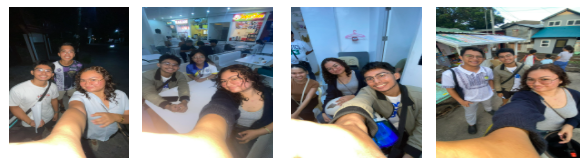
\includegraphics[width=0.90\textwidth,height=0.62\textheight,keepaspectratio]{figures/1.png}
    \caption{Data Flow Diagram}
   \label{fig:dfd_context}
\end{figure}

\hspace*{\parindent}This diagram illustrates how different user groups interact with the KABISIG system. At the top level, the Super Admin (Federation President) manages system configuration, barangay administration, user accounts, federation reports, and audit logs. The Barangay Admin (Chairperson) accesses program details, budget information, documents, announcements, and compliance reports. The SK Officials (Kagawad, Secretary, Treasurer) handle attendance records, budget expenses, documents, feedback, assigned programs, and notifications. Meanwhile, Youth Constituents (residents) receive digital IDs, announcements, program information, and can register, give feedback, and respond to polls. Finally, Viewers (the public) have limited access, viewing announcements, transparency dashboards, and public reports.
\vspace{5mm}

        \begin{figure}[H]
   \centering
         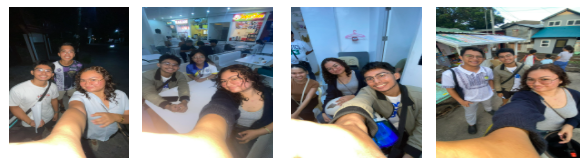
\includegraphics[width=0.90\textwidth,height=0.62\textheight,keepaspectratio]{figures/1.png}
\caption{Data Flow Diagram -- Level 1}
   \label{fig:dfd_level1}
\end{figure}

\hspace*{\parindent}This diagram presents the overall architecture of the KABISIG system, showing how different user roles interact with system modules and databases. The Super Admin oversees system configuration, account management, and audit logs, while the Barangay Admin manages programs, budgets, documents, and compliance reports. The SK Officials handle program schedules, attendance, feedback, and assigned activities. Youth Constituents register, attend programs, provide feedback, and receive digital IDs, while Viewers access public reports and transparency dashboards. The system is organized into six main modules: resident registration and user management, program and attendance management, financial and asset management, document and resolution management, analytics and reporting, and announcement and notification management. Each module connects to specific databases, such as user profiles, program records, attendance logs, feedback, budget, expenses, documents, and announcements.
\vspace{5mm}

\subsubsection{Swimlane Diagram}

\begin{figure}[H]
   \centering
    \includegraphics[width=0.90\textwidth,height=0.62\textheight,keepaspectratio]{figures/swim_lane.png}
    \caption{Swimlane Diagram of KABISIG System}
   \label{fig:swimlane}
\end{figure}

\hspace*{\parindent}The swimlane diagram illustrates the overall workflow of the KABISIG system by showing the responsibilities and interactions of the Youth Constituent, SK Official, KABISIG System, SK Treasurer, and SK Secretary across four major phases: Registration and Account Approval, Program Planning and Registration, Program Execution and Attendance, and Financial Reporting and Records Management. It demonstrates how each actor performs specific tasks, while the system automates processes such as account validation, QR code generation, attendance recording, notifications, report generation, and document management to ensure an organized, transparent, and efficient management of SK programs and services.
\vspace{5mm}

\subsection{Program Flow}

\subsubsection{Resident Registration and Approval}

\begin{figure}[H]
\centering
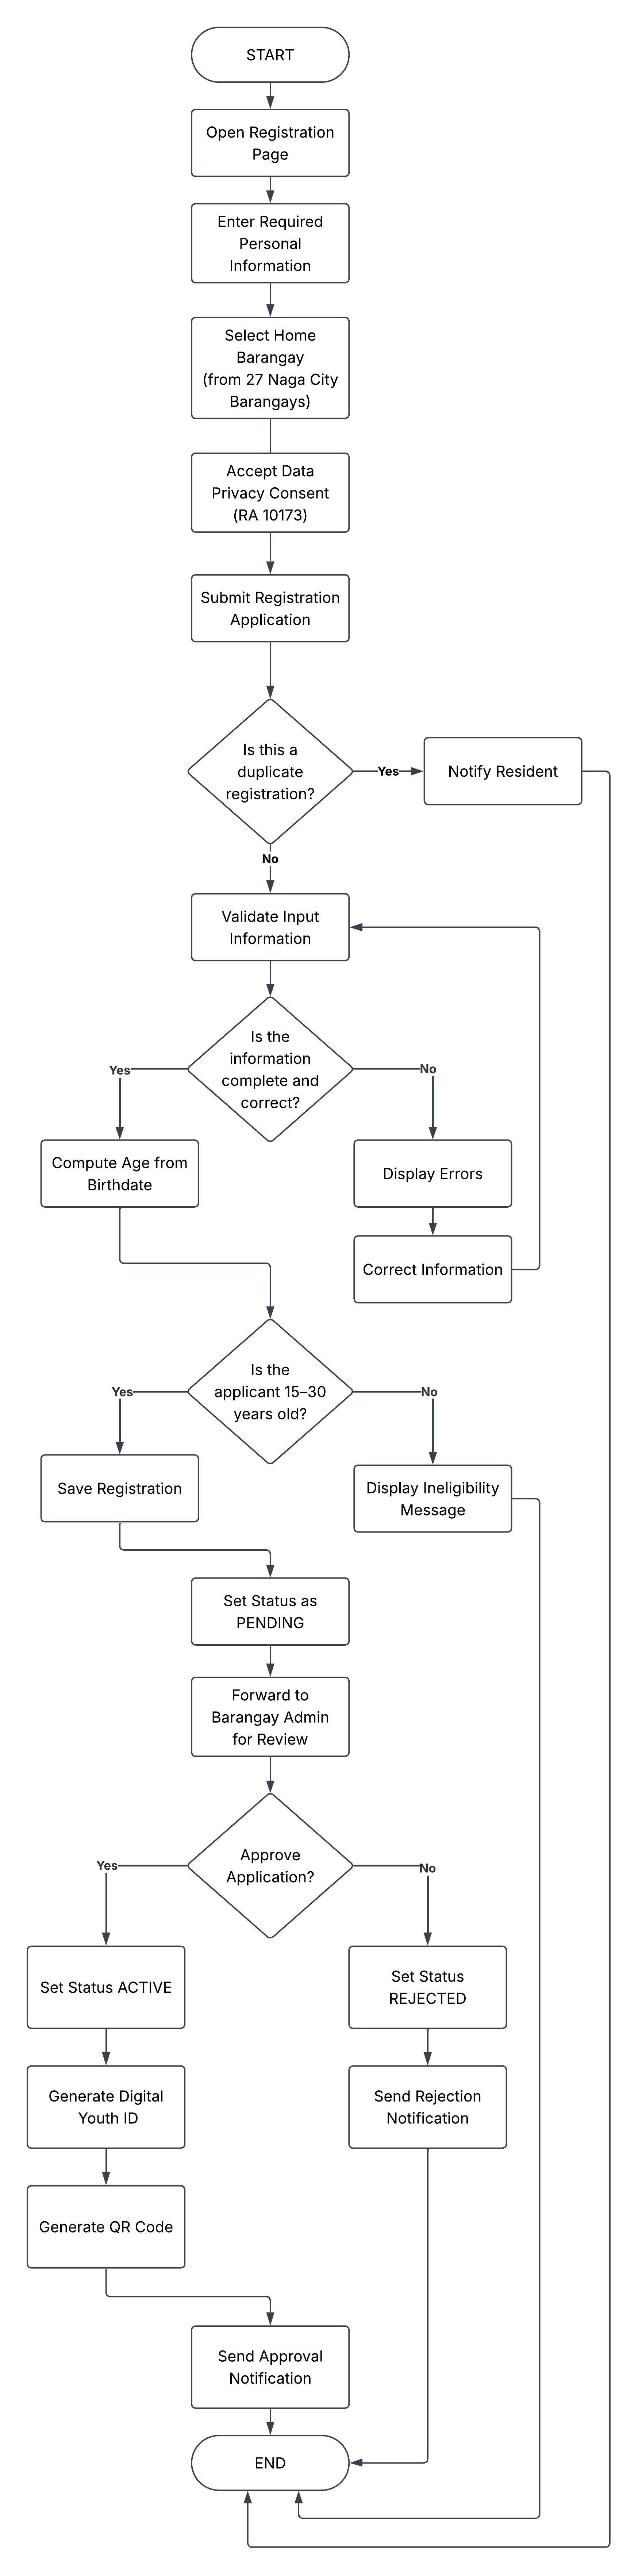
\includegraphics[width=0.90\textwidth,height=0.72\textheight,keepaspectratio]{figures/resident_registraion.png}
\caption{Resident Registration and Approval Activity Diagram}
\label{fig:registration-approval}
\end{figure}

\hspace*{\parindent}This diagram outlines the process of registering a youth constituent for a Digital Youth ID within the KABISIG system. The workflow begins when a youth constituent opens the registration page, enters personal information (full name, birthdate, address, school, guardian details, and other required fields), and submits the application. The system validates the input to check if it is complete and correct, and also validates the youth's age to ensure they are between 15 and 30 years old, as mandated by Republic Act No. 10742. If errors are found, the youth is prompted to correct them before the application proceeds.
\vspace{5mm}

\hspace*{\parindent}Once validated, the registration is saved with a status of pending and is reviewed by the Barangay Administrator or SK Secretary. At this stage, the administrator decides whether to approve or reject the application. Rejected applications trigger a notification to the youth, while approved applications result in the generation of a Digital Youth ID with a QR code for attendance tracking, along with an approval notification sent to the youth.
\vspace{5mm}

\subsubsection{Program Registration and QR Attendance}

\begin{figure}[H]
\centering
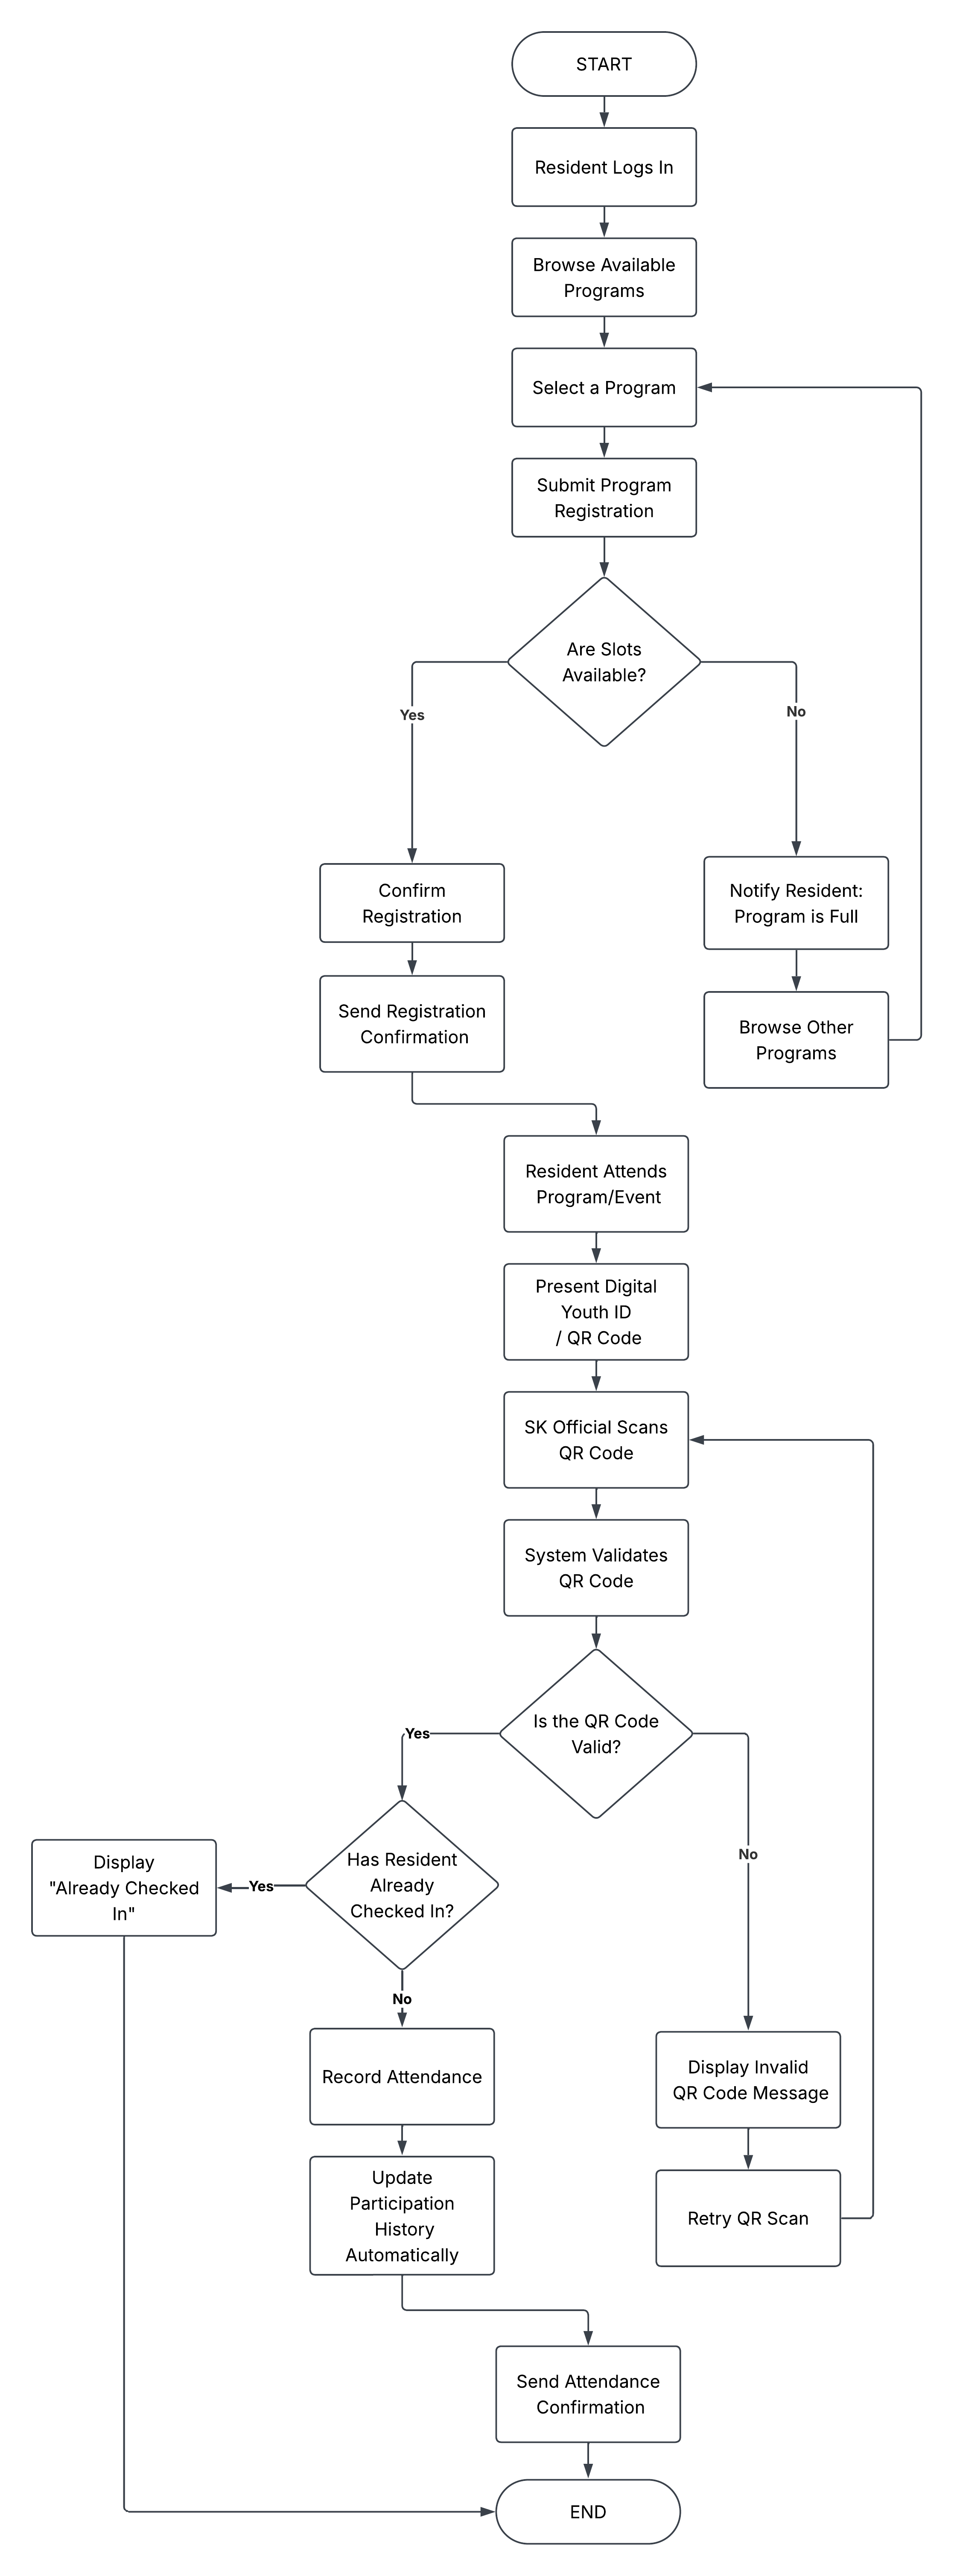
\includegraphics[width=0.90\textwidth,height=0.72\textheight,keepaspectratio]{figures/program_registration.png}
\caption{Program Registration and QR Attendance Activity Diagram}
\label{fig:program-registration}
\end{figure}

\hspace*{\parindent}This diagram shows the process of how residents register and attend programs within the KABISIG system. The workflow begins when a resident logs in, browses available programs, and selects one to join. The system checks slot availability before confirming registration. If slots are full, the resident is notified and directed back to browse other programs. Once registration is confirmed, the resident receives a notification and attends the event. Attendance is validated through QR code scanning, which the system uses to record participation. The resident's participation history is then updated automatically.
\vspace{5mm}

\subsubsection{Budget Management}

\begin{figure}[H]
    \centering
    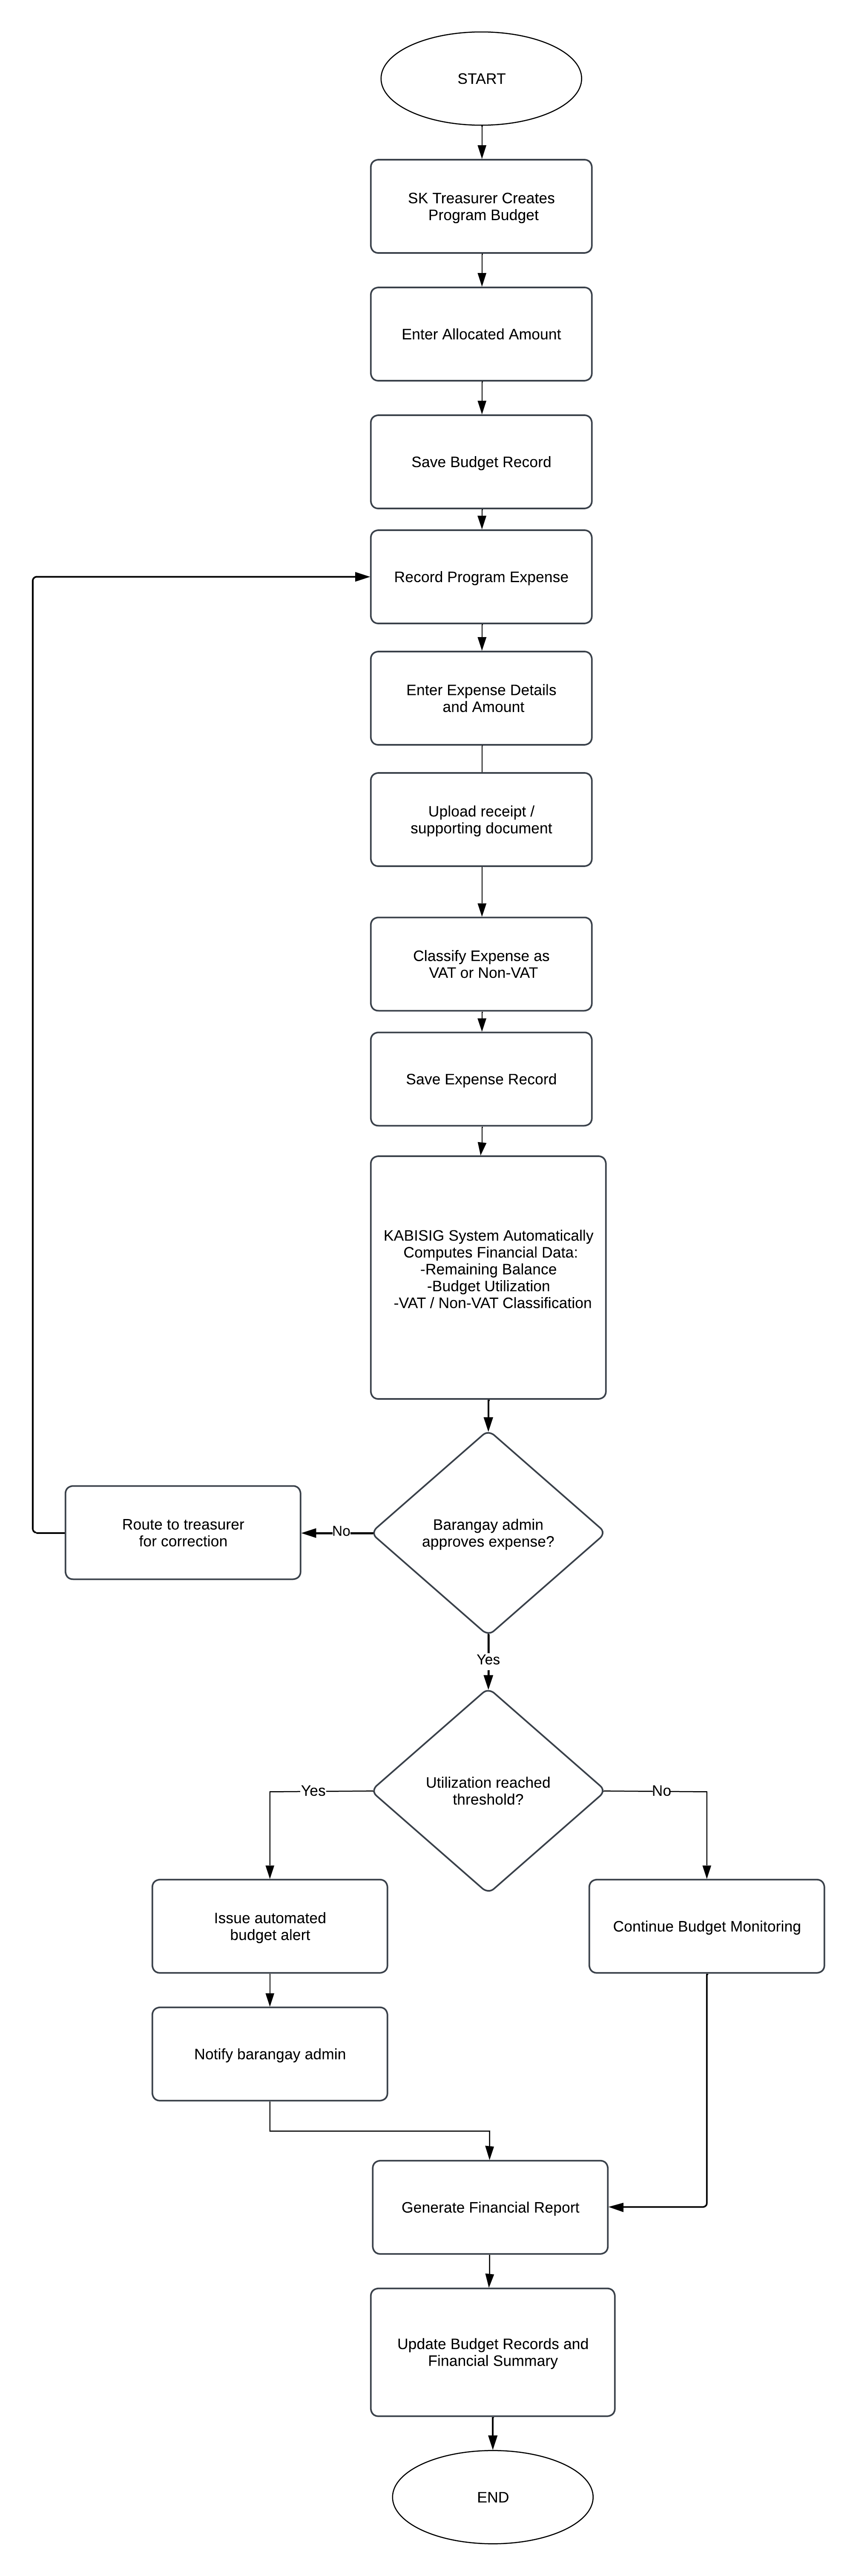
\includegraphics[width=0.90\textwidth,height=0.72\textheight,keepaspectratio]{figures/budget_management.png}
    \caption{Budget Management Activity Diagram}
    \label{fig:budget_management}
\end{figure}

\hspace*{\parindent}This diagram illustrates the process of managing program budgets within the KABISIG system. The workflow begins when the Treasurer creates a budget, enters the allocated amount, and saves the record. Expenses are then recorded, and the system automatically computes the remaining balance, budget utilization, and VAT or non-VAT classification. A decision point checks whether the budget has been exceeded. If not, the process continues normally. If exceeded, the system issues an automated budget alert to notify administrators. In both cases, the workflow leads to the generation of a financial report, which concludes the process.
\vspace{5mm}

\subsubsection{Document Approval Workflow}

\begin{figure}[H]
    \centering
    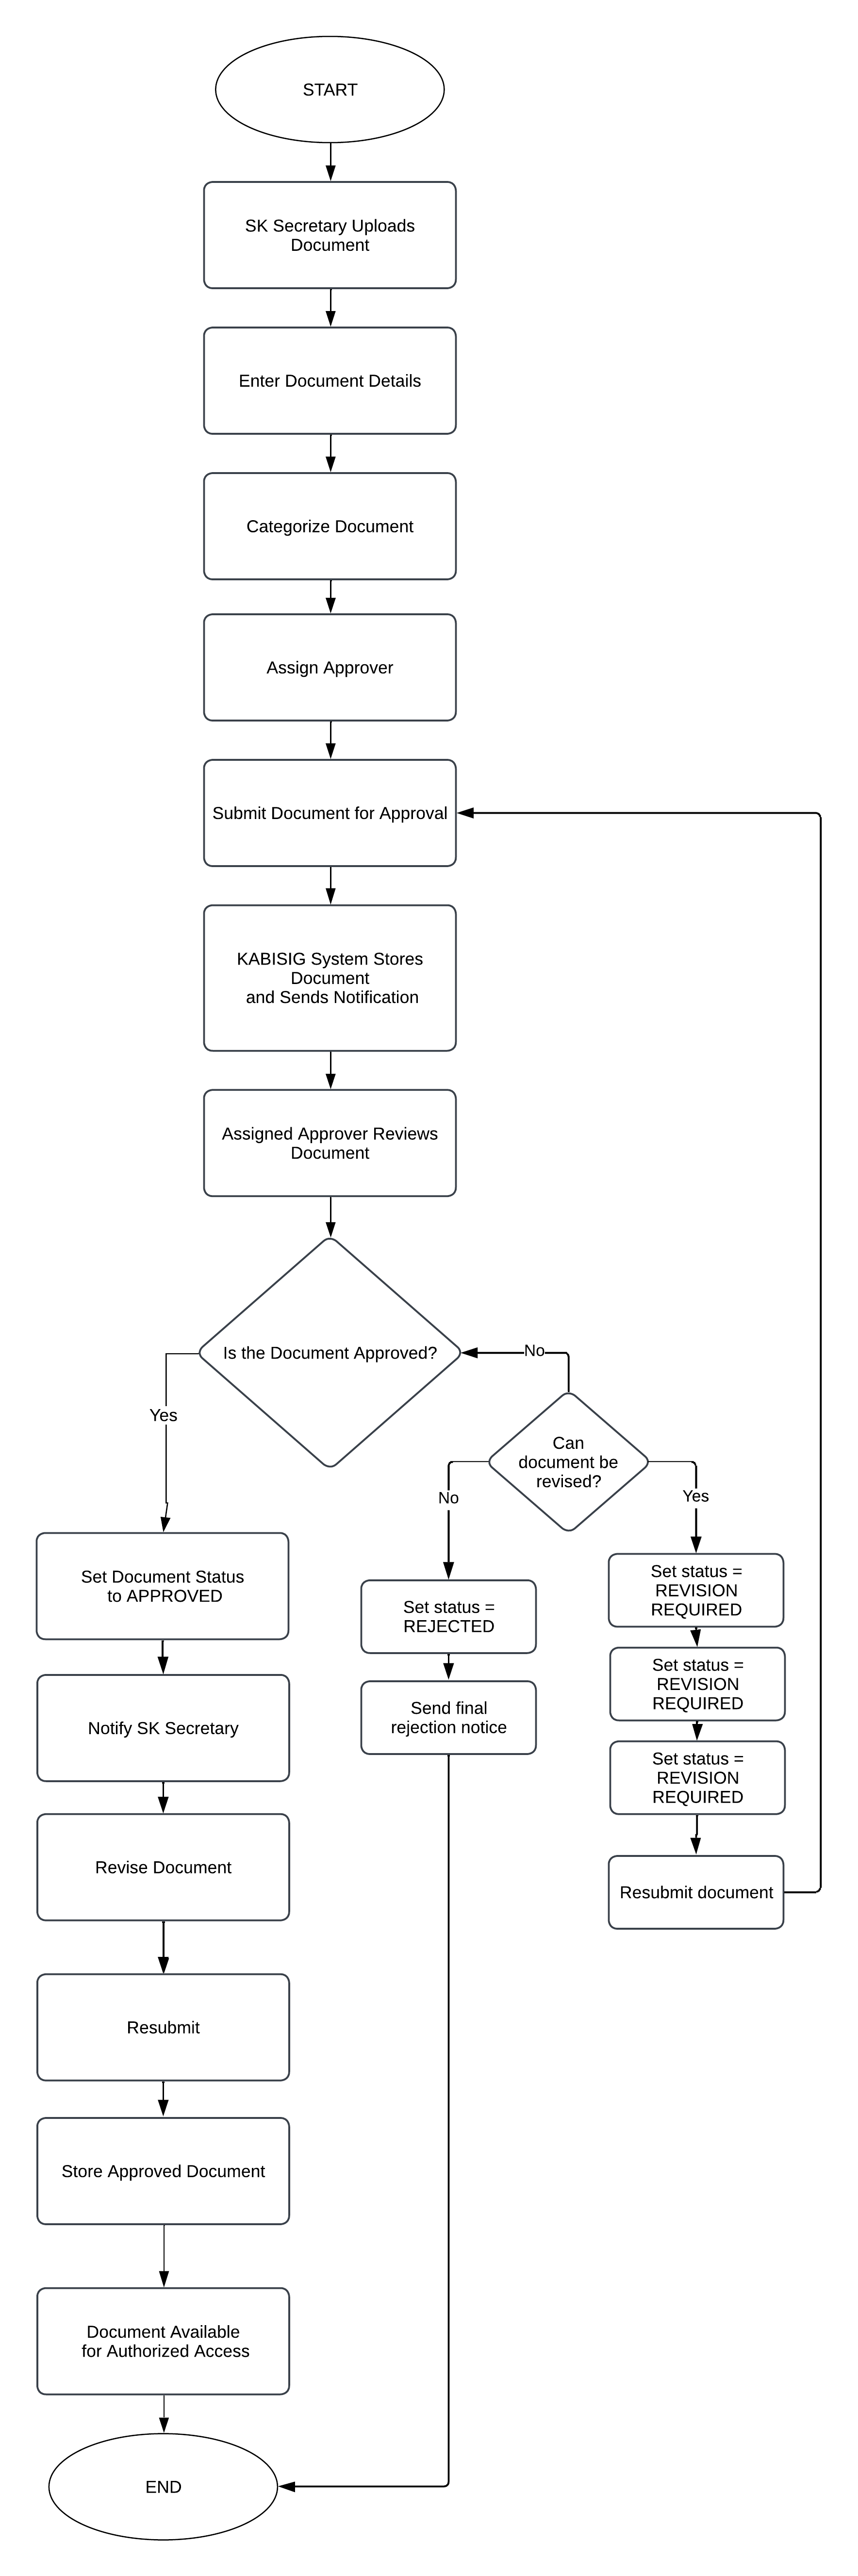
\includegraphics[width=0.90\textwidth,height=0.72\textheight,keepaspectratio]{figures/document_approval.png}
    \caption{Document Approval Workflow}
    \label{fig:document_approval}
\end{figure}

\hspace*{\parindent}This diagram shows the process of document approval within the KABISIG system. The workflow begins when the Secretary uploads a document, categorizes it, and assigns an approver. The approver is notified and reviews the document.
\vspace{5mm}

\subsubsection{Feedback and Automated Analytics}

\begin{figure}[H]
    \centering
    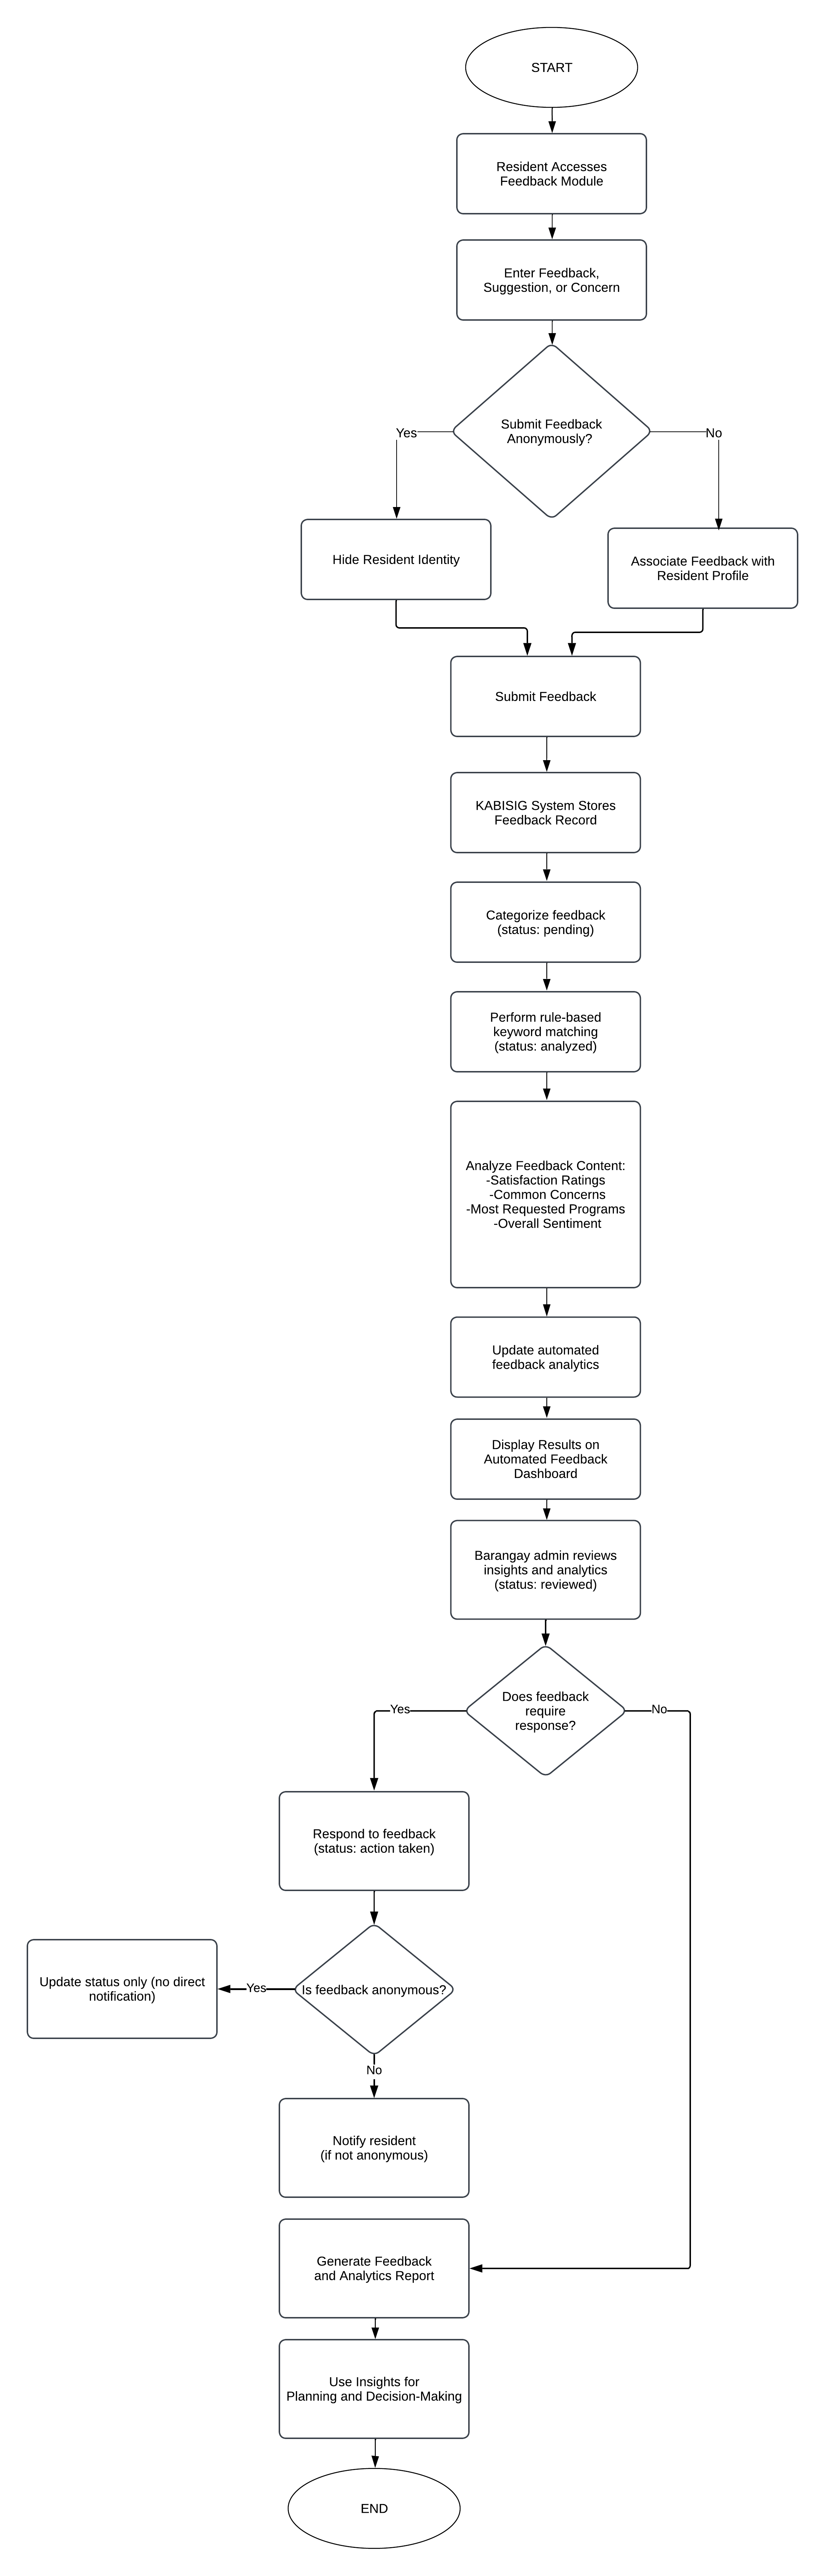
\includegraphics[width=0.90\textwidth,height=0.72\textheight,keepaspectratio]{figures/feedback_automated.png}
    \caption{Feedback and Smart Analytics Activity Diagram}
    \label{fig:feedback_analytics}
\end{figure}

\hspace*{\parindent}This diagram illustrates how resident feedback is collected and processed within the KABISIG system. The process begins when a resident submits feedback, which the system stores and categorizes. The feedback is then analyzed using rule-based keyword matching to update key indicators such as satisfaction ratings, common concerns, most requested programs, and overall sentiment. The results are displayed in an automated feedback dashboard, allowing administrators to review insights and generate reports. The process concludes with the reporting stage, ensuring that feedback is transformed into actionable information.
\vspace{5mm}

\subsubsection{Use Case Diagram}

\begin{figure}[H]
    \centering
    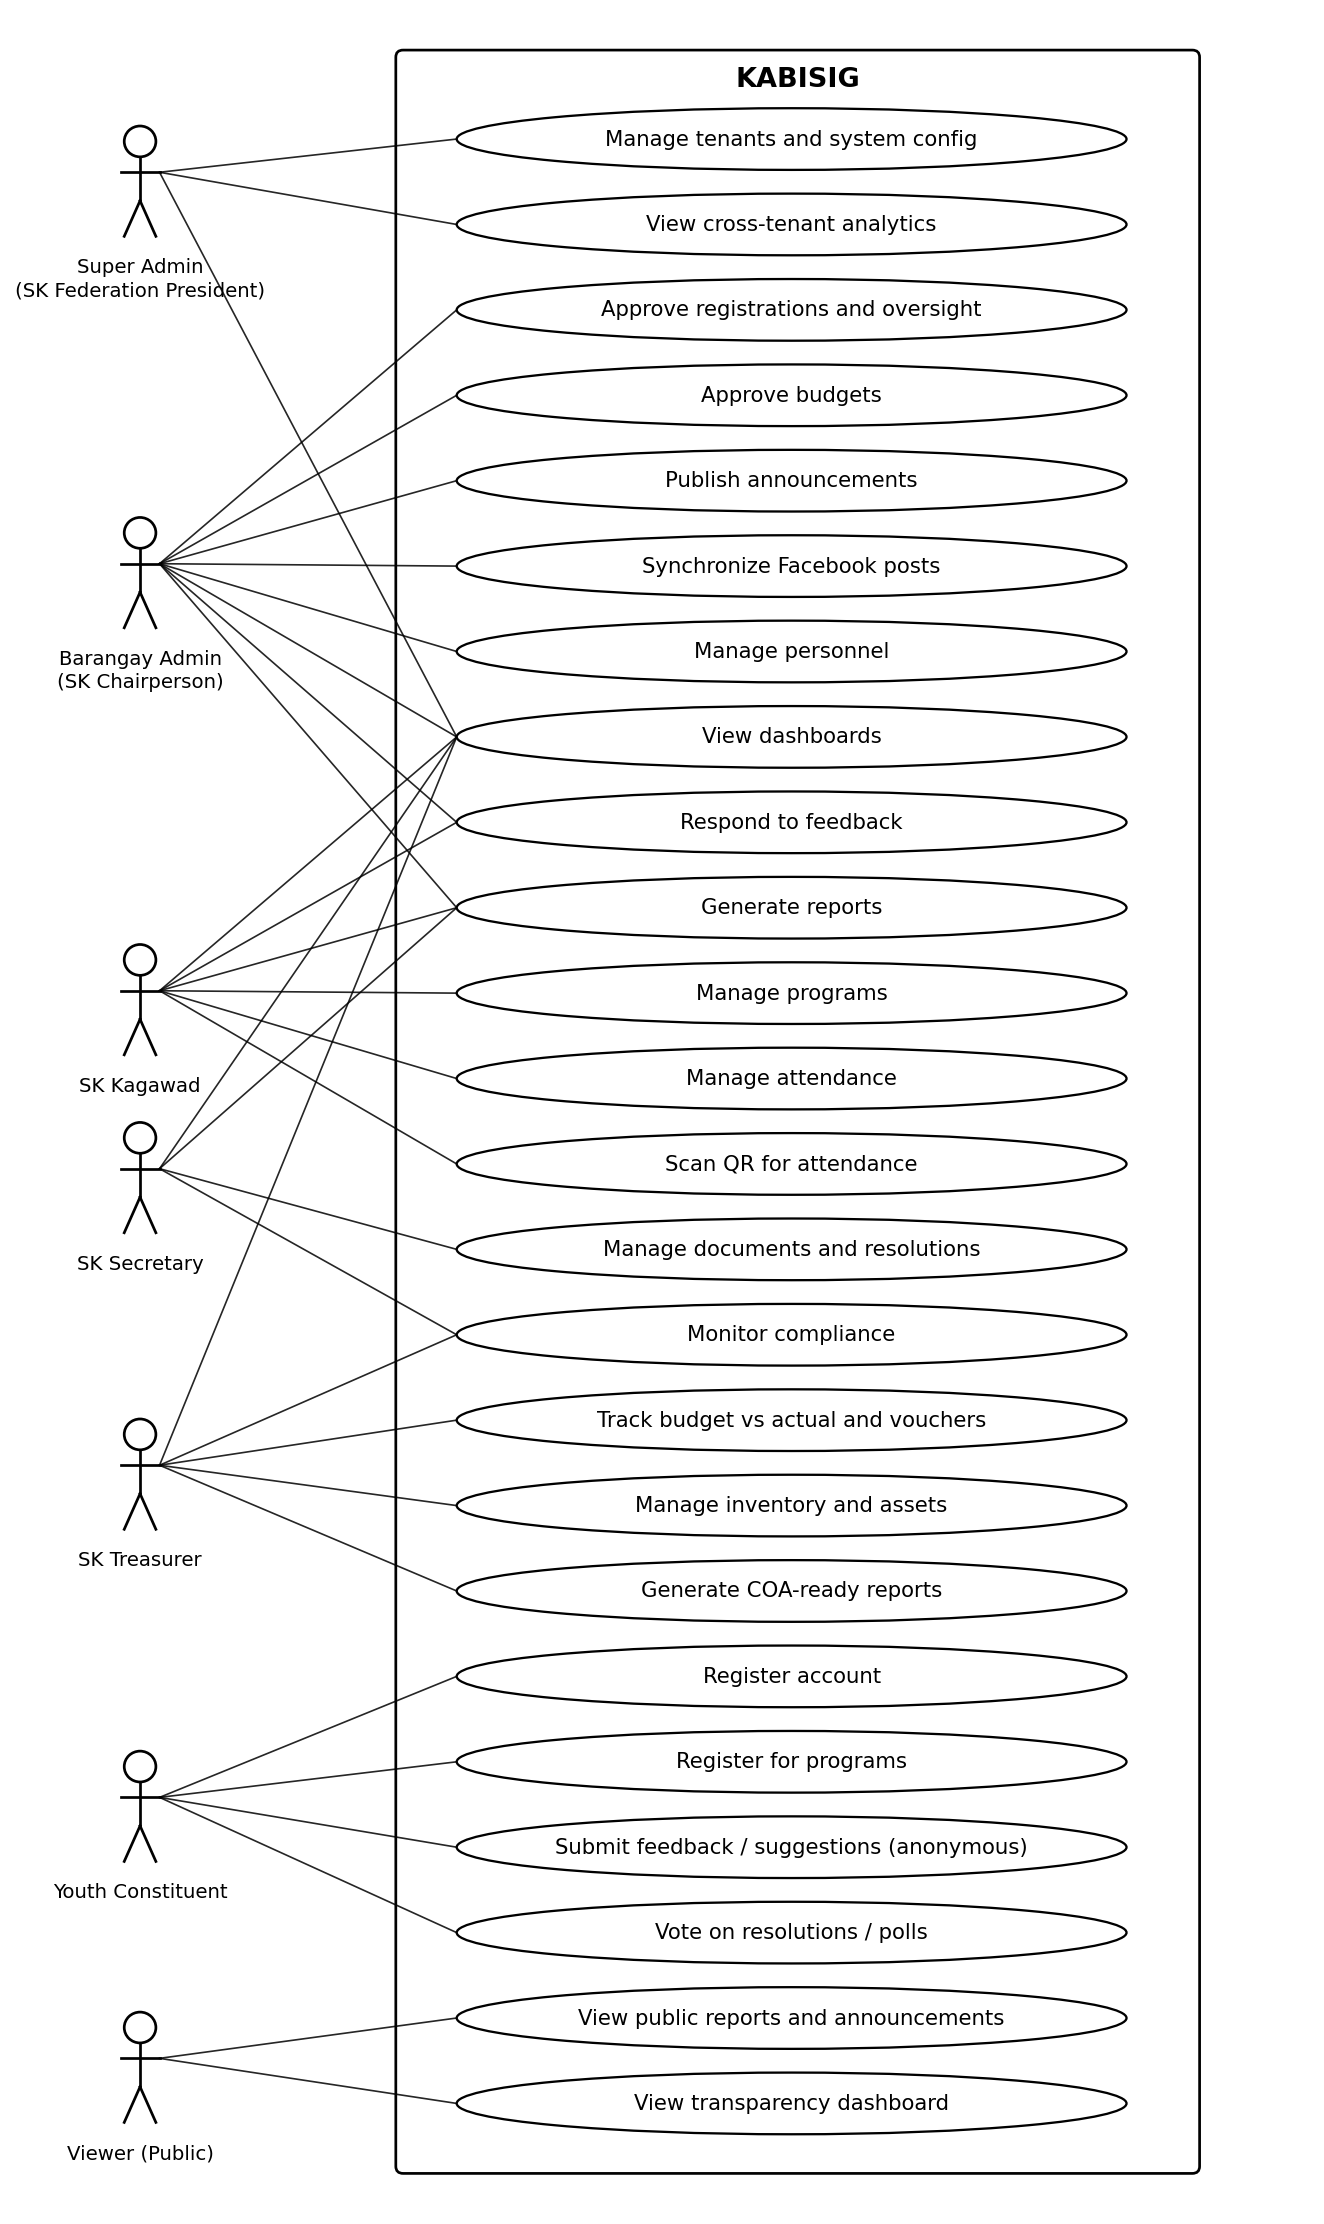
\includegraphics[width=0.90\textwidth,height=0.72\textheight,keepaspectratio]{figures/use_case.png}
    \caption{Use Case Diagram of KABISIG}
    \label{fig:use_case}
\end{figure}


\hspace*{\parindent}This diagram presents the different user roles and their interactions with the KABISIG system. On the administrative side, the Super Admin (Federation President) manages system configuration, personnel, committees, tenants, and cross-barangay analytics. The Barangay Admin (Chairperson) oversees resident profiles, program and event management, budgets, documents, resolutions, and announcements. The SK Officials (Kagawad, Secretary, Treasurer) support program operations, attendance recording, budget and expense management, and document handling. Youth Constituents register accounts, log in, join programs, record attendance via QR codes, submit feedback, and respond to polls. Viewers (public users) have limited access, focusing on announcements and public reports.
\vspace{5mm}

\subsubsection{Entity-Relationship Diagram}

\begin{figure}[H]
    \centering
    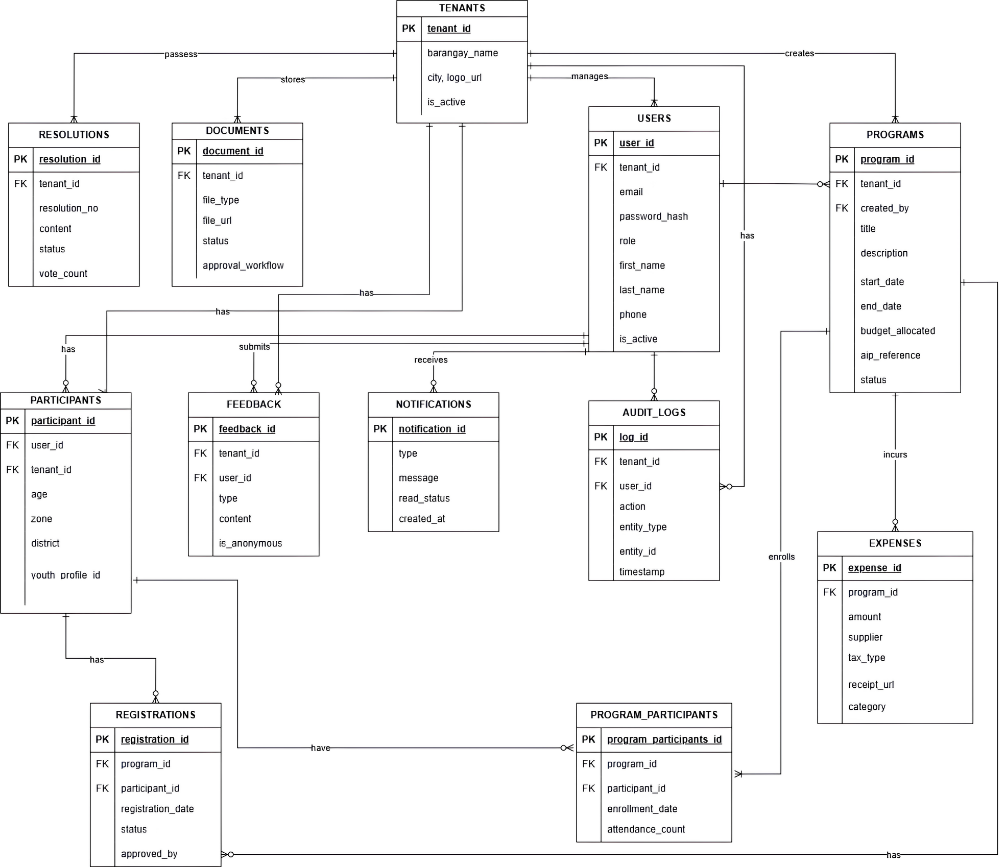
\includegraphics[width=0.90\textwidth,height=0.72\textheight,keepaspectratio]{figures/ERD.png}
    \caption{Entity-Relationship Diagram of KABISIG}
    \label{fig:erd}
\end{figure}

\hspace*{\parindent}The ERD includes the following core and additional entities required for the system's intelligent features:
\vspace{5mm}

\hspace*{\parindent}\textbf{Core Entities:}
\vspace{2mm}

\hspace*{\parindent}ROLES, USERS, BARANGAY, RESIDENT\_PROFILE, PROGRAM, PROGRAM\_REGISTRATIONS, ATTENDANCE, BUDGET, EXPENSE, INVENTORY, DOCUMENT, ANNOUNCEMENT, NOTIFICATIONS, FEEDBACK, POLL, POLL\_RESPONSE, COMMITTEE, COMMITTEE\_ASSIGNMENT, AUDIT\_LOGS
\vspace{5mm}

\hspace*{\parindent}\textbf{Additional Entities:}
\vspace{5mm}

\hspace*{\parindent}\textbf{SENTIMENT\_ANALYSIS}
\begin{itemize}
    \item sentiment\_analysis\_id (UUID, PK)
    \item feedback\_id (UUID, FK to FEEDBACK)
    \item sentiment\_label (VARCHAR 20) -- Positive, Neutral, Negative
    \item sentiment\_score (DECIMAL 3,2)
    \item category (VARCHAR 50)
    \item confidence (DECIMAL 3,2)
    \item response\_status (VARCHAR 20) -- Pending, Analyzed, Reviewed, Action Taken
    \item analyzed\_at (TIMESTAMP)
    \item created\_at (TIMESTAMP)
\end{itemize}
\vspace{5mm}

\hspace*{\parindent}\textbf{COMPLIANCE\_MONITORING}
\begin{itemize}
    \item compliance\_id (UUID, PK)
    \item tenant\_id (UUID, FK to TENANTS)
    \item compliance\_requirement (VARCHAR 255)
    \item compliance\_checklist (JSONB)
    \item report\_deadline (DATE)
    \item compliance\_status (VARCHAR 50) -- Pending, In Progress, Completed, Overdue
    \item submitted\_at (TIMESTAMP)
    \item submitted\_by (UUID, FK to USERS)
    \item approved\_by (UUID, FK to USERS)
    \item approved\_at (TIMESTAMP)
    \item reminder\_sent (BOOLEAN)
    \item created\_at (TIMESTAMP)
\end{itemize}
\vspace{5mm}

\hspace*{\parindent}\textbf{SOCIAL\_MEDIA\_POSTS}
\begin{itemize}
    \item social\_post\_id (UUID, PK)
    \item announcement\_id (UUID, FK to ANNOUNCEMENTS)
    \item tenant\_id (UUID, FK to TENANTS)
    \item facebook\_post\_id (VARCHAR 100)
    \item post\_content (TEXT)
    \item post\_status (VARCHAR 20) -- Draft, Scheduled, Posted, Failed
    \item scheduled\_time (TIMESTAMP)
    \item published\_time (TIMESTAMP)
    \item sync\_status (VARCHAR 20) -- Pending, Synced, Error
    \item error\_message (TEXT)
    \item created\_by (UUID, FK to USERS)
    \item created\_at (TIMESTAMP)
    \item updated\_at (TIMESTAMP)
\end{itemize}
\vspace{5mm}

\subsection{Development and Testing}

\subsubsection{Requirements Gathering}

\hspace*{\parindent}Requirements were collated through:
\vspace{5mm}

\begin{enumerate}
    \item Interviews with SK members such as the SK Chairperson, Kagawad, Secretary, and Treasurer to uncover issues and requirements in Naga City barangays.
    \item Review of previous reports, attendance sheets, word-processed plans, and governance documents.
    \item Analysis of existing resources including spreadsheets for tracking participants, Facebook/Messenger announcements, and manual filing systems for documents.
    \item Observation of manual processes during SK programs, SK meetings, and barangay council meetings.
    \item Review and gap analysis of panel recommendations for the current SK information systems.
\end{enumerate}
\vspace{5mm}

\subsection{Account Creation and Approval Workflow}

\hspace*{\parindent}Based on the requirements gathering activities, the following account creation and approval workflow was established:
\vspace{5mm}

\hspace*{\parindent}\textbf{Super Administrator:} The account is pre-created by the system developer during initial deployment and does not require approval from anyone, as no authority above the Super Administrator exists within the system. The SK Federation President receives credentials through a secure offline handoff and is required to change their password on first login.
\vspace{5mm}

\hspace*{\parindent}\textbf{Barangay Administrator (SK Chairperson):} The account is created directly by the Super Administrator through the Barangay Management module. The SK Chairperson does not self-register; instead, the Super Admin enters their details and the account is created with status = active immediately. The act of creation serves as the approval, reflecting the real-world process where SK Chairpersons are appointed by the SK Federation President.
\vspace{5mm}

\hspace*{\parindent}\textbf{SK Officials (Kagawad, Secretary, Treasurer):} Officials self-register through the public portal but cannot access the system until their account is approved by the Barangay Administrator. Upon registration, accounts are created with status = pending. The Barangay Admin receives a notification, reviews the applicant's details, and approves or rejects the registration through the User Management $\rightarrow$ Pending Accounts module. If approved, status changes to active and approved\_by is set to the Barangay Admin's user\_id.
\vspace{5mm}

\hspace*{\parindent}\textbf{Youth Constituents:} Youth self-register through the public youth portal, with accounts created in a pending state. The system validates age (15-30 years old) during registration. Barangay Administrators or assigned SK Officials review and approve youth registrations through the Youth Management $\rightarrow$ Pending Registrations module. Upon approval, the system automatically generates a Digital Youth ID with a QR code for attendance tracking.
\vspace{5mm}

\hspace*{\parindent}\textbf{Viewers:} Viewers do not require accounts. They access public-facing pages (Transparency Dashboard, Announcements, Program Schedules) without authentication. All public data is anonymized and aggregated for privacy compliance.
\vspace{5mm}

\hspace*{\parindent}This hierarchical approval workflow ensures that only verified barangay administrators manage SK operations, SK officials are legitimate council members appointed by their chairperson, youth constituents are verified residents within the 15-30 age range, and public transparency is maintained without creating barriers to access.
\vspace{5mm}

\section{Functional Requirements}

\subsection{System Features}

\hspace*{\parindent}The KABISIG system integrates multiple modules to support youth governance, program management, financial transparency, and community engagement. Each module provides specific functionalities that collectively ensure accountability, efficiency, and inclusivity.
\vspace{5mm}

\textbf{1. Resident Profiling and Participant Management}
\begin{itemize}
    \item \textbf{Resident Profiling} -- Keeps detailed records of residents' personal and community information.
    \item \textbf{Participant Registration, Verification, and Approval} -- Allows online sign-up with admin approval before access.
    \item \textbf{Demographic Categorization} -- Groups residents by status (e.g., student, scholar, employed, unemployed).
    \item \textbf{Zone- and District-Based Tracking} -- Organizes residents by geographic areas for easier monitoring.
    \item \textbf{Digital Resident ID Generation} -- Issues a unique digital ID for each approved participant.
    \item \textbf{QR Code Attendance Management} -- Records attendance using QR codes and prevents duplicate check-ins.
    \item \textbf{Beneficiary and Participation Monitoring} -- Tracks assistance received and participation history.
    \item \textbf{Automated Engagement Analytics} -- Calculates engagement scores using rule-based logic.
\end{itemize}
\vspace{5mm}

\textbf{2. Program, Event, and Community Governance Management}
\begin{itemize}
    \item \textbf{Program and Event Management} -- Enables creation, scheduling, and evaluation of activities.
    \item \textbf{Integrated Calendar Management} -- Centralizes schedules to avoid overlaps and conflicts.
    \item \textbf{Development Plan Monitoring} -- Monitors implementation of approved development plans.
    \item \textbf{Resolution and Ordinance Management} -- Handles drafting, approval, and archiving of official SK documents.
    \item \textbf{Committee and Responsibility Assignment} -- Assigns roles and responsibilities for projects and events.
    \item \textbf{Community Polling and Surveys} -- Collects opinions and votes from residents for decision-making.
    \item \textbf{Program Participation Monitoring} -- Tracks registrations, attendance, and completion of programs.
    \item \textbf{Automated Schedule Conflict Detection} -- Detects overlapping programs and schedule inconsistencies.
\end{itemize}
\vspace{5mm}

\textbf{3. Financial Transparency and Resource Management}
\begin{itemize}
    \item \textbf{Budget Allocation and Utilization Monitoring} -- Tracks how funds are assigned and spent for programs.
    \item \textbf{Automated Financial Computations} -- Calculates balances, utilization rates, and taxes automatically (VAT/Non-VAT).
    \item \textbf{Expense, Liquidation, and Receipt Management} -- Records and organizes financial transactions.
    \item \textbf{Budget Reversion Monitoring} -- Tracks unused funds available for reallocation or reversion.
    \item \textbf{Automated Budget Monitoring} -- Analyzes spending, detects overspending, and sends alerts.
    \item \textbf{Inventory and Asset Management} -- Keeps records of equipment, supplies, and other assets.
    \item \textbf{Asset Turnover Tracking} -- Monitors issuance, return, transfer, and disposal of assets.
    \item \textbf{Public Transparency Dashboard} -- Shows summarized financial data for public viewing.
\end{itemize}
\vspace{5mm}

\textbf{4. Document and Records Management}
\begin{itemize}
    \item \textbf{Centralized Document Repository} -- Stores all official documents securely in one place.
    \item \textbf{Document Categorization and Status Tracking} -- Organizes documents by type and monitors their progress.
    \item \textbf{Digital Approval Workflow} -- Routes documents electronically to designated signatories.
    \item \textbf{Automated PDF Report Generation} -- Creates reports like attendance sheets and financial summaries.
    \item \textbf{Automated Compliance Monitoring} -- Tracks pending approvals, overdue reports, and missing documents.
\end{itemize}
\vspace{5mm}

\textbf{5. Community Engagement and Feedback Management}
\begin{itemize}
    \item \textbf{Community Feedback Platform} -- Provides a platform for residents to share concerns and suggestions.
    \item \textbf{Suggestions and Concern Submission} -- Allows residents to submit requests and complaints.
    \item \textbf{Anonymous Feedback Support} -- Enables anonymous reporting to encourage honest participation.
    \item \textbf{Program and Project Evaluation} -- Collects participant ratings and feedback after activities.
    \item \textbf{Community Consultations and Surveys} -- Conducts surveys to support evidence-based planning.
    \item \textbf{Automated Feedback Analysis} -- Uses keyword-based (rule-based) classification to summarize feedback into concerns, requested programs, and sentiment.
\end{itemize}
\vspace{5mm}

\textbf{6. Analytics, Reporting, and Decision Support}
\begin{itemize}
    \item \textbf{Real-time Dashboards} -- Shows live summaries of registrations, attendance, budgets, and programs.
    \item \textbf{Program Performance Analytics} -- Measures participation, completion rates, satisfaction, and budget use.
    \item \textbf{Demographic and Beneficiary Analytics} -- Analyzes resident demographics and distribution of beneficiaries.
    \item \textbf{Attendance and Engagement Analytics} -- Identifies trends in participation and engagement levels.
    \item \textbf{Cross-Community Analytics} -- Compares performance and statistics across different barangays.
\end{itemize}
\vspace{5mm}

\textbf{7. Notification and Communication Management}
\begin{itemize}
    \item \textbf{Announcements and Broadcasts} -- Publishes official announcements and advisories.
    \item \textbf{Program and Event Reminders} -- Sends reminders before, during, and after activities.
    \item \textbf{Registration and Approval Notifications} -- Notifies users about registration status and approvals.
    \item \textbf{Calendar-Based Alerts} -- Generates alerts based on scheduled events and deadlines.
    \item \textbf{Compliance Reminders} -- Reminds personnel about upcoming reports, approvals, and compliance tasks.
\end{itemize}
\vspace{5mm}

\textbf{8. Organization and Personnel Management}
\begin{itemize}
    \item \textbf{Organizational Structure Management} -- Maintains the SK organizational chart and hierarchy.
    \item \textbf{Personnel Profiles and Role Management} -- Manages user accounts, roles, and access permissions.
    \item \textbf{Committee and Responsibility Management} -- Assigns committees and tracks responsibilities.
    \item \textbf{Personnel Attendance Monitoring} -- Records attendance during meetings and official activities.
    \item \textbf{Performance and Compliance Monitoring} -- Tracks personnel participation and compliance with tasks.
    \item \textbf{Administrative Oversight Dashboard} -- Provides administrators with organization-wide monitoring tools.
\end{itemize}
\vspace{5mm}

\textbf{9. Social Media Integration and Public Information}
\begin{itemize}
    \item \textbf{Official Facebook Page Integration} -- Connects the system to the SK's official Facebook page.
    \item \textbf{Automatic Announcement Synchronization} -- Publishes approved announcements directly to Facebook.
    \item \textbf{Scheduled Facebook Posting} -- Allows announcements to be posted automatically at set times.
    \item \textbf{Auto-generated Facebook Posts} -- Formats posts with event details, images, and QR codes.
    \item \textbf{Public Information Synchronization} -- Ensures consistency of public announcements between KABISIG and Facebook.
    \item \textbf{Post Status Tracking} -- Monitors posts with status: Draft, Scheduled, Posted, Failed.
\end{itemize}
\vspace{5mm}

\subsubsection{Sprint Planning}

\begin{table}[H]
\centering
\caption{Sprint Planning Phases}
\label{tab:sprint-planning}
\small
\begin{tabular}{|p{2.5cm}|p{1.5cm}|p{4cm}|p{5.5cm}|}
\hline
\textbf{Phase} & \textbf{Duration} & \textbf{Focus} & \textbf{Key Deliverables} \\
\hline
Phase 1: Planning and Documentation & Months 1--2 & Planning the project, identifying the system requirements, performing the analysis and designing of the system. & Completion of system requirements, scope and limitations, definition of user roles, use case scenarios, database design, UI/UX prototyping, system architecture design, project documentation and development plan. \\
\hline
Phase 2: Foundation Development & Month 3 & Designing the architecture and functionalities of the system. & Authentication processes, role based authorization, multi-tenancy, user management, database development, initial system interface, and web responsive design. \\
\hline
Phase 3: Core Operations Development & Month 4 & SK management functionality implementation. & Youth profiling, participant registration, program management, calendar management, attendance management, expense tracking, budgeting and simple report generation. \\
\hline
Phase 4: Governance and Engagement Features & Month 5 & Designing the modules to provide transparency and youth engagement. & Feedback management system for Boses ng Kabataan, issue management, youth survey, document and record management, notifications and public viewing capabilities. \\
\hline
Phase 5: Analytics and System Integration & Month 6 & Adding advanced functionalities and enhancements of the system. & Dashboards analytics, federation level analytics, automated reports, mobile responsiveness and API services. \\
\hline
Phase 6: Testing, Deployment, and Optimization & Month 7 & System testing, refinement, and preparation for deployment. & Functional testing, usability testing, User Acceptance Testing (UAT), security testing, performance tuning, bug fixing, user feedback driven improvements, user documentation and training material development. \\
\hline
\end{tabular}
\end{table}
\vspace{5mm}

\subsection{Version Control}

\hspace*{\parindent}The process utilizes Git version control which allows tracking changes made to the code, collaboration between developers, and reverting to a reliable version whenever necessary. Branch protection policies, pull request reviews, and continuous integration pipelines via GitHub Actions in total provide for the high-quality and stable nature of the code.
\vspace{5mm}

\subsection{Testing and Evaluation Procedures}

\subsubsection{Types of Testing}

\hspace*{\parindent}\textbf{Functional Testing:} Evaluation will cover CRUD operations, internal reports, RBAC, multi-tenancy, document approval process, notification functionality, and the precision of budget computations. Such approach is typical for software testing according to ISO 25010 and will be used to evaluate similar barangay information systems.
\vspace{5mm}

\hspace*{\parindent}\textbf{Usability Testing:} The usability evaluation will focus on the ease of navigation for the SK representatives and youth users in both the web and mobile versions of the system in terms of success rate of performing such tasks as creating programs, registration, giving feedback, and uploading documents. In order to assess the user satisfaction level, Technology Acceptance Model (TAM) and the Unified Theory of Acceptance and Use of Technology (UTAUT) will be used.
\vspace{5mm}

\hspace*{\parindent}\textbf{Performance Testing:} Evaluation will include real-time data processing, load time less than 2 seconds, API response time less than 500 ms, PDF creation time, and notification dispatch latency.
\vspace{5mm}

\hspace*{\parindent}\textbf{Security Testing:} Evaluation will include server-side security, RBAC, enforcement of RLS policies, data encryption, protection against penetration, and document access management. This corresponds to ISO/IEC 27001:2022 requirements.
\vspace{5mm}

\hspace*{\parindent}\textbf{Cross-Browser and Mobile Compatibility Testing:} Evaluation will include functional tests, layout consistency, and responsiveness in such popular browsers as Chrome, Firefox, Edge, Safari for desktop users and iOS Safari, Android Chrome for mobile users without the need for developing a dedicated app.
\vspace{5mm}

\subsubsection{Evaluation Criteria and Metrics}

\hspace*{\parindent}The system was evaluated using a five-point Likert scale based on:
\vspace{5mm}

\hspace*{\parindent}\textbf{ISO 25010 Software Quality Model:}
\begin{itemize}
    \item Functional Suitability
    \item Usability
    \item Performance Efficiency
    \item Reliability
    \item Security
\end{itemize}
\vspace{5mm}

\hspace*{\parindent}\textbf{Technology Acceptance Model (TAM):}
\begin{itemize}
    \item Perceived Usefulness (PU)
    \item Perceived Ease of Use (PEOU)
    \item Behavioral Intention to Use
    \item Actual System Use
\end{itemize}
\vspace{5mm}

\hspace*{\parindent}\textbf{Unified Theory of Acceptance and Use of Technology (UTAUT):}
\begin{itemize}
    \item Performance Expectancy
    \item Effort Expectancy
    \item Social Influence
    \item Facilitating Conditions
\end{itemize}
\vspace{5mm}

\hspace*{\parindent}\textbf{Custom Engagement Metrics:}
\begin{itemize}
    \item Monthly Active Users (MAU): Target $\geq$ 60\%
    \item Program Registration Rate: Target $\geq$ 90\%
    \item Attendance Rate: Target $\geq$ 75\%
    \item Feedback Submission Rate: Target $\geq$ 40\%
    \item SK Official Adoption Rate: Target $\geq$ 80\%
    \item Document Processing Time: Target $\leq$ 50\% reduction vs. manual
    \item Budget Reporting Accuracy: Target $\geq$ 98\%
\end{itemize}
\vspace{5mm}

\subsection{Implementation and Deployment Plan}

\subsubsection{Deployment Environment}

\hspace*{\parindent}Vercel is a tool used to deploy websites with automatic optimization of performance, serverless hosting, and secured handling of environment variables. The system is mobile responsive, allowing use of all features on any mobile web browser available without having to install another application. Supabase manages hosting of PostgreSQL with automatic backups, point in time recovery, row level security, real time databases, and geographical redundancy.
\vspace{5mm}

\subsubsection{User Training and Documentation}

\hspace*{\parindent}Users were oriented through:
\vspace{5mm}

\begin{enumerate}
    \item Organized system demonstrations for SK officials across Naga City barangays
    \item Step-by-step system usage guides for each user role
    \item Video tutorials for youth self-registration, feedback submission, and document upload
    \item Administrator documentation for tenant management, RBAC configuration, and document approval workflow setup
    \item SK Secretary/Treasurer-specific guides for document management and financial reporting
    \item Super Administrator training for cross-barangay analytics interpretation
\end{enumerate}
\vspace{5mm}

\subsubsection{Maintenance and Future Enhancements}

\hspace*{\parindent}The system is adaptable for future modifications:
\vspace{5mm}

\begin{itemize}
    \item Sophisticated analysis and advanced reporting on budget and program outcomes
    \item Email and SMS notification dissemination
    \item Enhanced mobile-responsive interface features
    \item Reinforced data protection, backup, and recovery protocols
    \item Interoperability APIs for national government database integration
    \item Integration with Naga City government digital services
\end{itemize}
\vspace{5mm}

\subsection{Summary}

\hspace*{\parindent}The methodology ensures that the project, KABISIG, uses an agile approach in accordance with internationally approved evaluation standards. The system thus increases its usefulness in solving operational challenges of the Sangguniang Kabataan program and participants in an effective manner. The step-by-step approach allows systematic validation at each phase while incorporating feedback from SK officials, and youth participants.
\vspace{5mm}

\subsection{User Interface and System Screens}

\hspace*{\parindent}The KABISIG system features a clean, modern, and mobile-responsive user interface designed to provide an intuitive experience across all user roles. The interface follows a consistent design language with the KABISIG color palette (Deep Blue \#1a237e, Vibrant Red \#d32f2f, White \#ffffff, and Gold \#fdd835) and a minimalist, government-appropriate aesthetic. Each screen is designed with the user's role and tasks in mind, ensuring efficient navigation and task completion.
\vspace{5mm}

\hspace*{\parindent}\textbf{Note:} The data presented in all screenshots are sample/placeholder data used for demonstration purposes only. They do not represent actual SK records, financial transactions, or personal information of any barangay, official, or youth constituent.
\vspace{5mm}

\subsubsection{Public Screens and Authentication}

\hspace*{\parindent}The public-facing screens provide unauthenticated users with access to system information and registration capabilities. The Public Transparency Portal allows citizens to view SK financial data, budget utilization, and program expenditures. This screen displays key metrics including city youth demographics, total federation budget, and total disbursed funds with utilization percentage. The Municipal Public Auditing Desk provides detailed expense tracking with transaction details, supplier information, and tax classifications.
\vspace{5mm}

\begin{figure}[H]
\centering
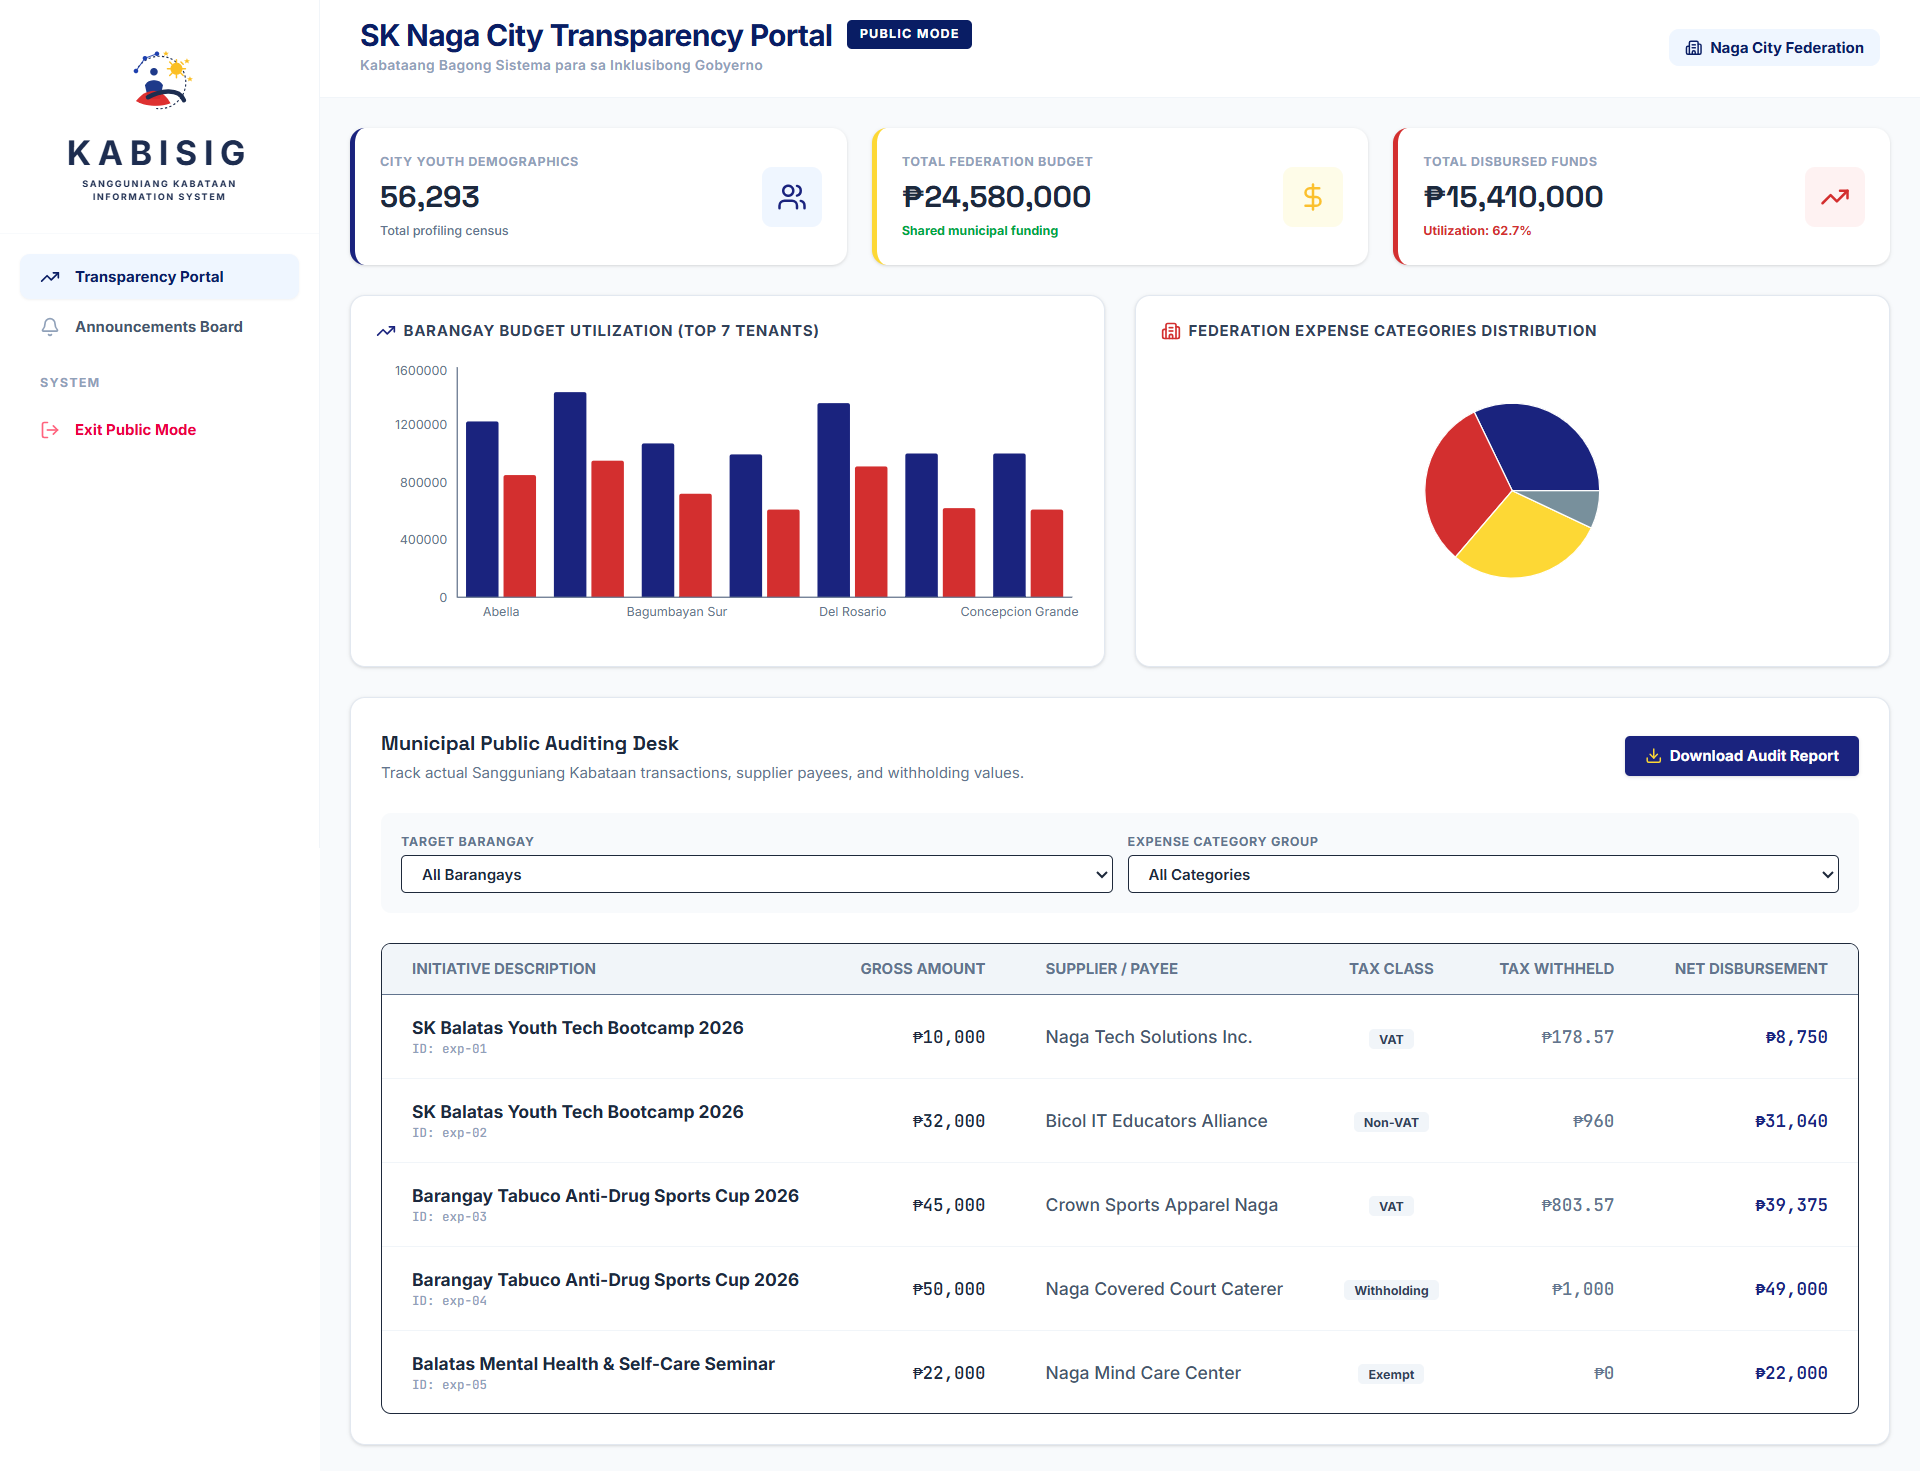
\includegraphics[width=0.45\textwidth]{figures/transparency_portal1.png}
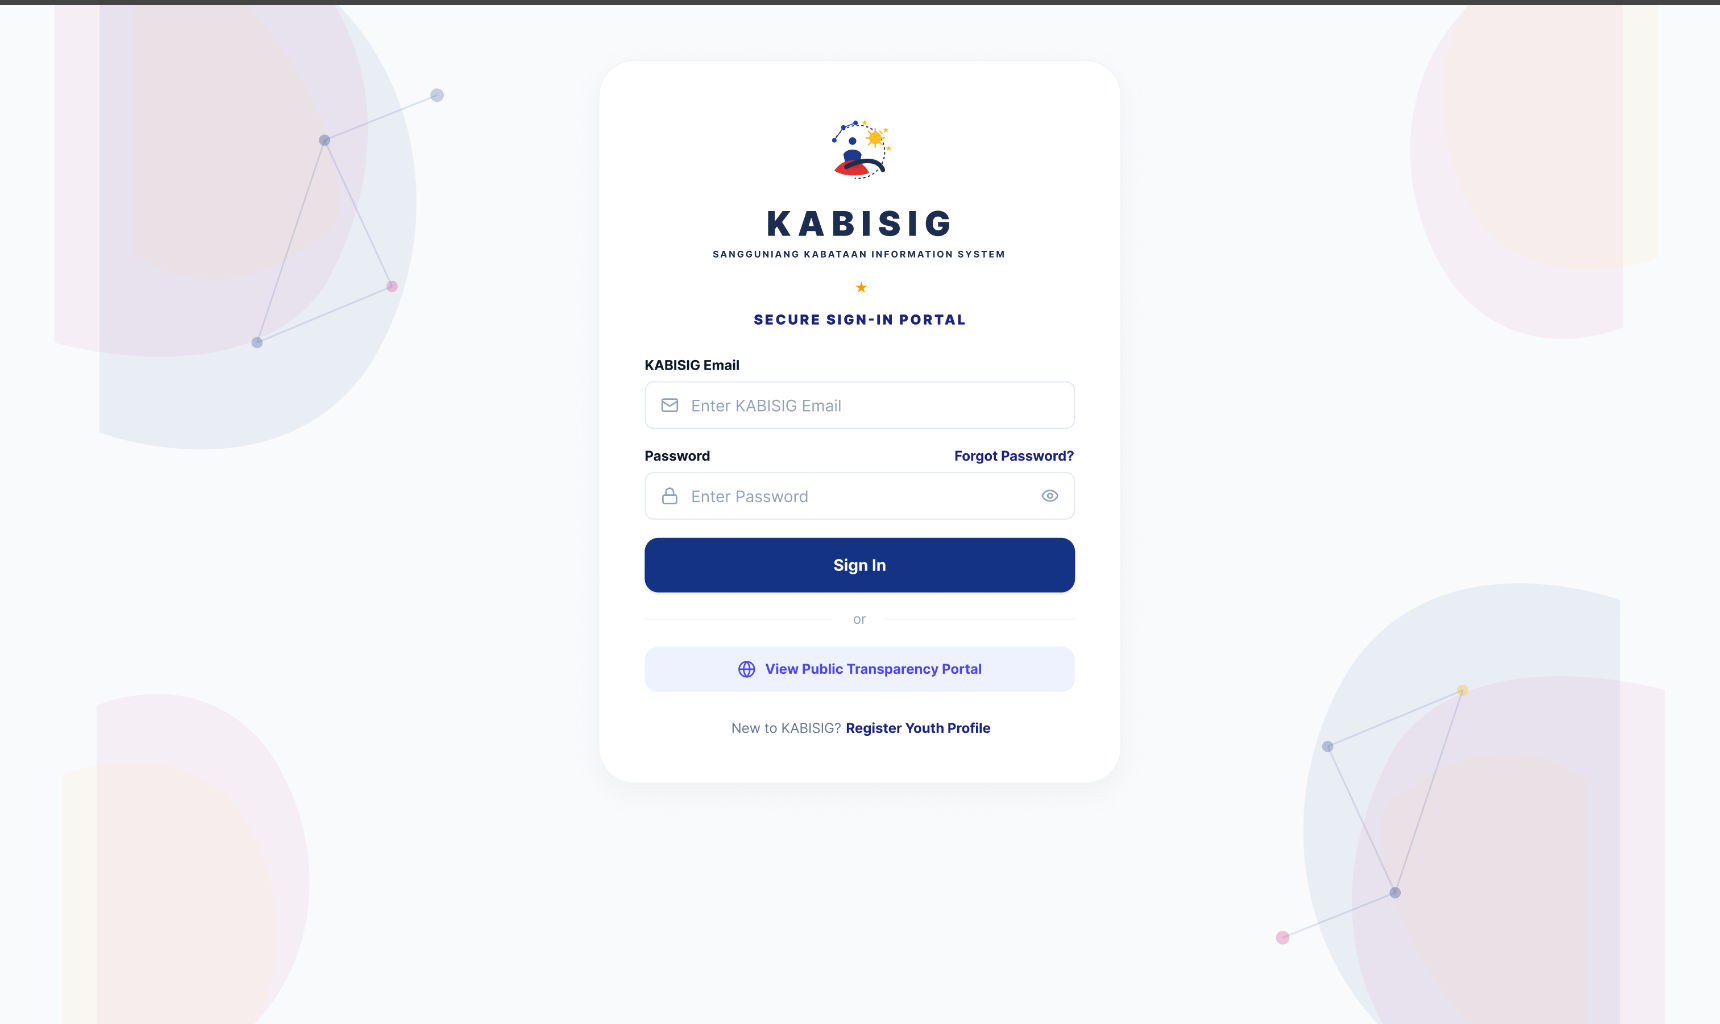
\includegraphics[width=0.45\textwidth]{figures/landing_page.png}
\caption{Public Transparency Portal and Landing Page (Sample Data)}
\label{fig:public_screens}
\end{figure}

\hspace*{\parindent} The authentication flow includes the Secure Sign-In Portal, Create Profile page, and Mandatory Password Change screen. Users are required to change temporary passwords upon first login, ensuring account security. The sign-in portal provides options for both registered users and public access to transparency data.\vspace{5mm}

\begin{figure}[H]
\centering
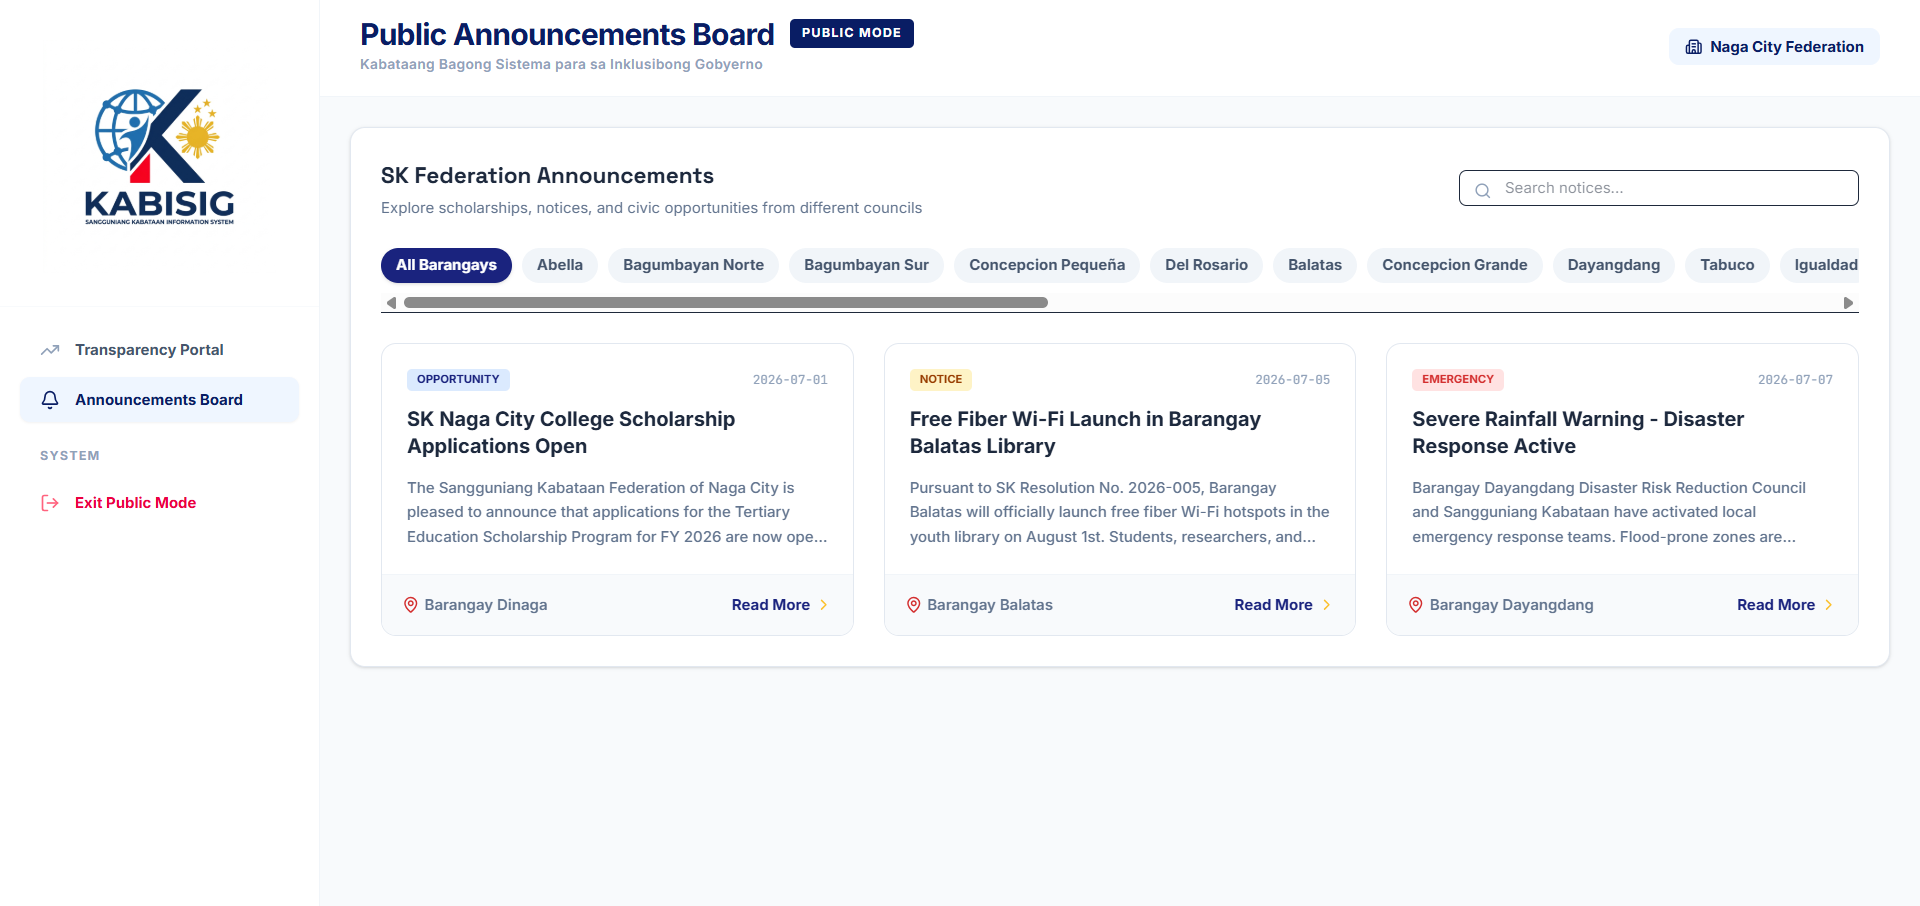
\includegraphics[width=0.30\textwidth]{figures/transparency_portal2.png}
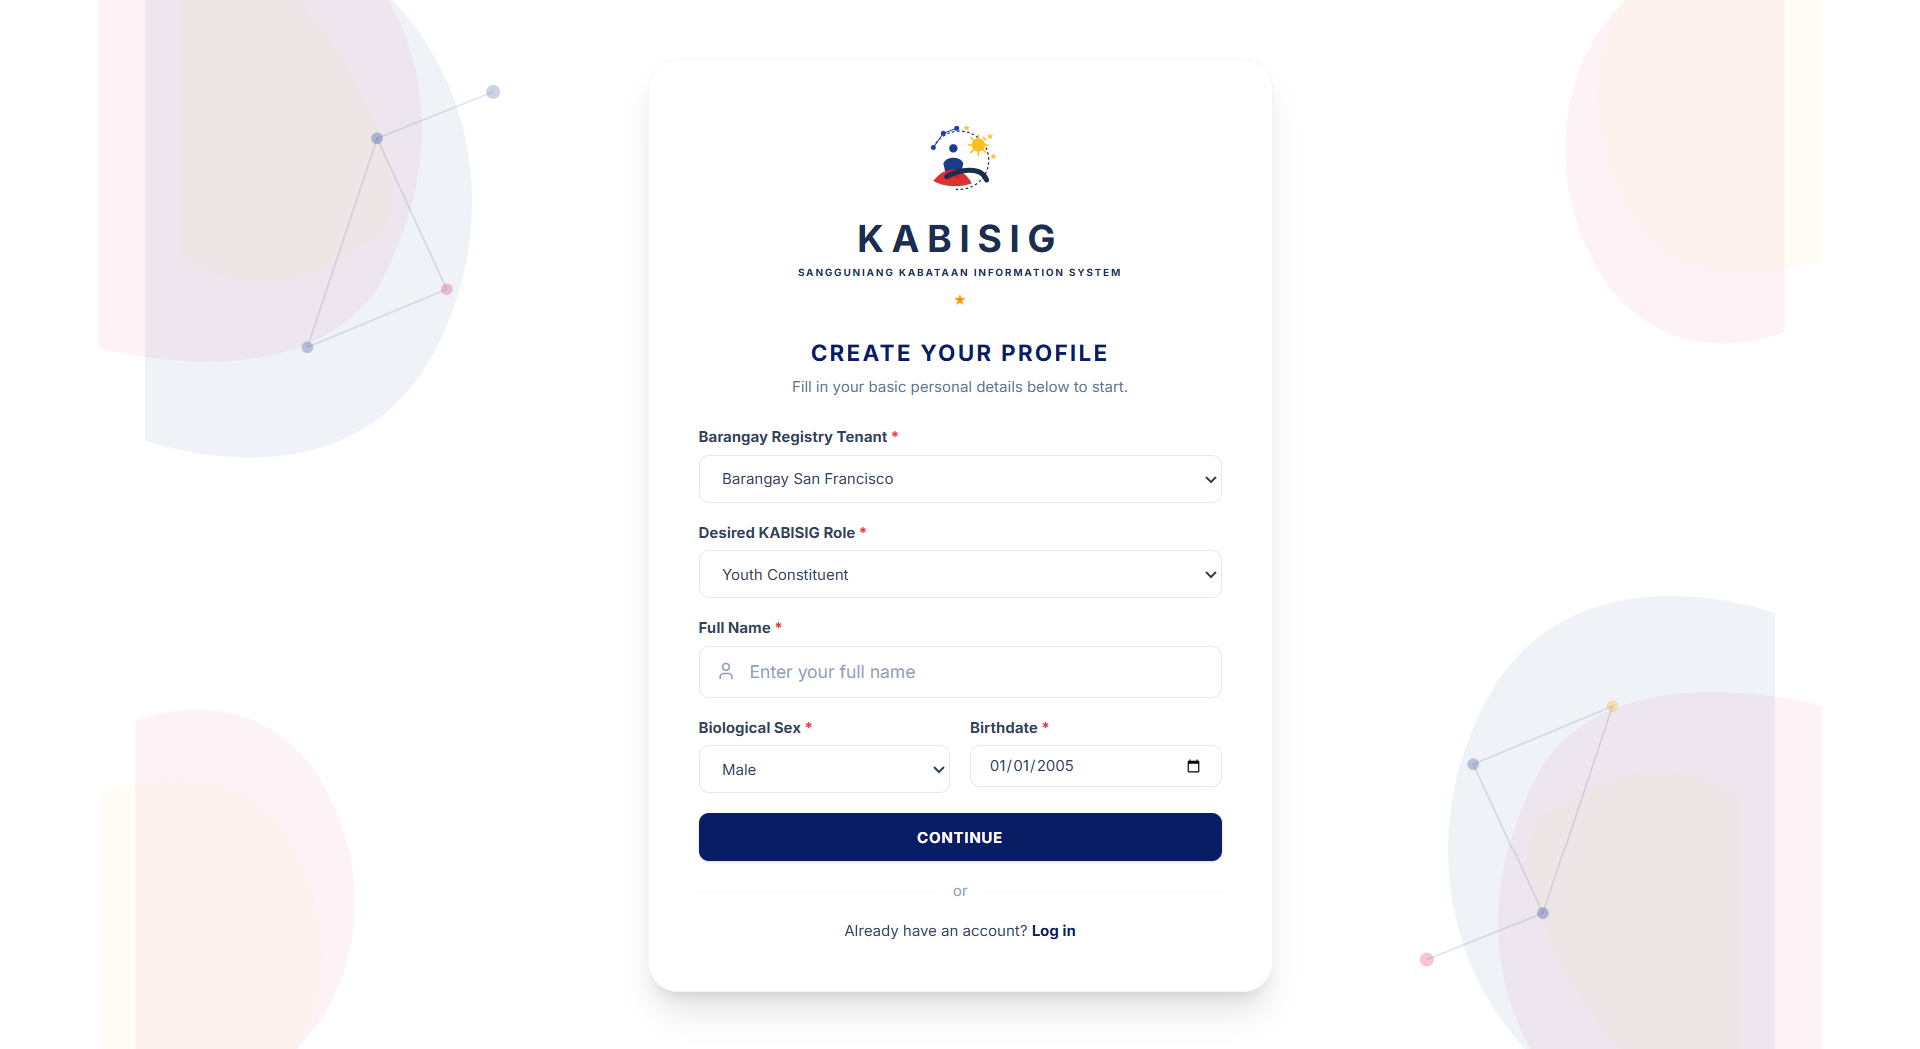
\includegraphics[width=0.30\textwidth]{figures/create_profile.png}
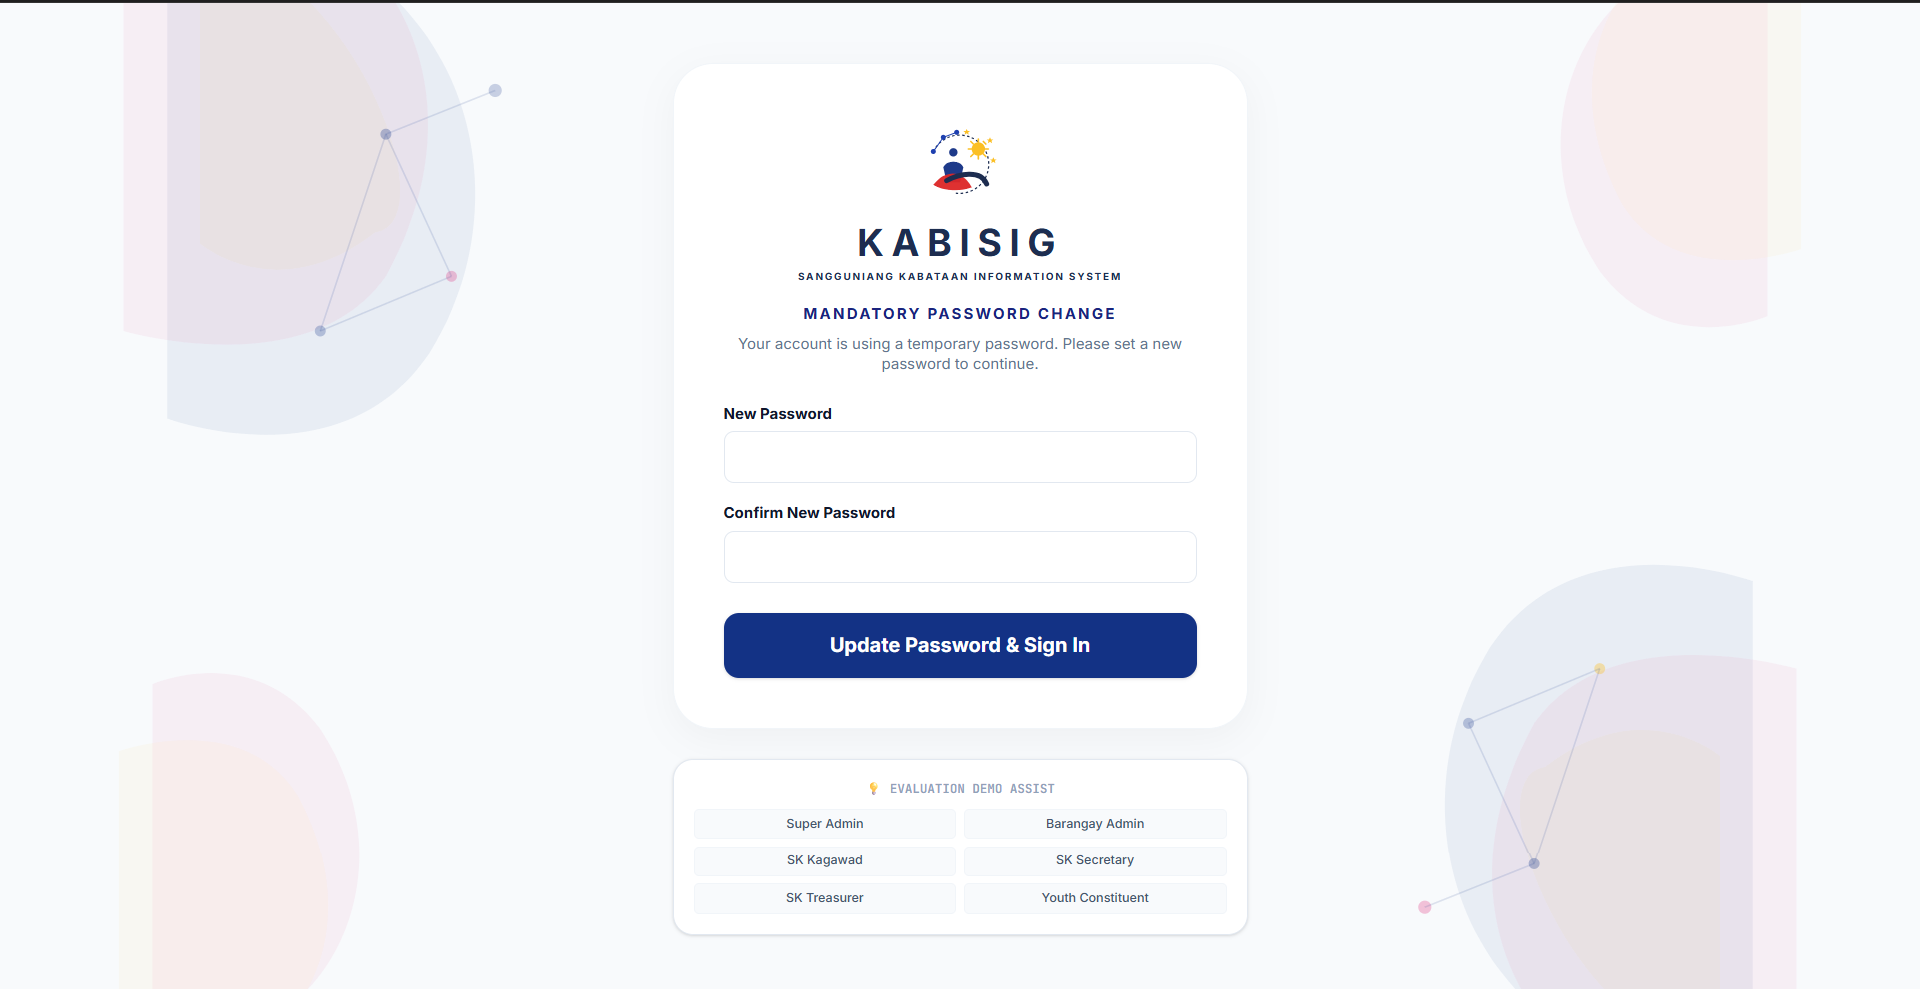
\includegraphics[width=0.30\textwidth]{figures/password_change.png}
\caption{Authentication Screens: Sign-In Portal, Create Profile, and Password Change (Sample Data)}
\label{fig:auth_screens}
\end{figure}

\subsubsection{Super Administrator Screens}

\hspace*{\parindent} The Super Administrator (SK Federation President) dashboard provides a comprehensive overview of all 27 barangays in Naga City. The Federation Dashboard displays key metrics including total barangays, total youth, active programs, and total budget. The welcome screen greets the SK Federation President with a personalized message and role badge, providing quick access to system-wide statistics and management tools.\vspace{5mm}

\begin{figure}[H]
\centering
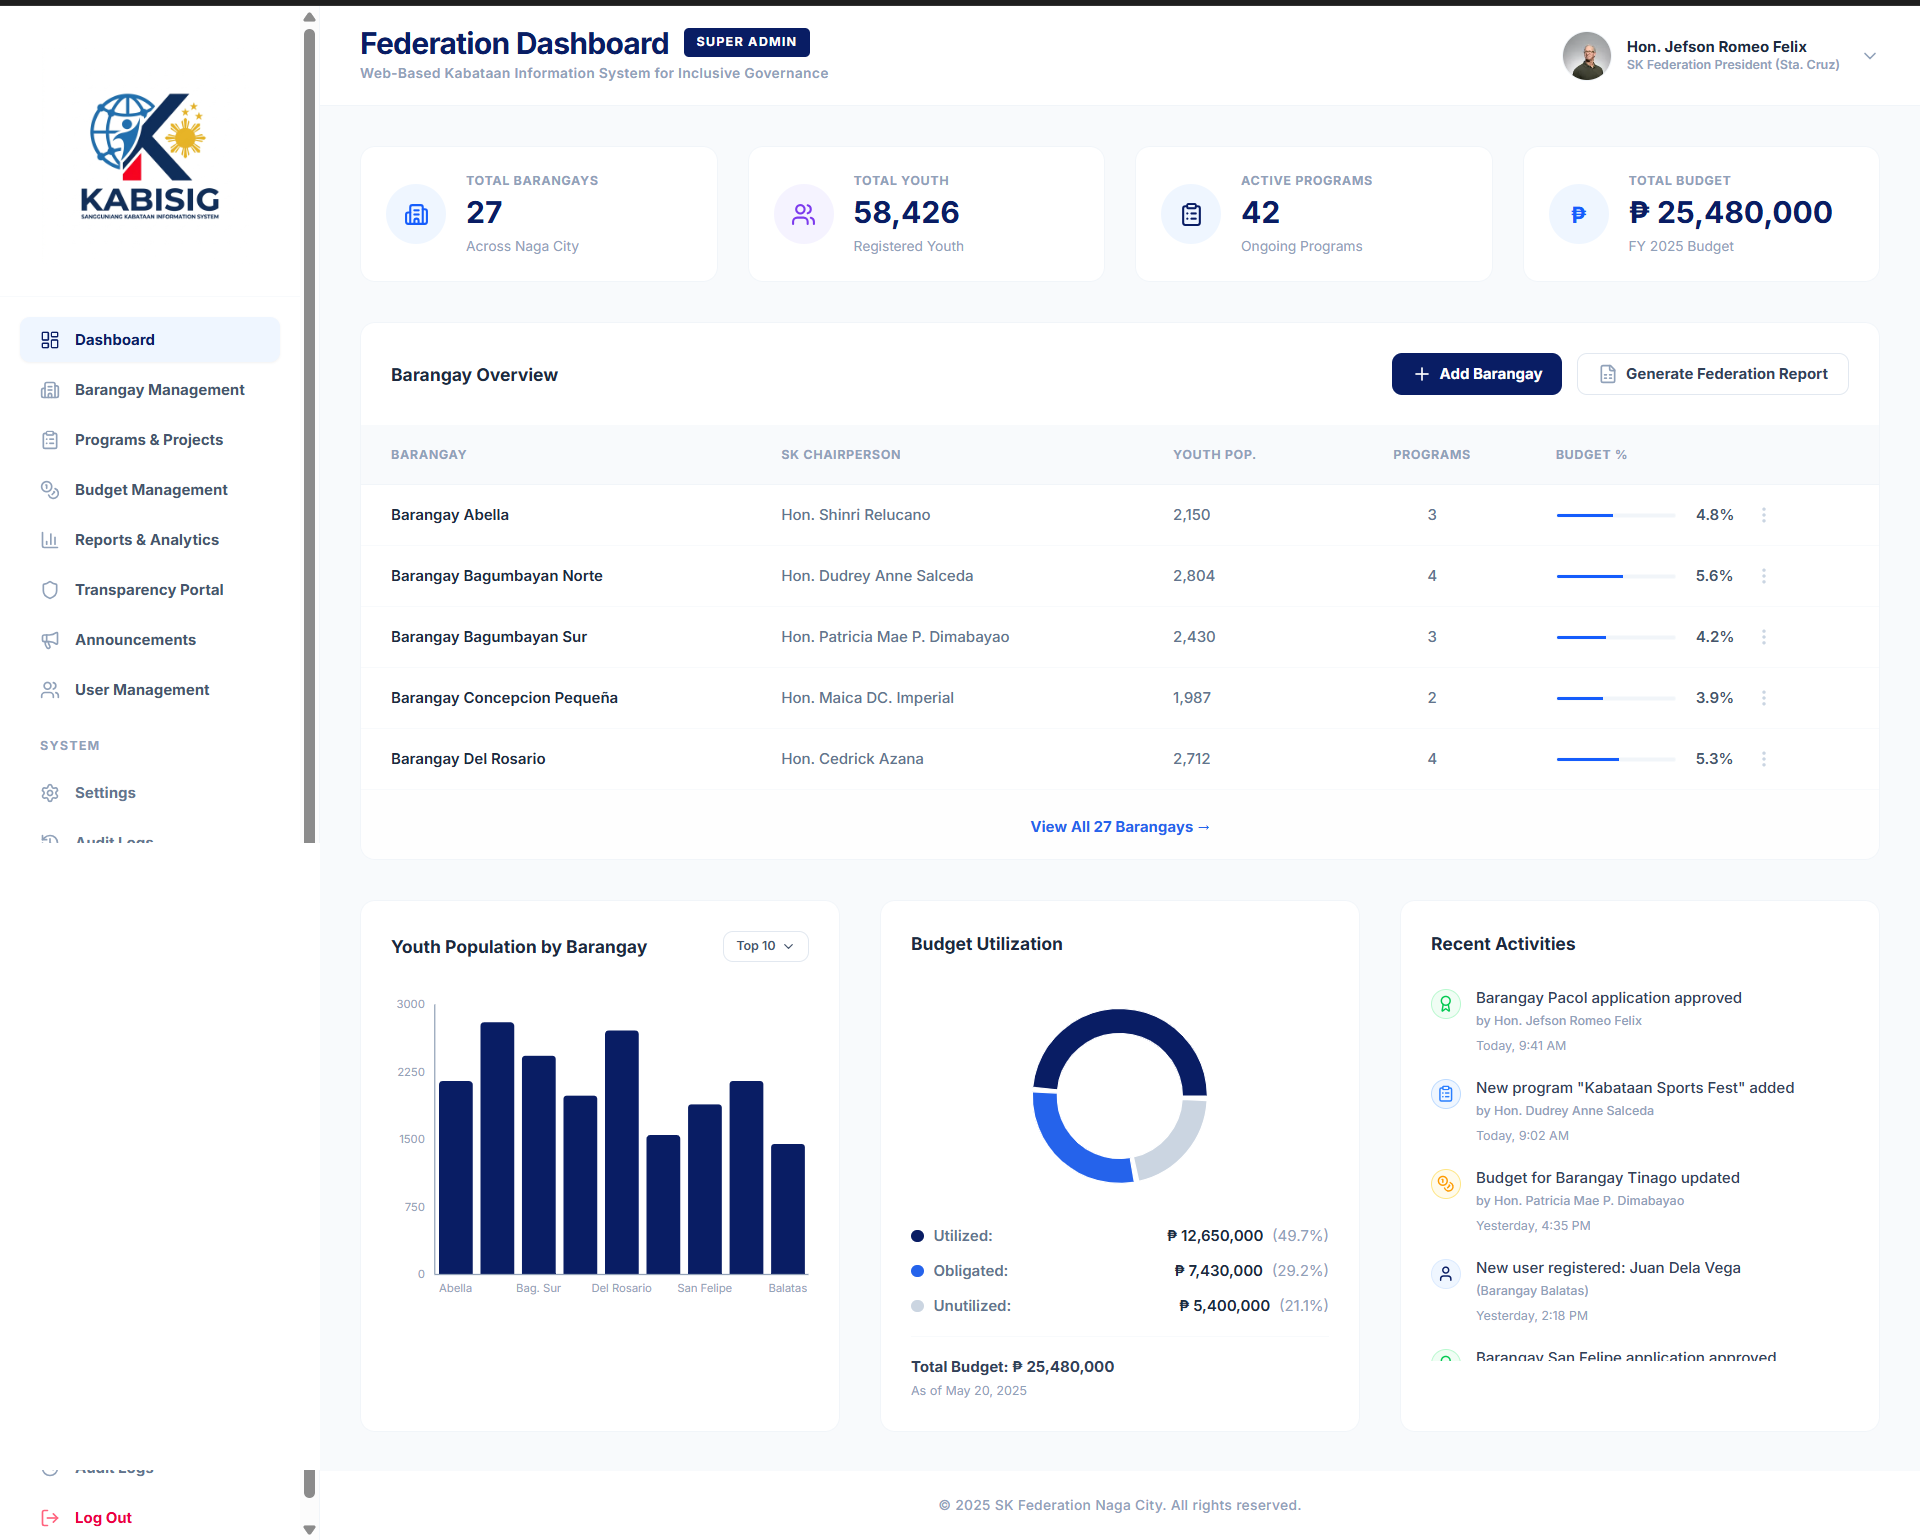
\includegraphics[width=0.45\textwidth]{figures/super_admin_dashboard.png}
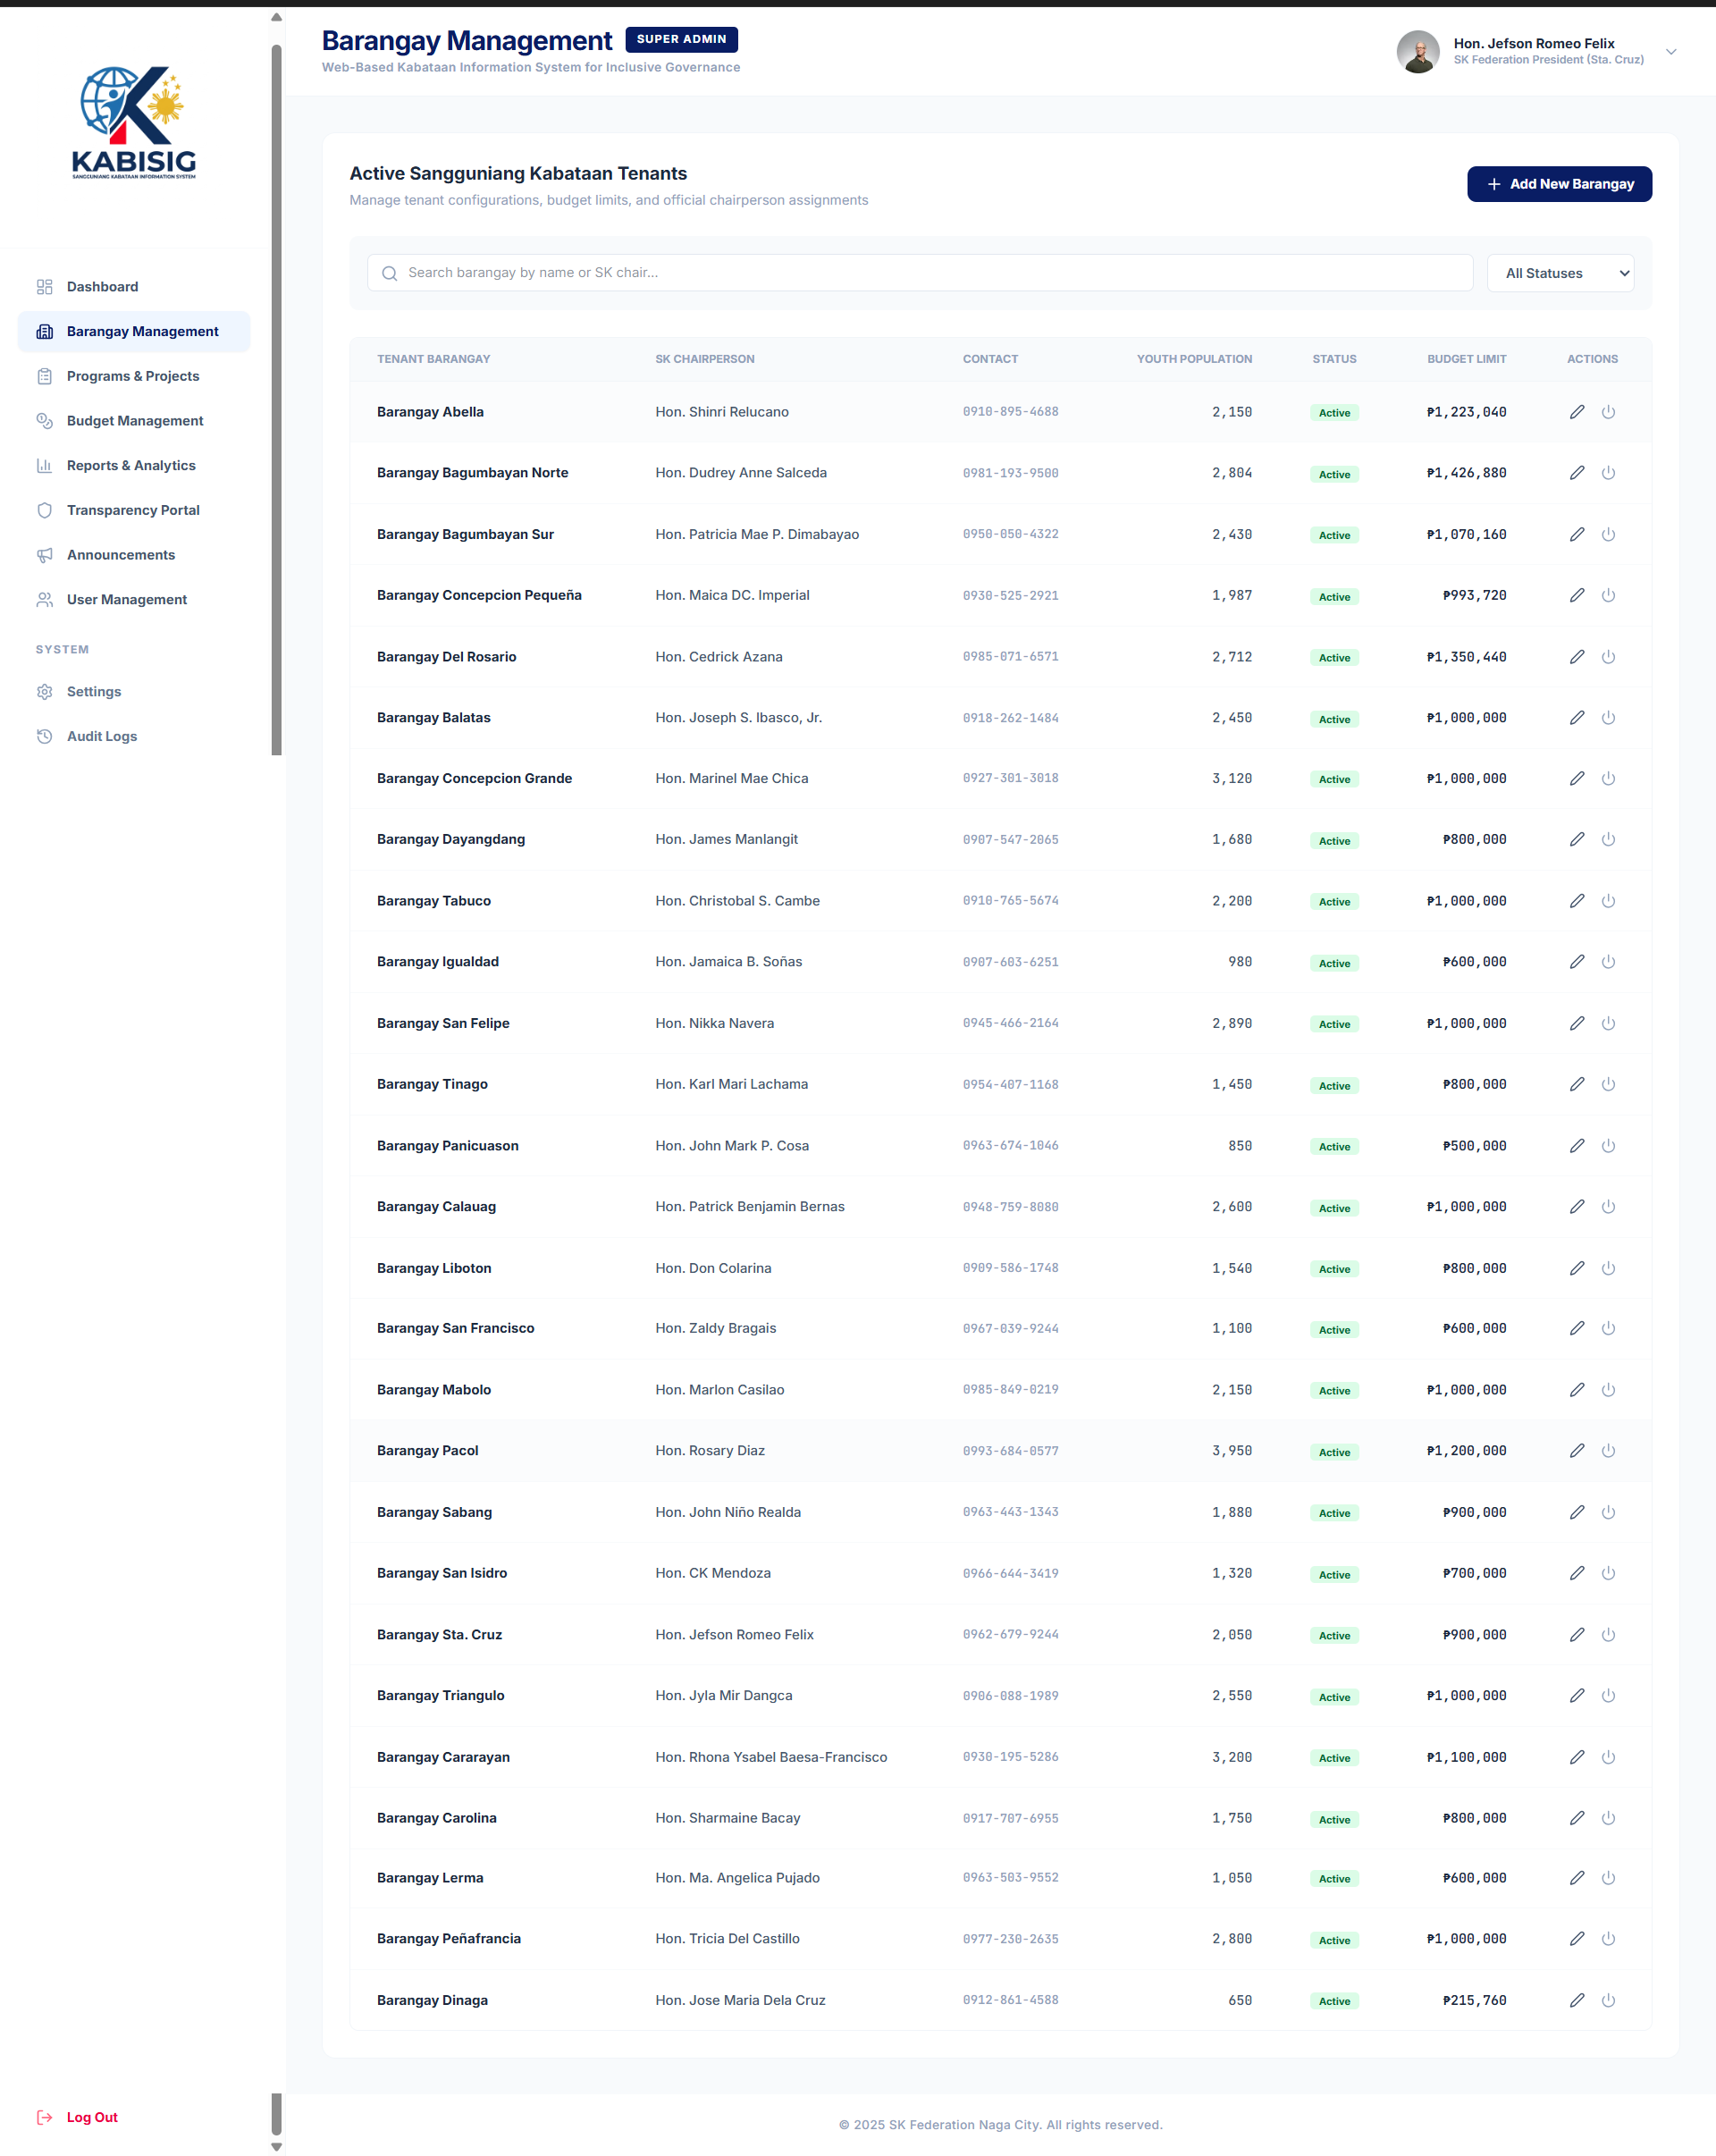
\includegraphics[width=0.45\textwidth]{figures/barangay_overview.png}
\caption{Super Administrator Federation Dashboard and Barangay Overview (Sample Data)}
\label{fig:super_admin}
\end{figure}

\hspace*{\parindent} The barangay overview lists each barangay with its SK Chairperson, youth population, program count, and budget utilization percentage. The dashboard also includes visual analytics such as Youth Population by Barangay charts and Budget Utilization distribution. Recent activities are logged for monitoring purposes, including barangay application approvals, program additions, and budget updates.\vspace{5mm}

\subsubsection{Barangay Administrator Screens}

\hspace*{\parindent} The Barangay Admin Dashboard provides SK Chairpersons with a focused view of their specific barangay's statistics and activities. Key metrics include youth population, active programs, total budget, and pending approvals. Quick action buttons provide access to Create Program, View Registrations, and Manage Documents functionalities.\vspace{5mm}

\begin{figure}[H]
\centering
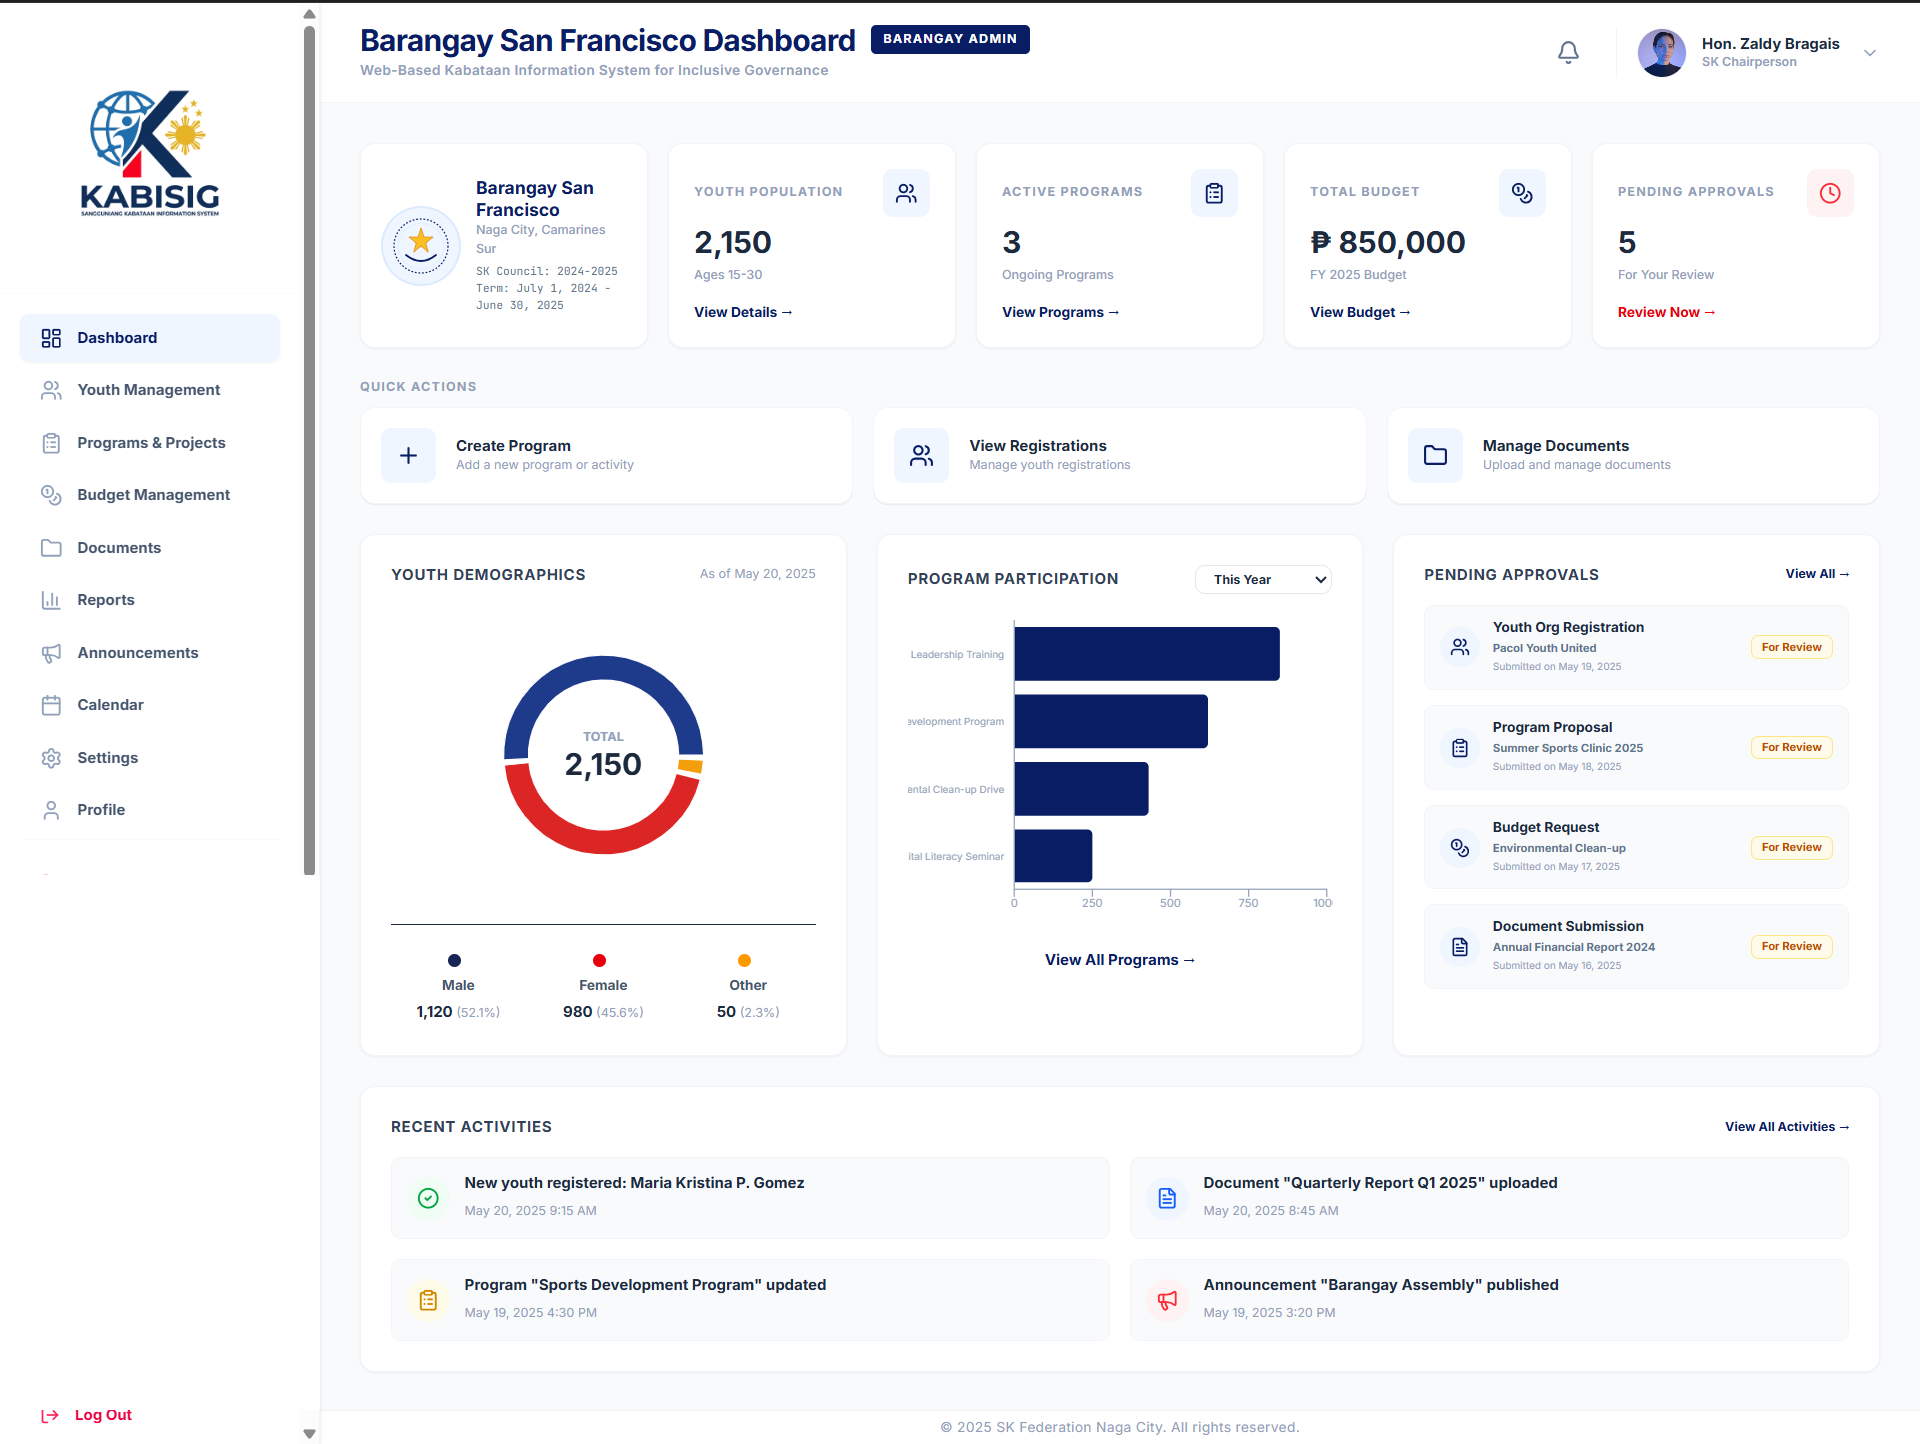
\includegraphics[width=0.45\textwidth]{figures/barangay_admin_dashboard.png}
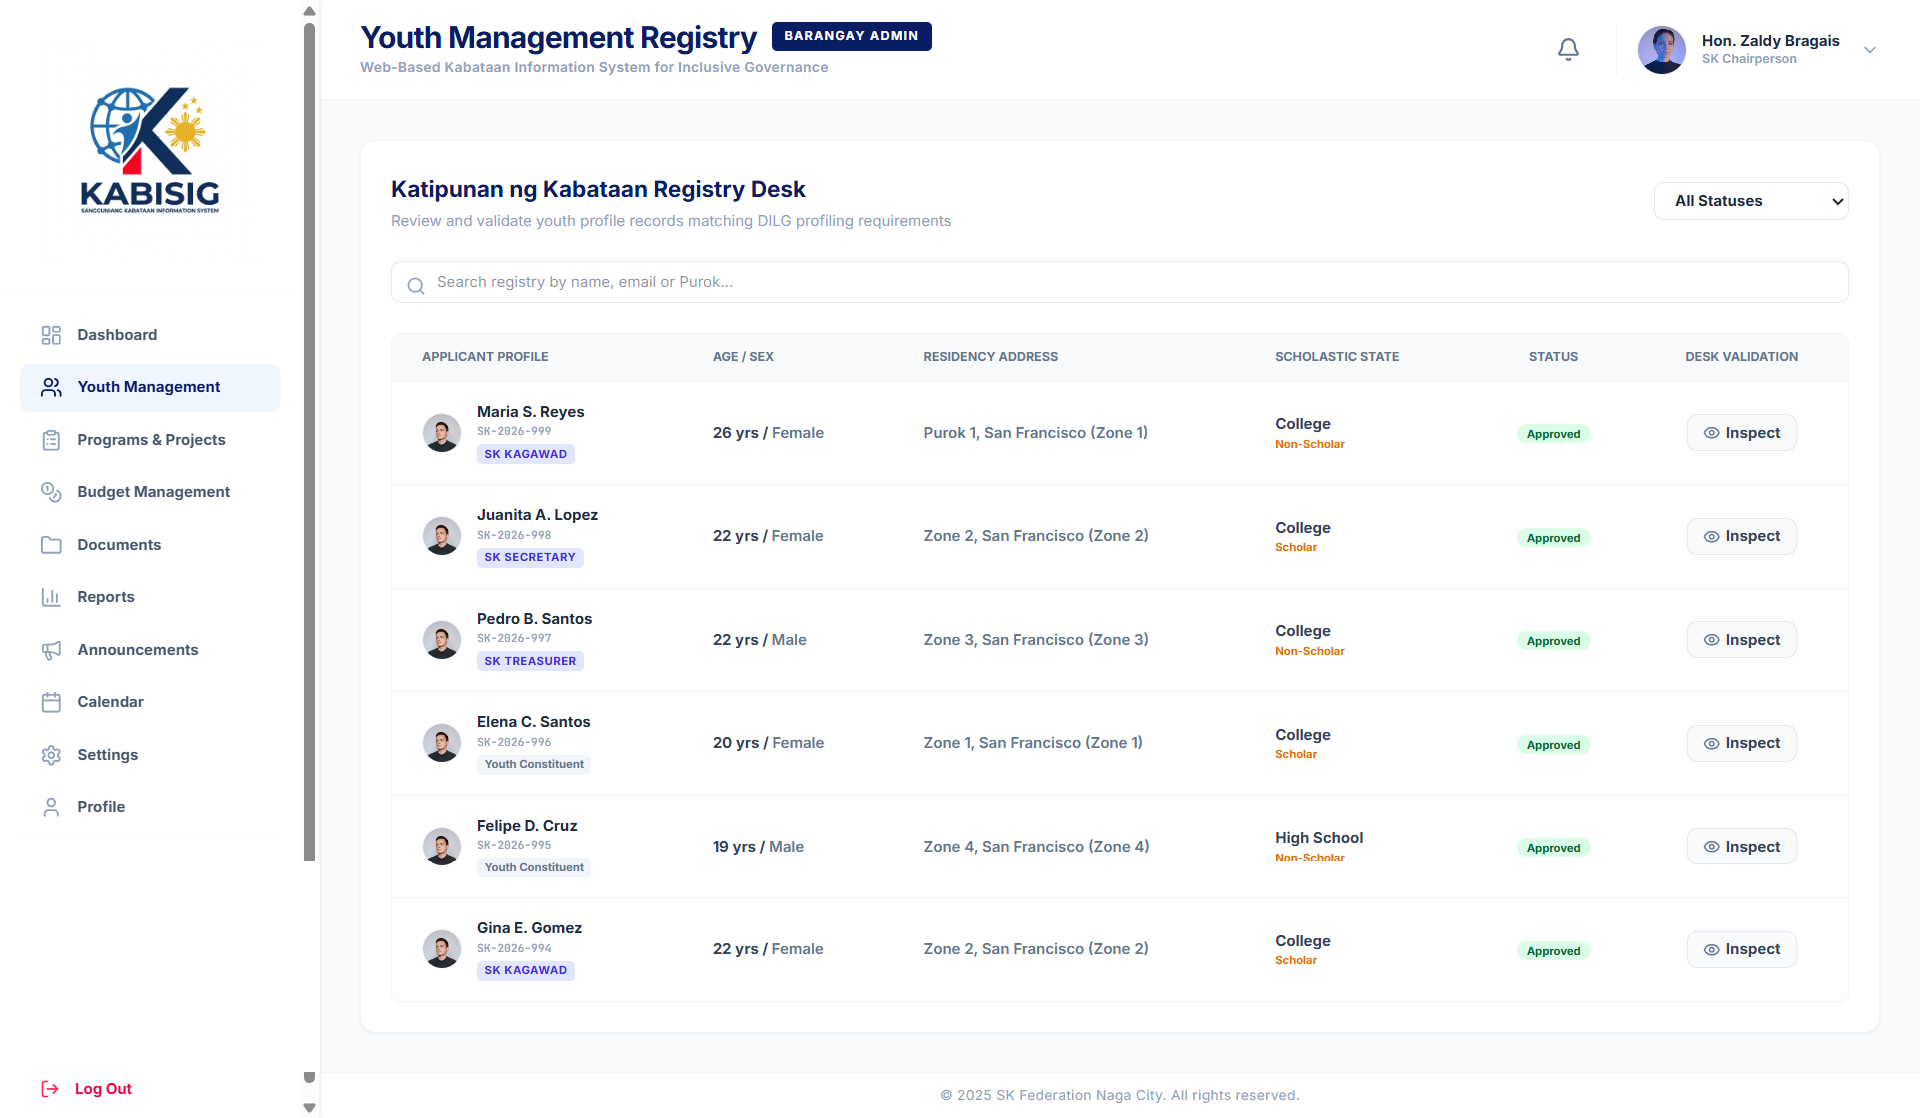
\includegraphics[width=0.45\textwidth]{figures/youth_management.png}
\caption{Barangay Admin Dashboard and Youth Management (Sample Data)}
\label{fig:barangay_admin}
\end{figure}

\hspace*{\parindent} The Youth Management module allows Barangay Admins to view and approve youth registrations, generate Digital Youth IDs, and manage beneficiary records. Pending registrations are displayed with approve/reject actions, ensuring only verified residents gain access to SK services.\vspace{5mm}

\hspace*{\parindent} The Facebook Page Synchronization module enables Barangay Admins to connect KABISIG with their official SK Facebook page. This feature ensures consistent public communication by automatically synchronizing announcements, program postings, and updates between KABISIG and Facebook. The Social Sync dashboard provides a comprehensive social announcements ledger with status tracking for all posts.\vspace{5mm}

\begin{figure}[H]
\centering
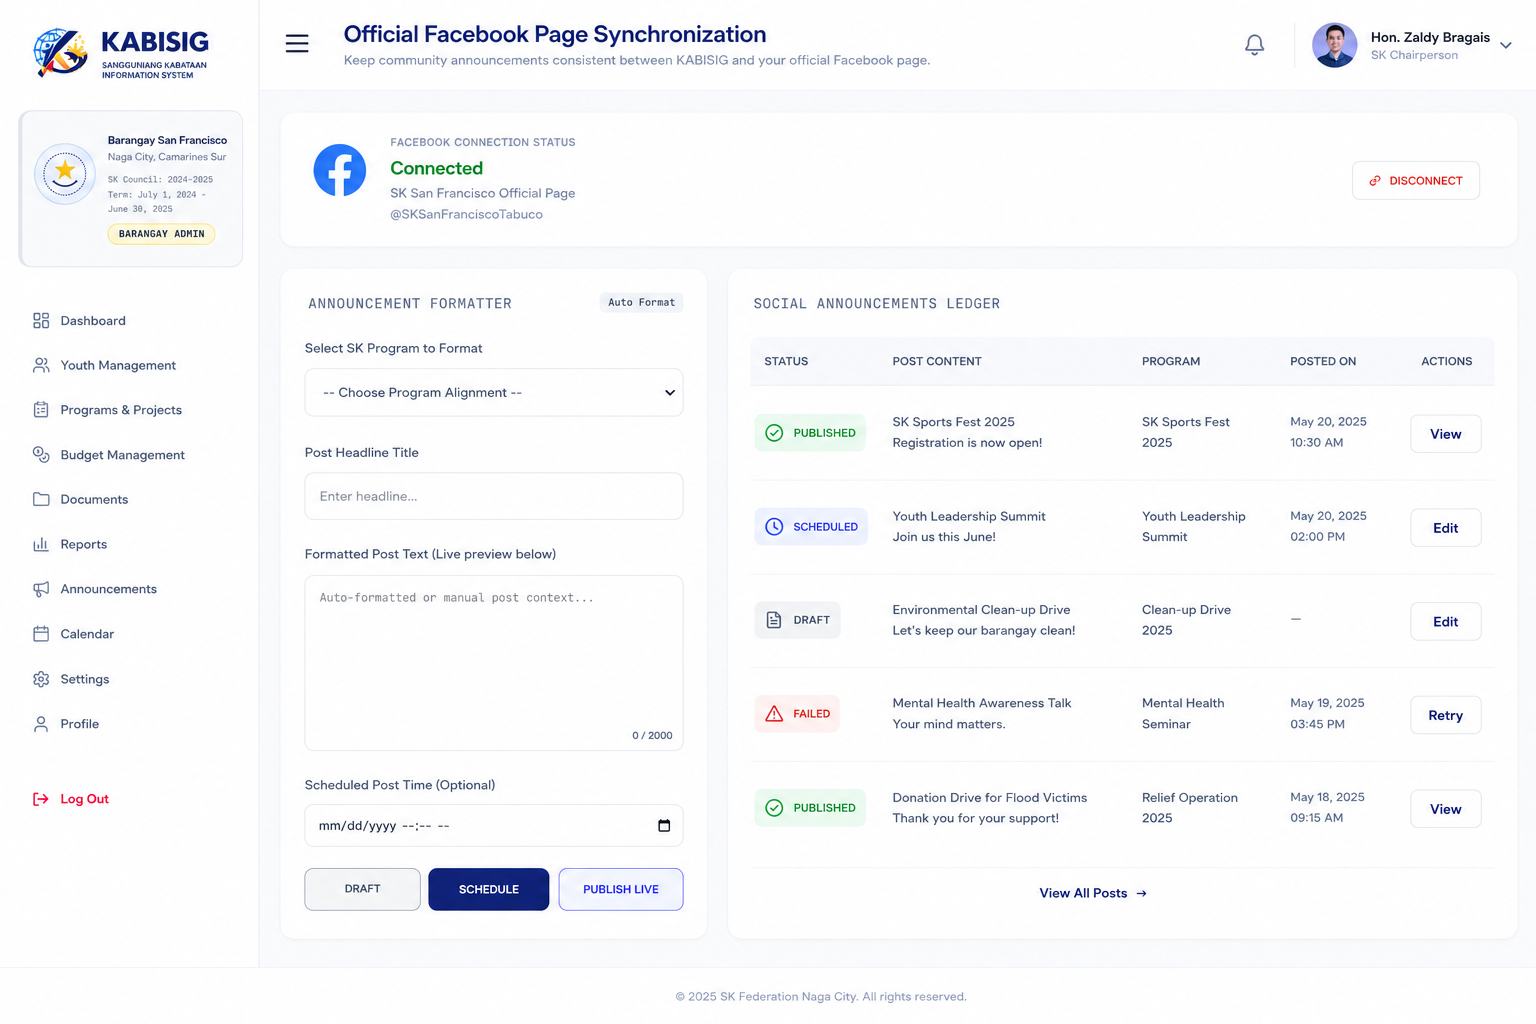
\includegraphics[width=0.45\textwidth]{figures/facebook_sync.png}
\caption{Barangay Admin Facebook Page Synchronization (Sample Data)}
\label{fig:facebook_sync}
\end{figure}

\hspace*{\parindent} The Social Sync interface includes the following key features:\vspace{3mm}

\begin{itemize}
    \item \textbf{Announcement Formatter:} Users can select SK programs to format, enter post headlines, and generate auto-formatted Facebook post content with live preview.
    \item \textbf{Post Status Tracking:} Each social media post is tracked with status badges (Published, Scheduled, Draft, Failed) for easy monitoring and management.
    \item \textbf{Social Announcements Ledger:} A comprehensive ledger displays all posts with their status, content, associated program, and posting date. Actions include View, Edit, and Retry for failed posts.
    \item \textbf{Scheduled Posting:} Users can schedule posts for future publication with configurable date and time.
    \item \textbf{Post Statistics:} Summary cards show the count of Scheduled, Draft, and Published posts for quick overview.
\end{itemize}

\vspace{5mm}

\subsubsection{SK Kagawad Screens}

\hspace*{\parindent} The SK Kagawad workspace includes the Attendance Tracking module with QR scanner functionality. The scanner uses the device's camera via WebRTC and the Web Barcode Detection API, allowing officials to scan youth QR codes for attendance marking. Manual entry mode is also available as a backup option.\vspace{5mm}

\begin{figure}[H]
\centering
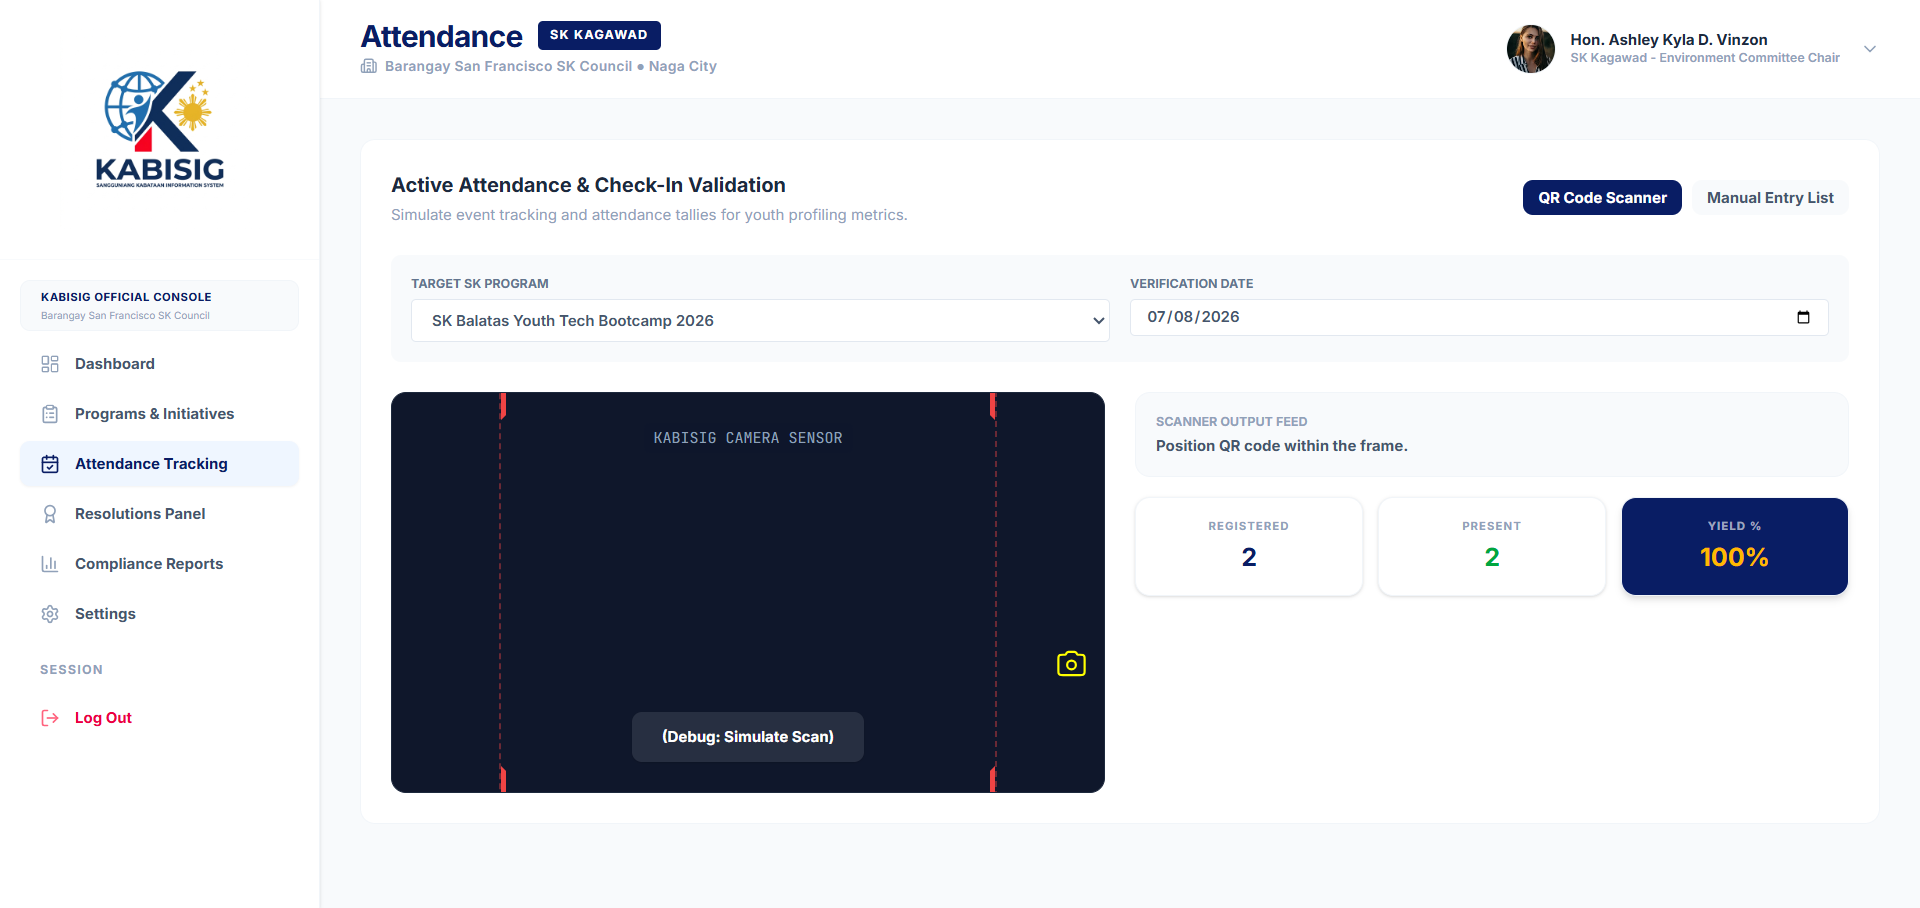
\includegraphics[width=0.45\textwidth]{figures/kagawad_attendance.png}
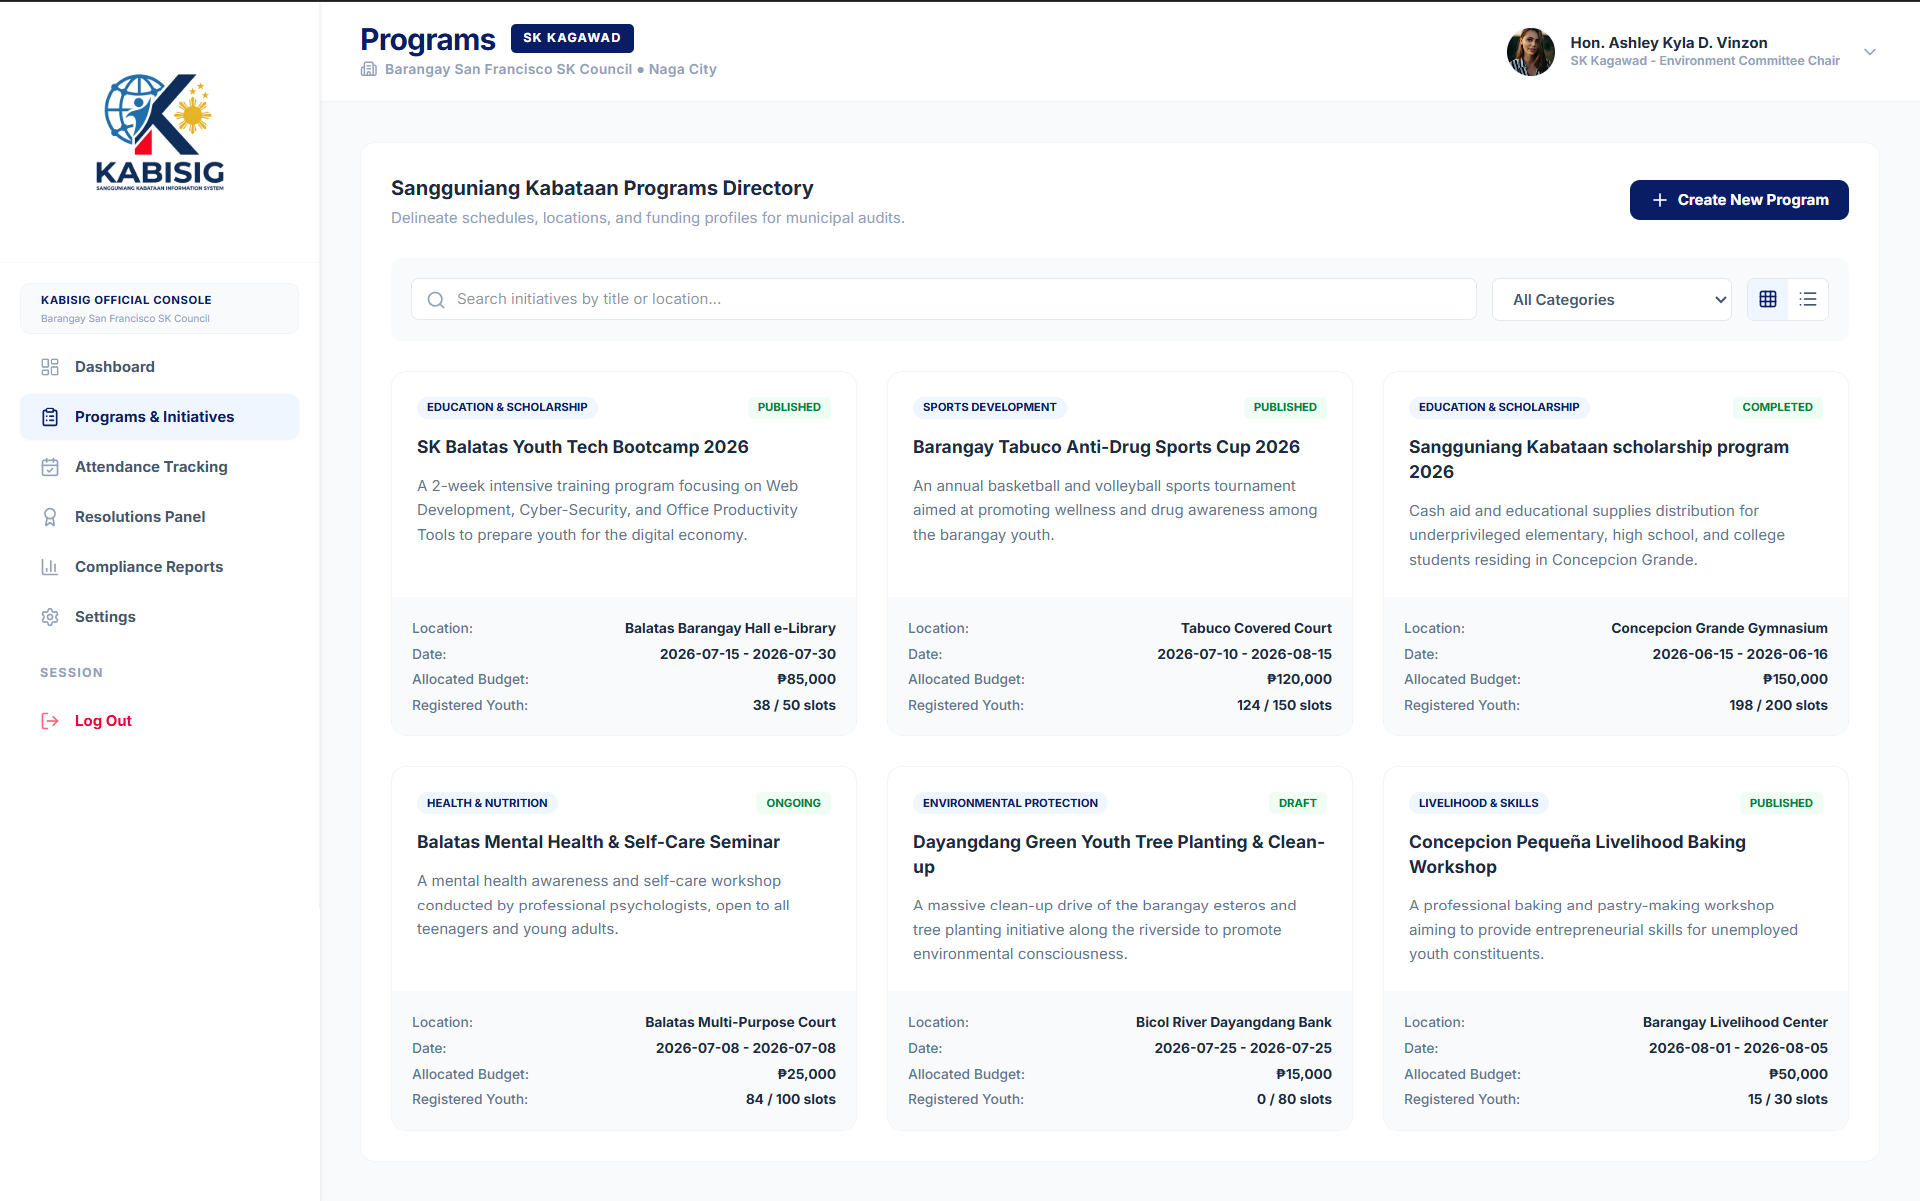
\includegraphics[width=0.45\textwidth]{figures/program_management.png}
\caption{SK Kagawad Attendance Tracking and Program Management (Sample Data)}
\label{fig:kagawad}
\end{figure}

\hspace*{\parindent} The Program Management screen displays program cards with key information including title, date, status, budget, and registrations. SK Kagawad can create, edit, and manage programs, with calendar view and list view options for flexible program tracking.\vspace{5mm}

\subsubsection{SK Secretary Screens}

\hspace*{\parindent} The SK Secretary Document Repository provides centralized document management for governance documents. Users can upload documents, categorize them by type (Resolutions, Vouchers, Reports, Budget), and track document status (Approved, Pending, Draft). The search and filter functionality enables efficient document retrieval.\vspace{5mm}

\begin{figure}[H]
\centering
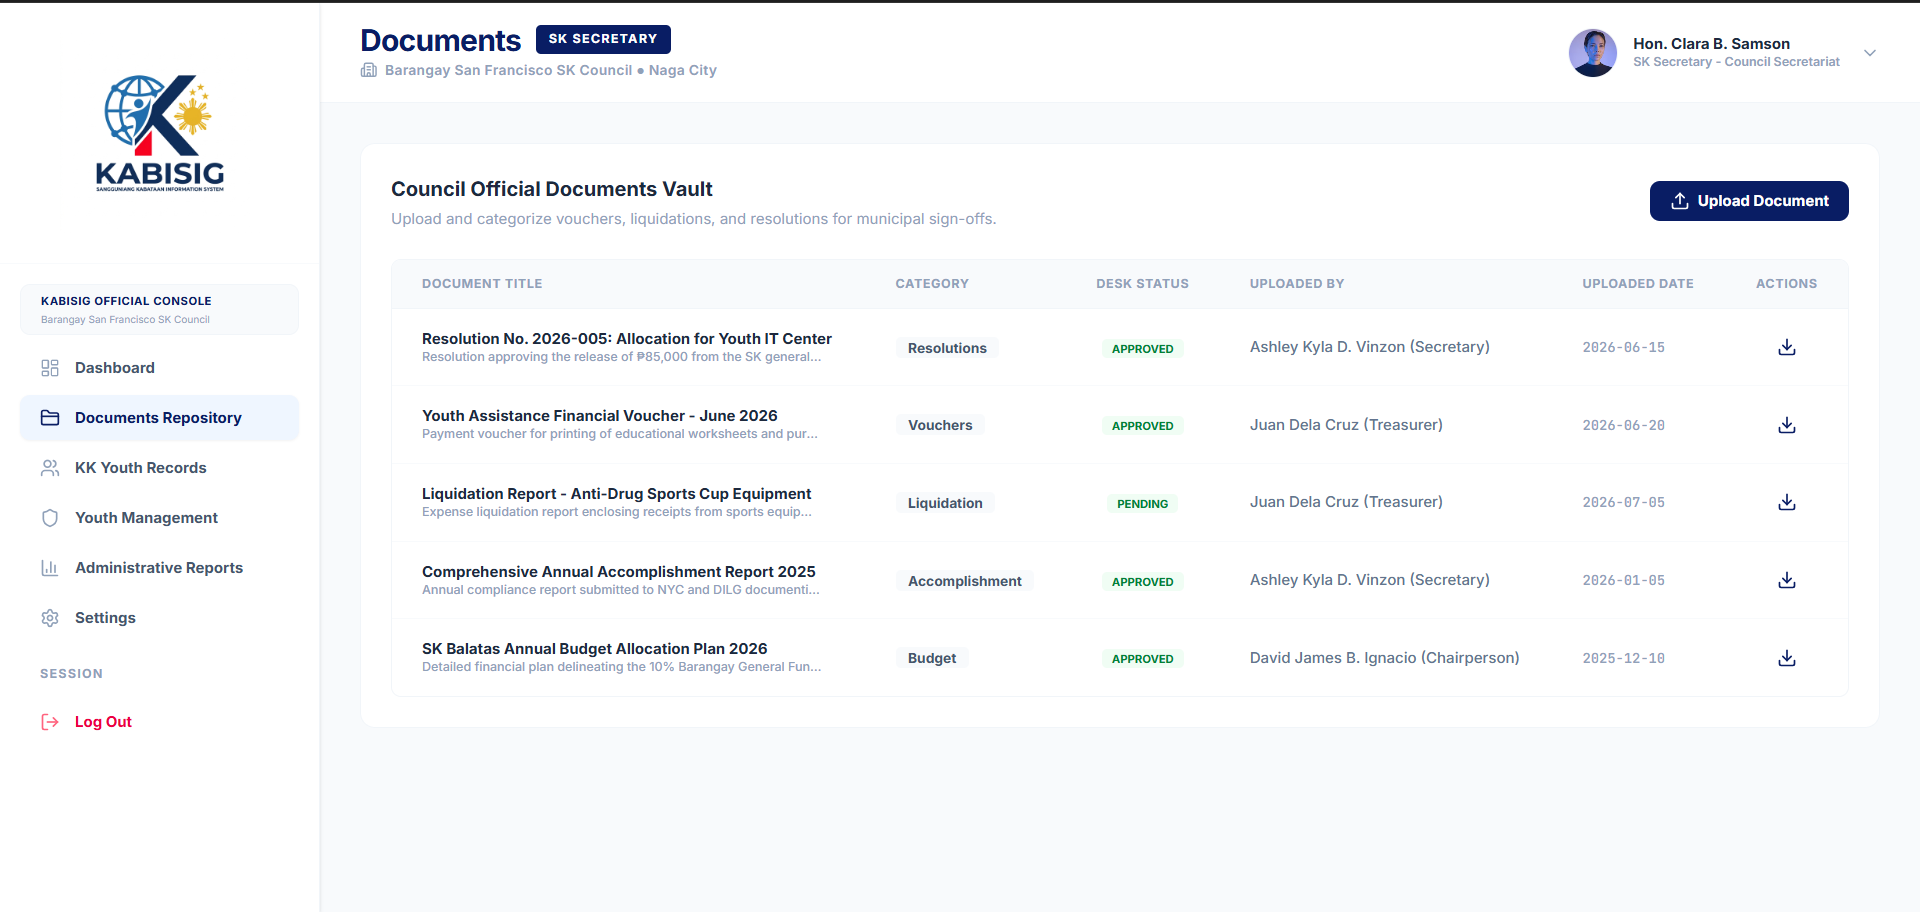
\includegraphics[width=0.45\textwidth]{figures/document_repository.png}
\caption{SK Secretary Document Repository (Sample Data)}
\label{fig:secretary}
\end{figure}

\hspace*{\parindent} Each document card displays the title, description, status badge, and date. Status badges use color coding: Approved (Green), Pending (Yellow), and Draft (Gray). Document actions include View, Download, Edit, and Route for Approval.\vspace{5mm}

\subsubsection{SK Treasurer Screens}

\hspace*{\parindent} The SK Treasurer Inventory Registry tracks SK council properties and assets. The interface displays property items with category group, quantity, condition, and location information. Users can register new assets and search the inventory.\vspace{5mm}

\begin{figure}[H]
\centering
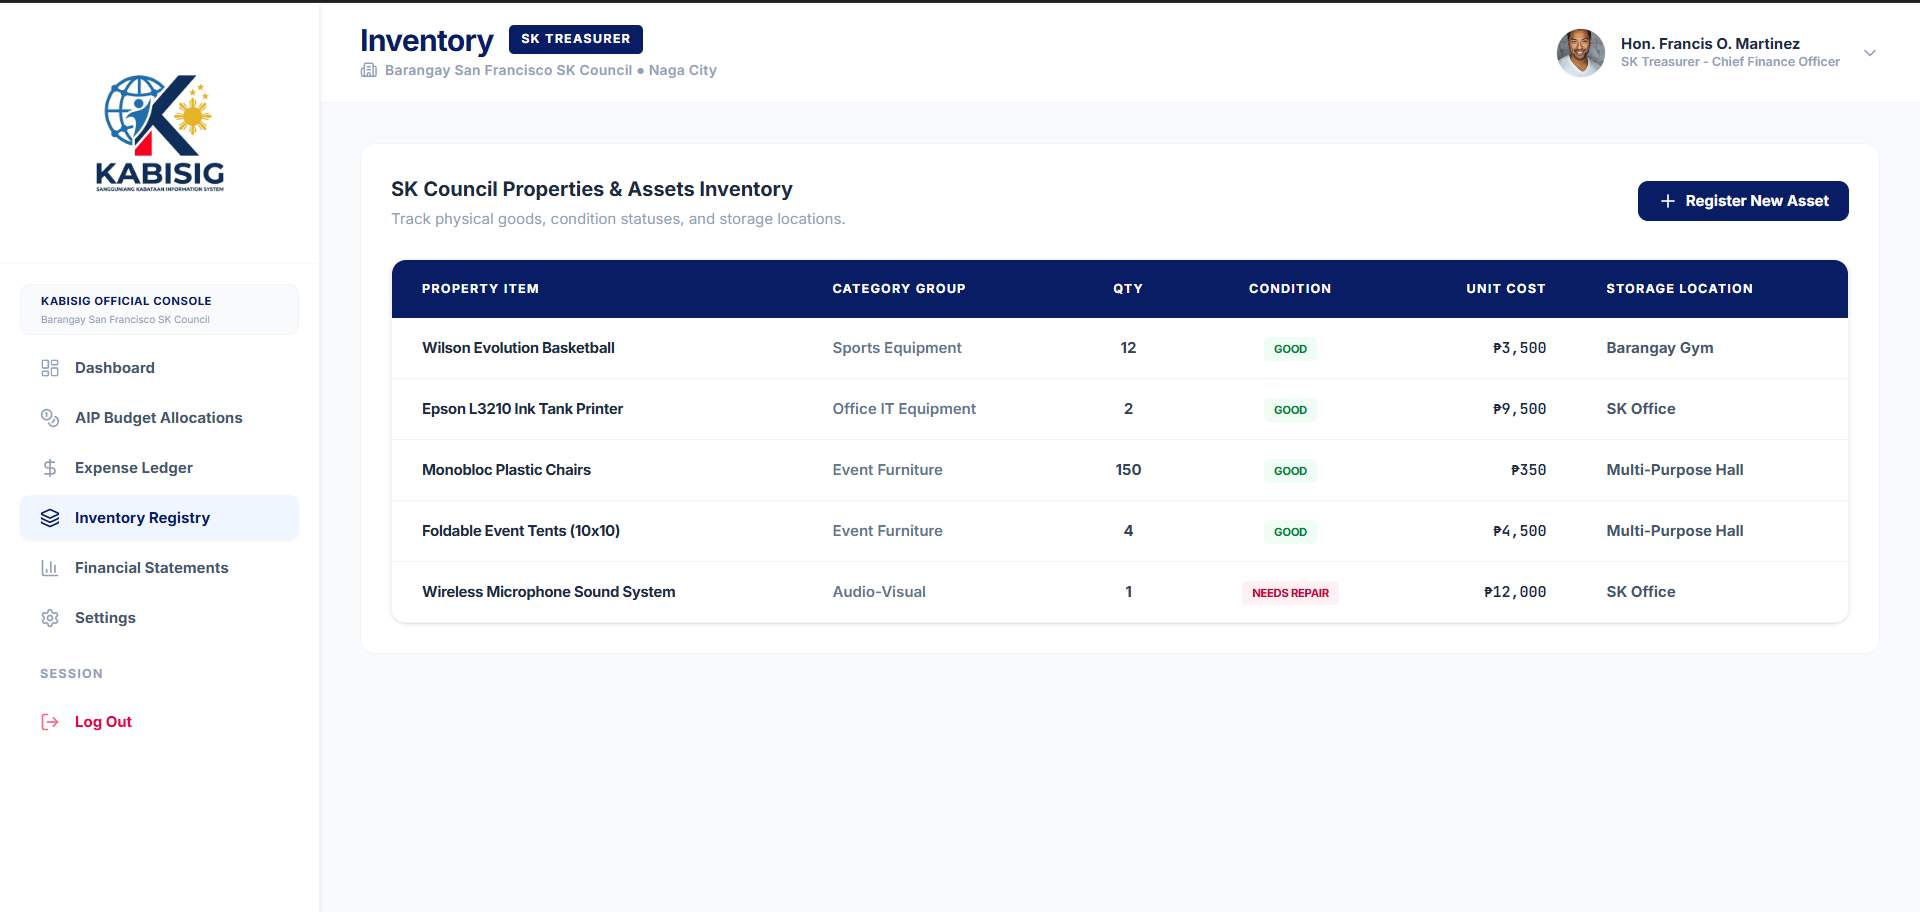
\includegraphics[width=0.45\textwidth]{figures/treasurer_inventory.png}
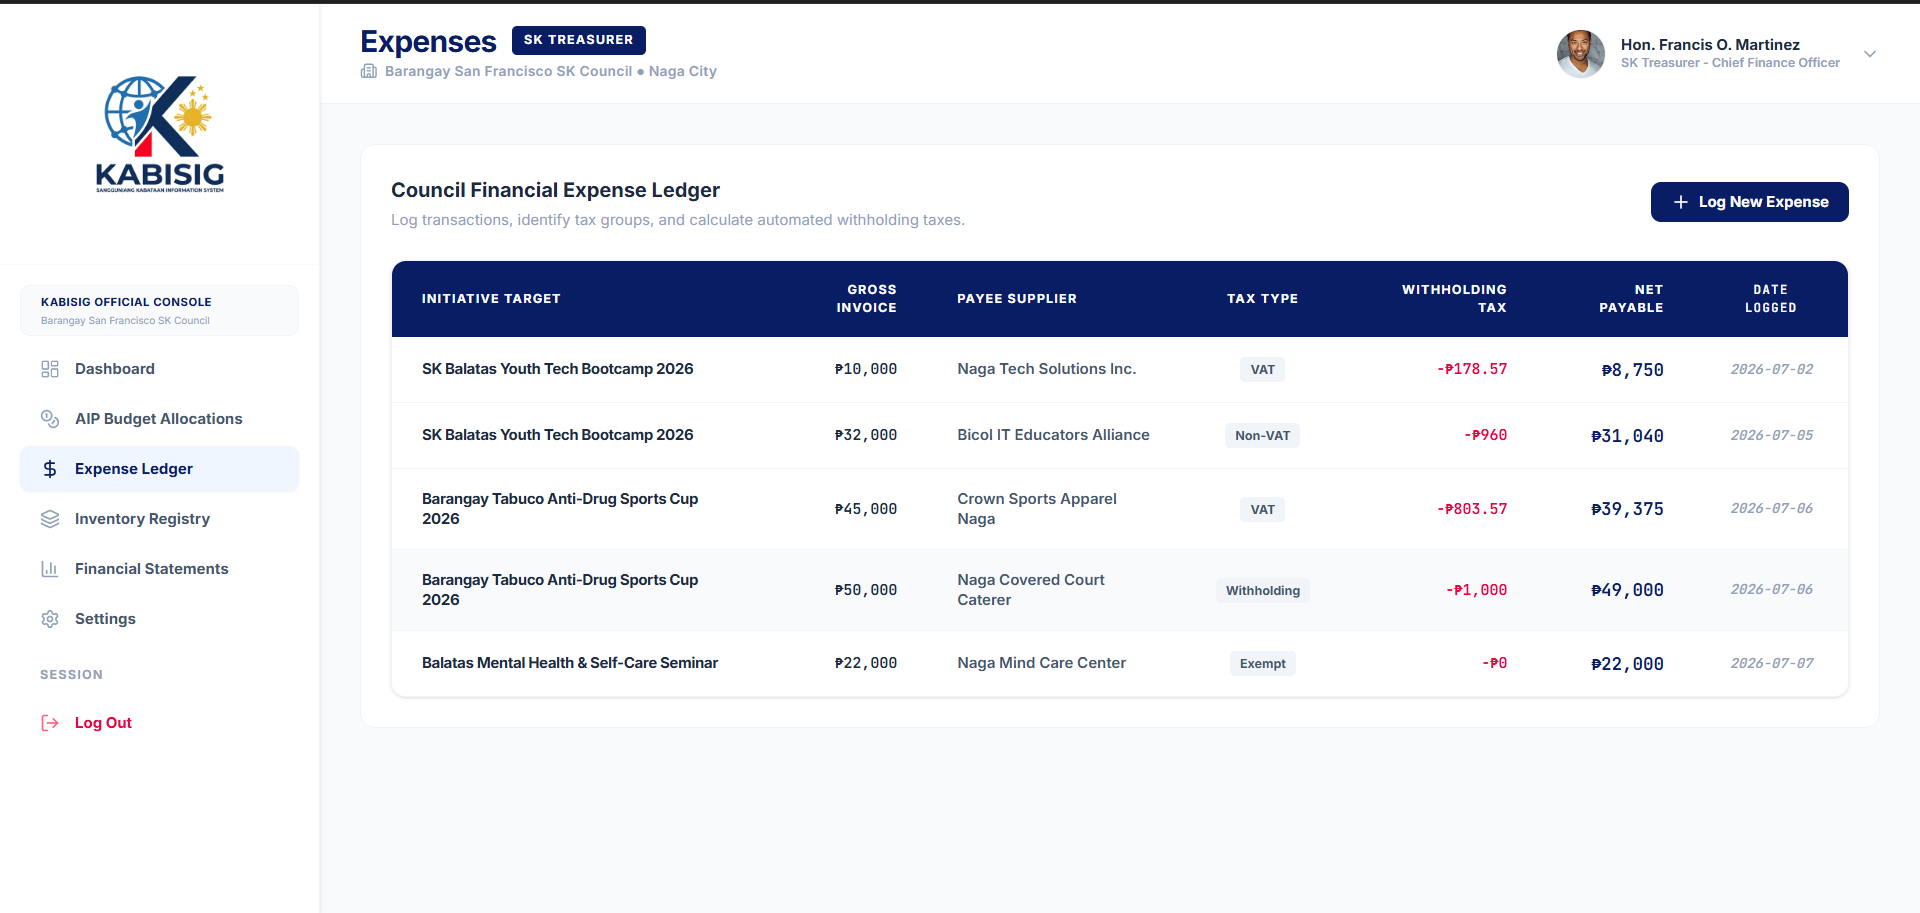
\includegraphics[width=0.45\textwidth]{figures/Expense_management.png}
\caption{SK Treasurer Inventory Registry and Budget Management (Sample Data)}
\label{fig:treasurer}
\end{figure}

\hspace*{\parindent} The Budget Management screen provides financial oversight with automated VAT/Non-VAT computation. Expense items display initiative description, gross amount, tax class, net disbursement, and status. The system automatically generates budget utilization reports and alerts for overspending.\vspace{5mm}

\subsubsection{Youth Constituent Screens}

\hspace*{\parindent} The Youth Dashboard provides a personalized homepage for youth constituents, displaying their Digital Youth ID, key statistics (barangay youth population, ongoing programs, participation count, active polls), and upcoming programs. The Digital Youth ID includes serial number, address, and verification status.\vspace{5mm}

\begin{figure}[H]
\centering
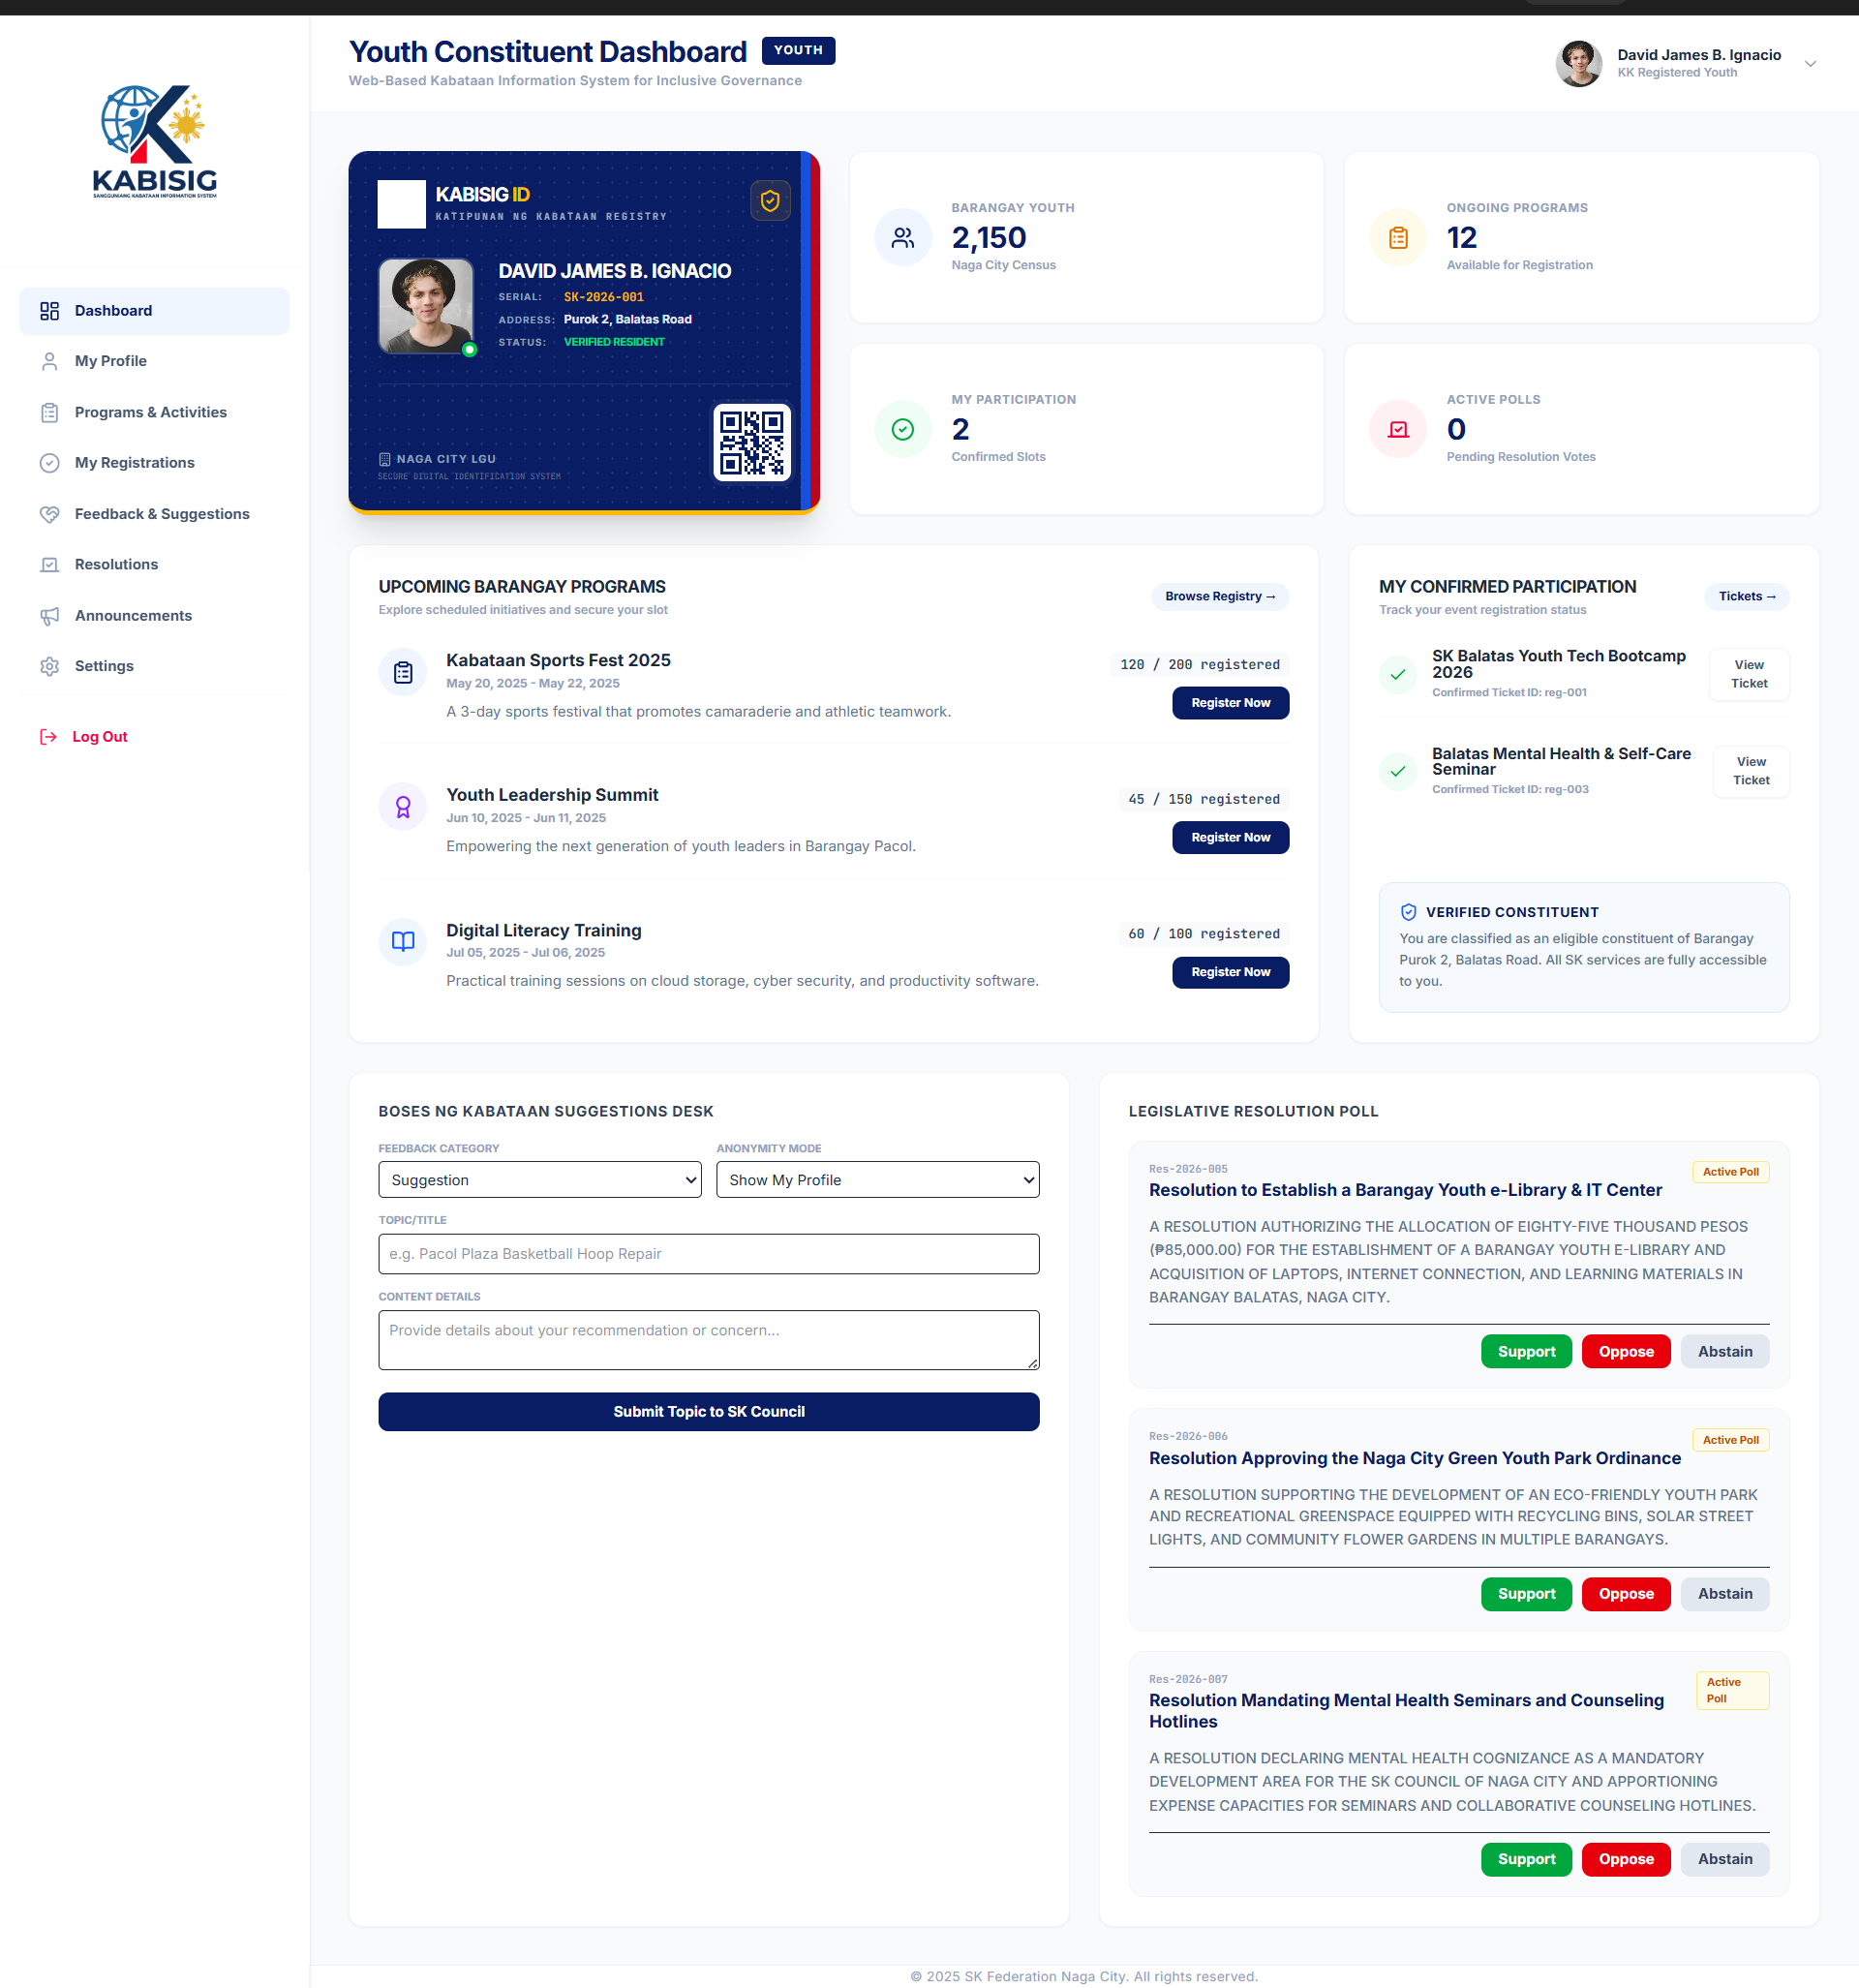
\includegraphics[width=0.45\textwidth]{figures/youth_dashboard.png}
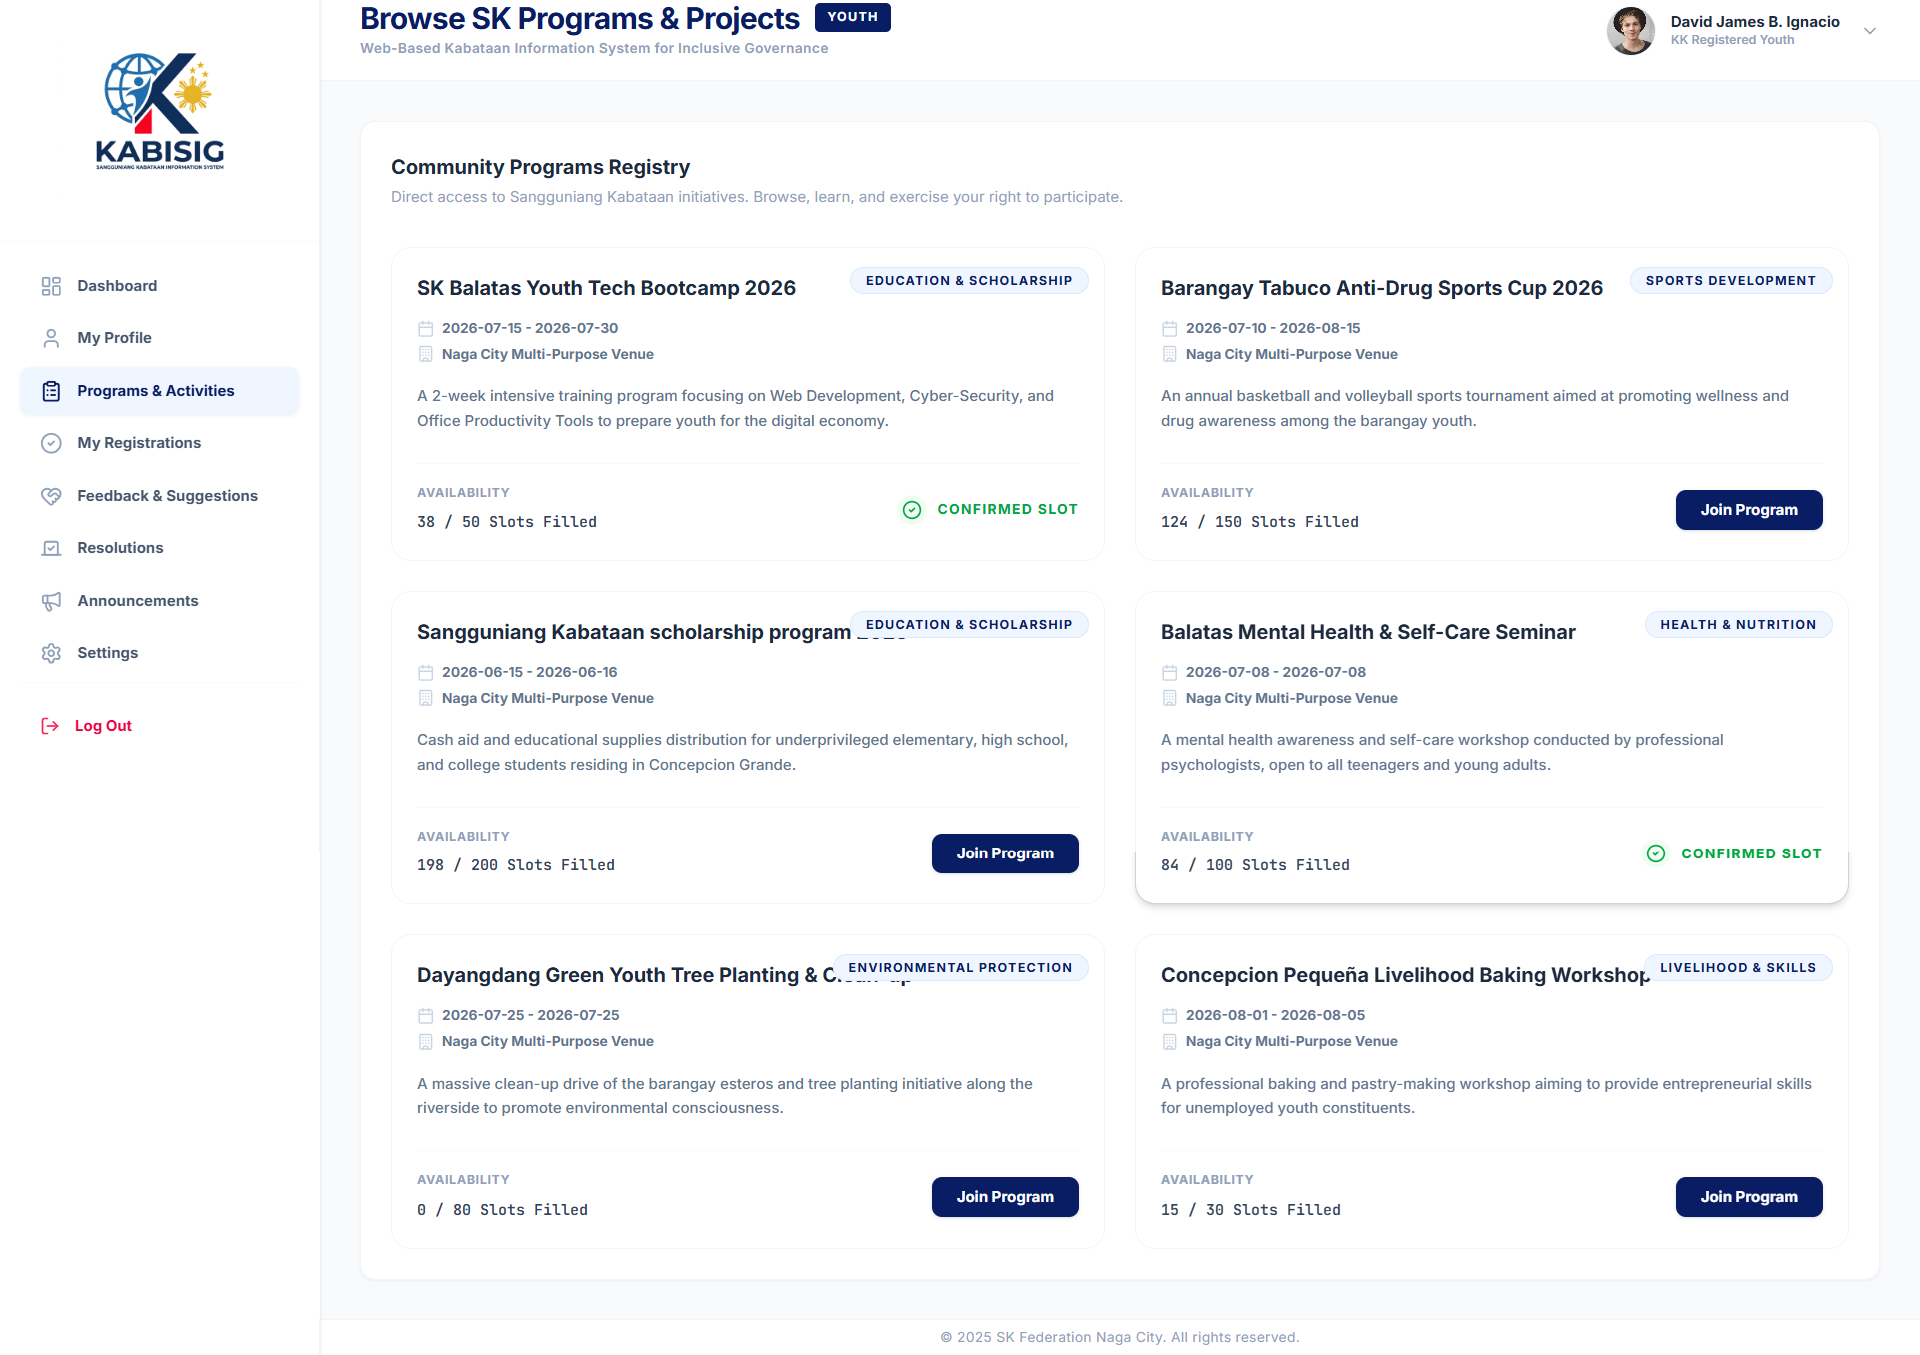
\includegraphics[width=0.45\textwidth]{figures/programs_browse.png}
\caption{Youth Dashboard and Program Browsing Screens (Sample Data)}
\label{fig:youth}
\end{figure}

\hspace*{\parindent} The Browse Programs screen displays available SK programs with details including title, category, date range, location, description, and slot availability. Youth can register for programs with a single click, and confirmed registrations are displayed in the My Confirmed Participation section.\vspace{5mm}

\hspace*{\parindent} The Boses ng Kabataan feedback module allows youth to submit suggestions, concerns, and inquiries to their SK Council. Users can select feedback categories, choose anonymity preferences, and track submission history with status updates and responses from SK officials.\vspace{5mm}

\begin{figure}[H]
\centering
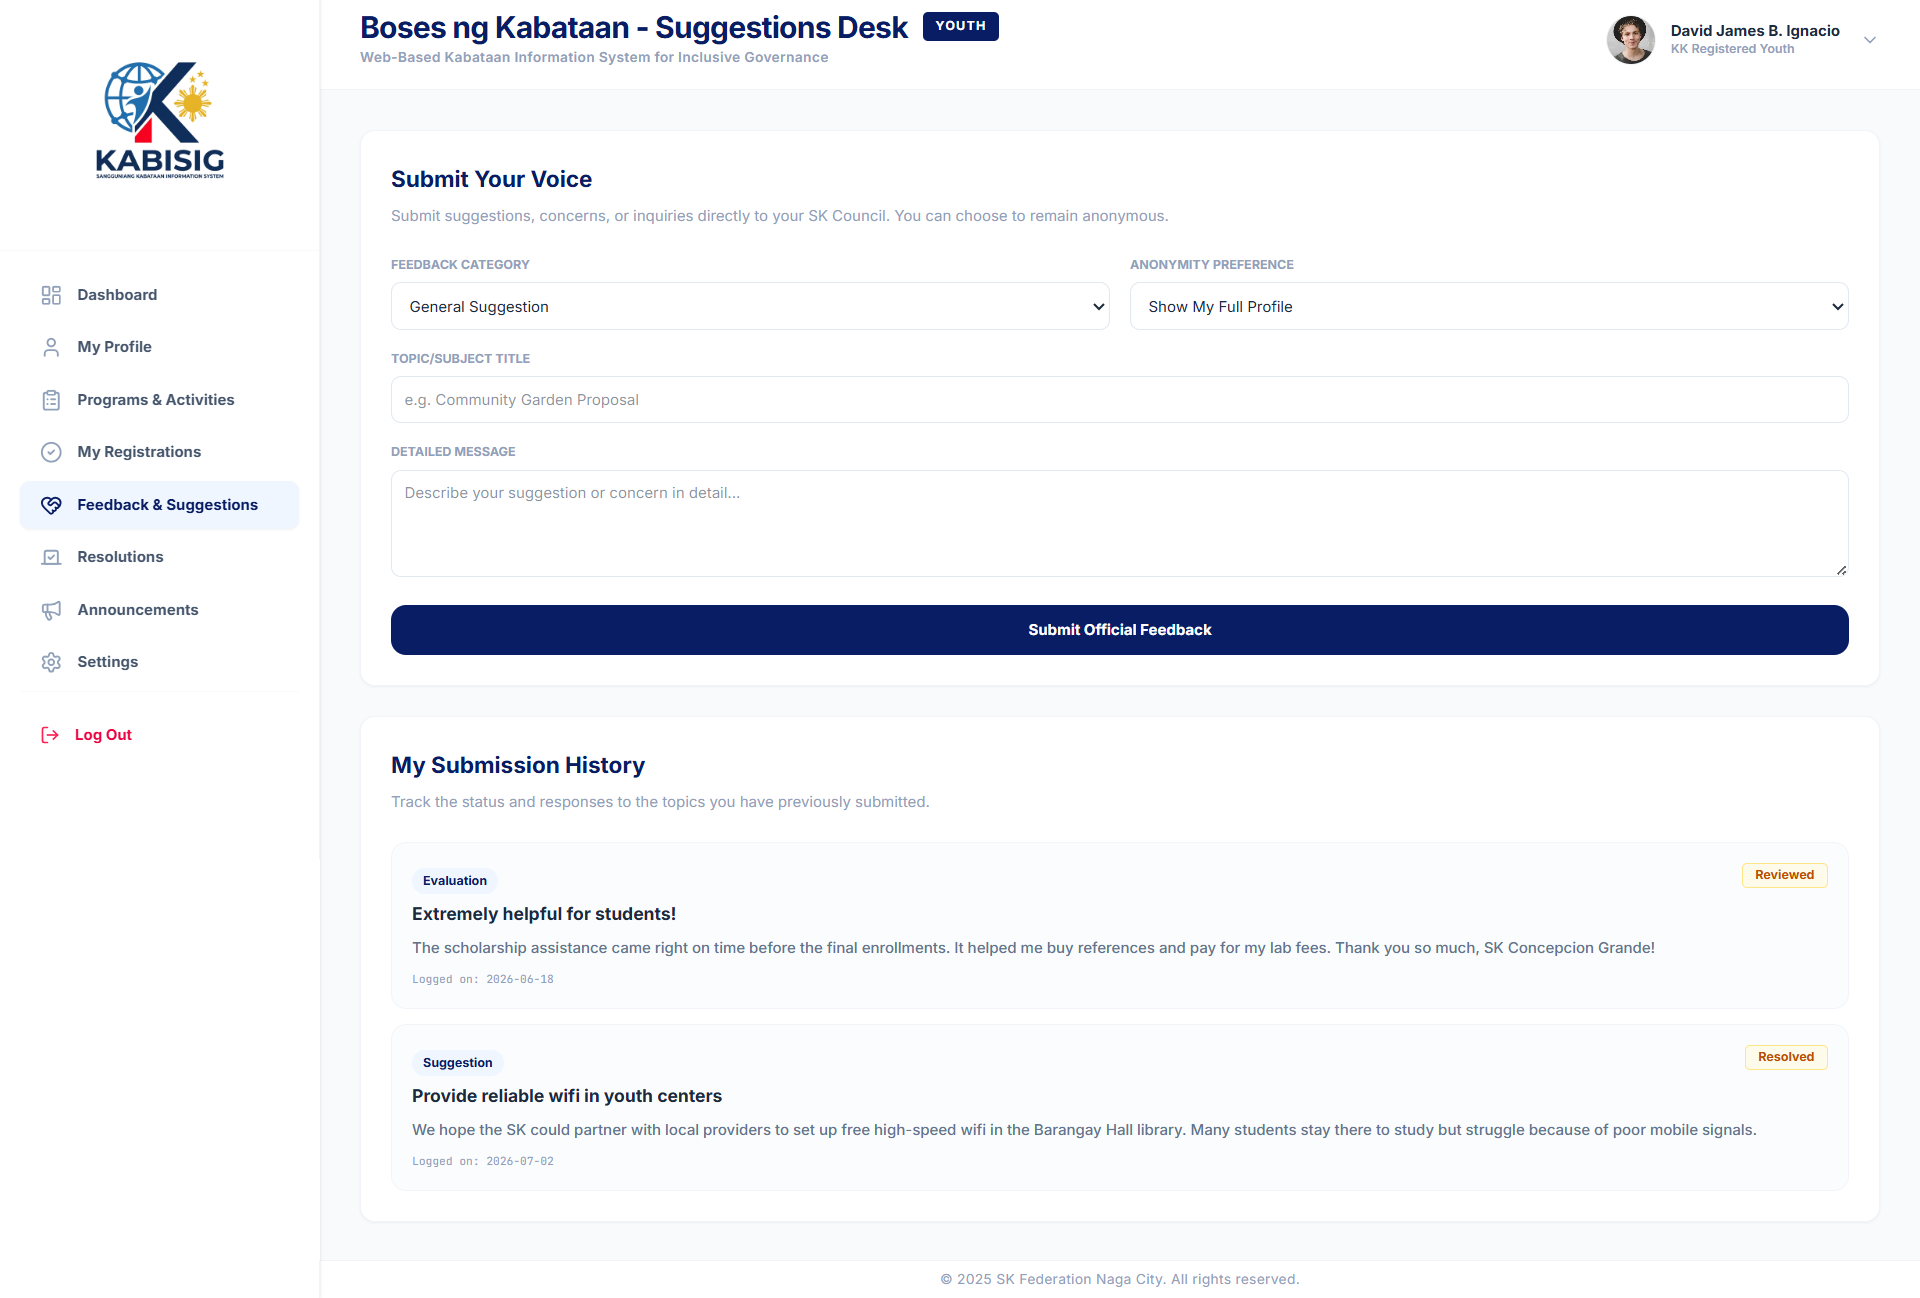
\includegraphics[width=0.45\textwidth]{figures/boses_ng_kabataan.png}
\caption{Boses ng Kabataan Feedback Module (Sample Data)}
\label{fig:feedback}
\end{figure}

\subsubsection{Mobile Responsive Design}

\hspace*{\parindent} All KABISIG screens are designed with a mobile-first approach, ensuring optimal usability on smartphones, tablets, and desktop devices. The interface features touch-friendly elements with minimum 44px touch targets, clear visual hierarchy, and intuitive navigation patterns. Users can efficiently access all system features through any modern web browser without requiring a native application download.\vspace{5mm}

\begin{figure}[H]
\centering
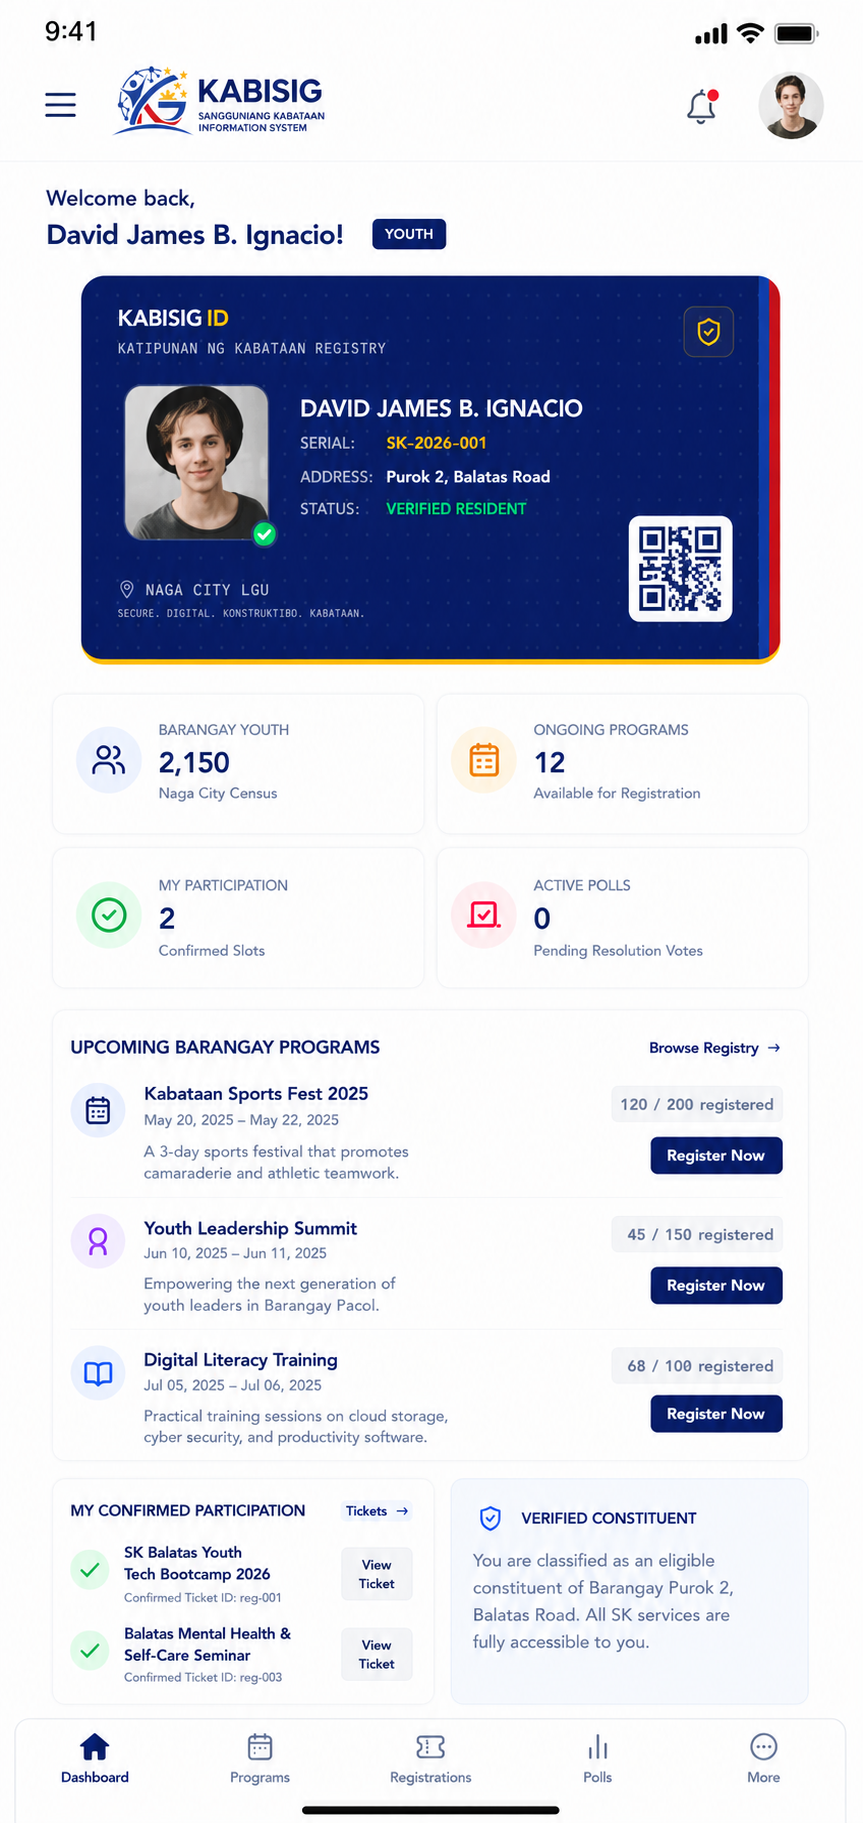
\includegraphics[width=0.30\textwidth]{figures/mobile_dashboard.png}
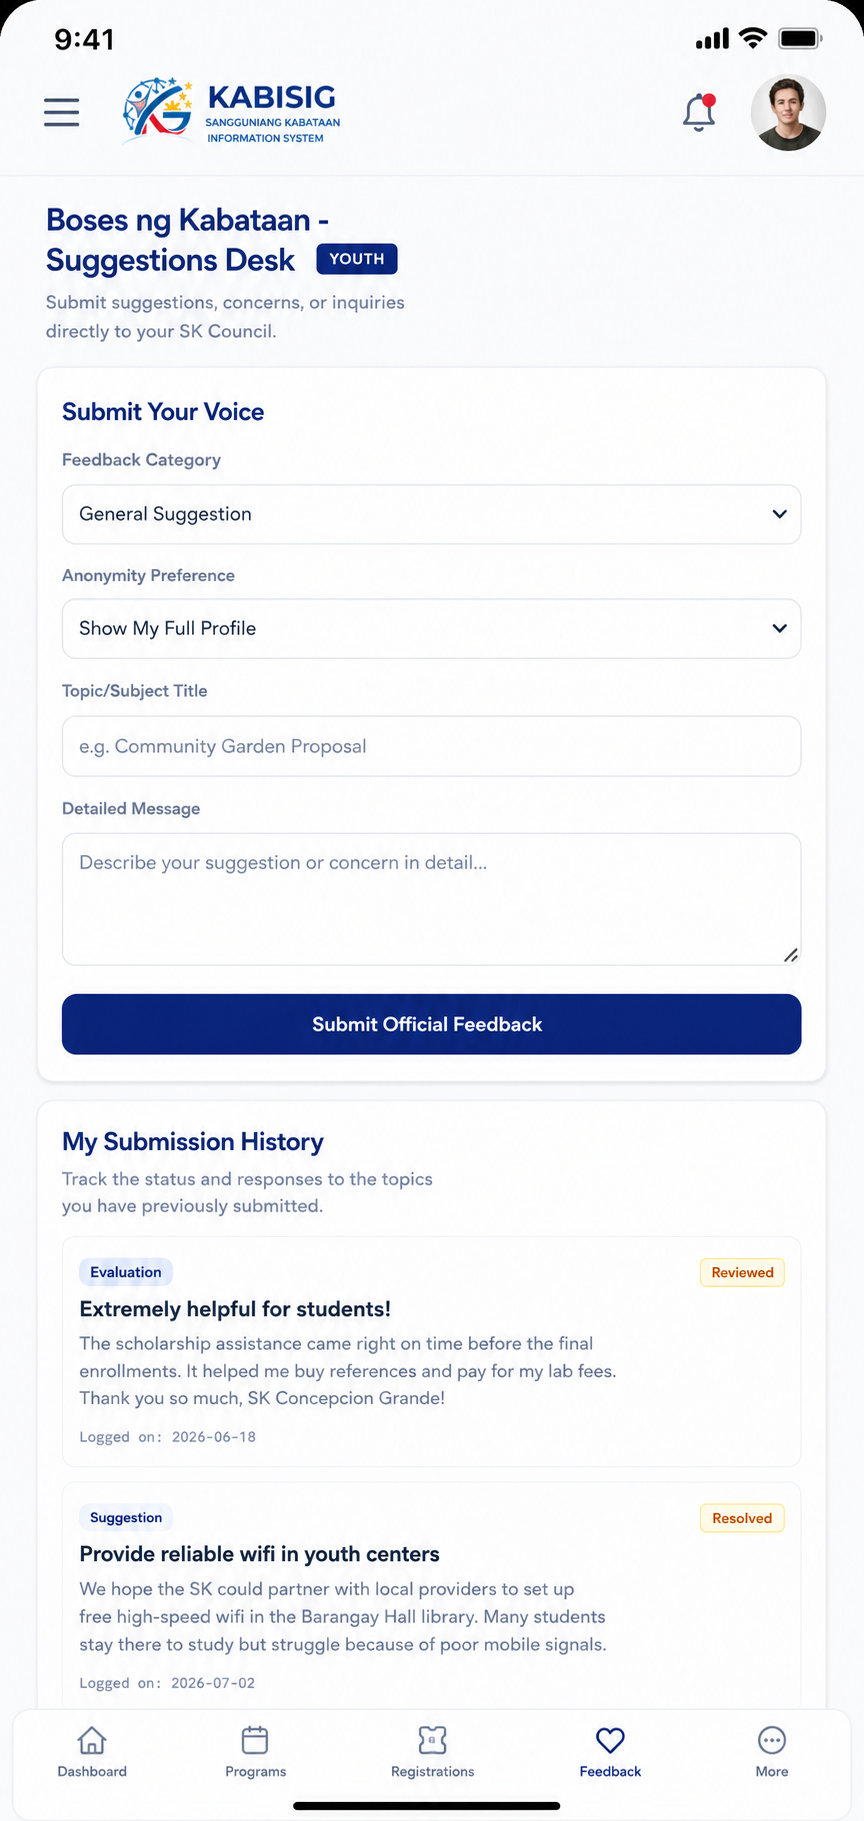
\includegraphics[width=0.30\textwidth]{figures/mobile_feedback.png}
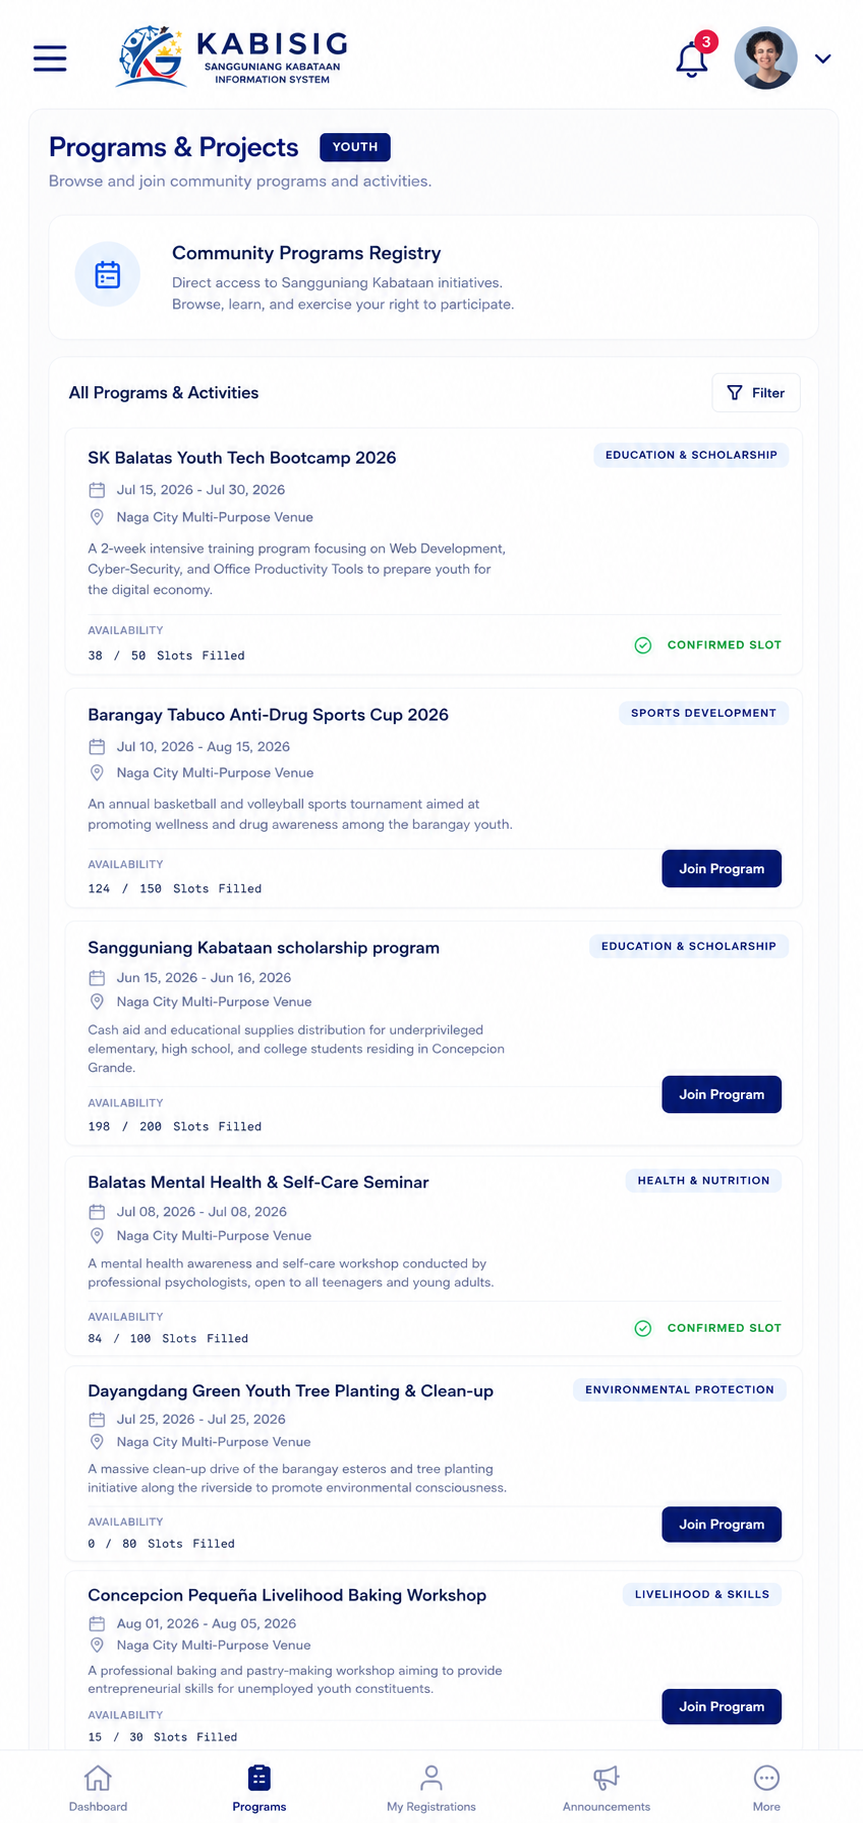
\includegraphics[width=0.30\textwidth]{figures/mobile_program.png}
\caption{Mobile Responsive Views of KABISIG Screens (Sample Data)}
\label{fig:mobile}
\end{figure}

\subsubsection{UI Components and Design System}

\hspace*{\parindent} The KABISIG design system includes reusable UI components that ensure consistency across all screens. These components include:\vspace{3mm}

\begin{itemize}
    \item \textbf{Cards:} White background with 12px border-radius, 16px padding, and subtle shadow for content display
    \item \textbf{Buttons:} Primary (Vibrant Red \#d32f2f), Secondary (Outline), and Text buttons with minimum 48px height for touch targets
    \item \textbf{Input Fields:} Light gray background with 8px border-radius, 14-16px padding, and clear labels
    \item \textbf{Badges:} Color-coded status indicators (Approved: Green, Pending: Yellow, Draft: Gray)
    \item \textbf{Navigation:} Bottom tab bar with icons and labels for mobile; left sidebar for desktop
    \item \textbf{Charts:} Clean, minimalist data visualizations using Recharts and D3.js
\end{itemize}

\vspace{5mm}

\begin{table}[H]
\centering
\caption{KABISIG Design System Color Palette}
\label{tab:colors}
\begin{tabular}{|l|c|l|}
\hline
\textbf{Color Name} & \textbf{Hex Code} & \textbf{Usage} \\
\hline
White & \#ffffff & Backgrounds, cards, text on dark \\
Light Gray & \#f5f5f5 & Section backgrounds, subtle separation \\
Deep Blue & \#1a237e & Headers, titles, primary text, active states \\
Vibrant Red & \#d32f2f & Primary action buttons, alerts, highlights \\
Gold & \#fdd835 & Accents, badges, highlights \\
Dark Text & \#212121 & Body text \\
Medium Text & \#616161 & Secondary text, labels \\
Light Text & \#9e9e9e & Placeholders, hints, subtle text \\
\hline
\end{tabular}
\end{table}

\subsubsection{Navigation Structure}

\hspace*{\parindent} Each user role has a tailored navigation structure that provides access to role-appropriate features and modules. The navigation adapts to screen size: bottom tab bar for mobile devices and left sidebar for tablet and desktop views. Active navigation items are highlighted with the KABISIG brand colors for clear orientation.\vspace{5mm}

\begin{table}[H]
\centering
\caption{KABISIG Navigation by User Role}
\label{tab:navigation}
\begin{tabular}{|>{\centering\arraybackslash}p{2.8cm}|>{\centering\arraybackslash}p{8cm}|}
\hline
\textbf{User Role} & \textbf{Navigation Items} \\
\hline
Super Admin & Dashboard, Barangays, Programs, Reports, More \\
\hline
Barangay Admin & Dashboard, Youth, Programs, Budget, Documents, Reports, Announcements, Social Sync, Calendar, Settings, Profile \\
\hline
SK Kagawad & Dashboard, Programs, Attendance, Resolutions, More \\
\hline
SK Secretary & Dashboard, Documents, Youth, Reports, More \\
\hline
SK Treasurer & Dashboard, Budget, Expenses, Inventory, More \\
\hline
Youth Constituent & Dashboard, Programs, Registrations, Feedback, More \\
\hline
Viewer & Home, Announcements, Transparency, Contact \\
\hline
\end{tabular}
\end{table}

\subsubsection{Accessibility Features}

\hspace*{\parindent} The KABISIG user interface incorporates accessibility features to ensure inclusive access for all users. These include:\vspace{3mm}

\begin{itemize}
    \item \textbf{High Contrast:} Text and background colors meet WCAG contrast ratio requirements
    \item \textbf{Screen Reader Support:} Semantic HTML and ARIA labels for assistive technologies
    \item \textbf{Touch Targets:} Minimum 44px touch targets for all interactive elements
    \item \textbf{Font Sizing:} Responsive typography that scales appropriately across devices
    \item \textbf{Color Blindness Support:} Status indicators use both color and icons for clarity
\end{itemize}

\vspace{5mm}

\hspace*{\parindent} The mobile-responsive design ensures that all KABISIG features remain fully functional and accessible on any device, supporting SK officials and youth constituents in their governance activities anytime, anywhere.\vspace{5mm}


\include{chapters/results}
\include{chapters/recommendations}
% \include{chapters/conclusion} may also be used

\appendix
    
\chapter{Evaluation tool}

\subsection*{Use of Generative AI Tools}

\hspace*{\parindent} The following section details the use of Generative Artificial Intelligence (AI) tools in the course of the development of this project, in accordance with academic integrity policies.

\paragraph{1. Specification of AI-Assisted Components}\hspace*{\parindent} 

\hspace*{\parindent} AI assistance was used for the structuring and preparation of the following parts:
\begin{itemize}
    \item Chapter 1 (Background of the Study): flow organization and grammar improvement.
    \item Chapter 2 (Review of Related Literature and Systems): literature search, system identification and comparison and flow organization.
    \item In-Text and End-Text Citations: cross-referencing, citation formatting and validation.
    \item General Manuscript: grammar improvement and vocabulary improvement.
    \item System Design Documentation: flow organization and specification of modules and features.
    \item KABISIG Logo Design: conceptualization and design refinement of the project logo using ChatGPT.
\end{itemize}

\paragraph{2. Explanation of AI Usage}\hspace*{\parindent} 

\hspace*{\parindent} AI tools were used to enhance the quality, clarity and organization of the manuscript. The AI contribution to Chapter 1 was flow organization and grammar. The AI contribution to Chapter 2 was literature organization and comparison tables development. AI tools helped with consistent cross-referencing, citation formatting and grammar. Additionally, AI was used to generate design concepts and refine the KABISIG logo. Usage of AI tools was restricted only to editorial, organizational, and design purposes. All research conclusions, analyses, interpretations, designs of the system and writing of the manuscript are the intellectual property of the researchers.\vspace{5mm}

\paragraph{3. Justification of Necessity}\hspace*{\parindent} 

\hspace*{\parindent} AI tools were required to increase clarity, cohesion and quality of the manuscript. They helped with organizing of large amount of information in Chapter 2 and consistent citation formatting, thus reducing errors and making possible for researchers to focus more on analysis and design. AI was also used to generate logo concepts, streamlining the design process and providing visual direction for the project's branding.\vspace{5mm}

\paragraph{4. Affirmation of Understanding}\hspace*{\parindent} 

\hspace*{\parindent} The authors recognize, understand and are responsible for all AI-assisted parts in this manuscript. AI tools were used to assist with literature search, organizing of flow, editing, formatting, and logo design. All sources of literature that were found using searches were checked manually. The authors are responsible for all aspects of this work, including originality and integrity of this paper.

    \chapter{Sample Reports}
\subsection*{Figure 1. Resolution Management}

\begin{center}
    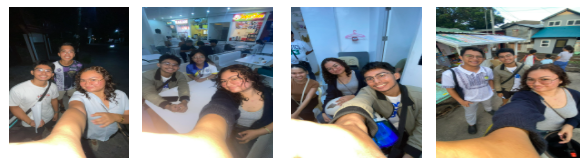
\includegraphics[width=0.75\textwidth]{figures/1.png}
    \par\smallskip
    Resolution Management Screenshot
\end{center}

\noindent
\textbf{Statement 1 by SK Chairman of TABUCO, BALATAS, CONCEPCION GRANDE, DAYANGDANG:}

\hspace*{\parindent}"The resolution tracking feature is very helpful. Before, we had to write resolutions in Word, print them, and it was difficult to track whether they had already been approved. The youth also had no knowledge of our resolutions. With KABISIG, the resolution number is automatically generated and everyone can see the status. The youth can also vote — support or oppose — and there is a validity period so everyone knows how long the resolution remains in effect. This is a great help in making the SK more transparent."\vspace{5mm}


\subsection*{Figure 2. KK Profiling}

\begin{center}
    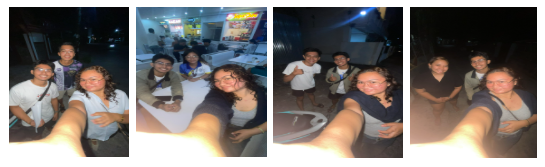
\includegraphics[width=0.75\textwidth]{figures/2.png}
    \par\smallskip
    KK Profiling Screenshot
\end{center}

\noindent
\textbf{Statement 2 by SK Chairman of BALATAS, CONCEPCION GRANDE, TABUCO, DAYANGDANG, IGUALDAD, SAN FELIPE:}

\hspace*{\parindent}"KK profiling should come first before anything else. We need to know the composition of our youth — students, PWDs, registered voters, unemployed, and scholars. Right now, we simply assume what programs are needed. For example, if we see that there are many unemployed youth, we can immediately create a skills training program. With KABISIG, the demographics are visible right away, so we no longer have to guess what programs are appropriate for our community."\vspace{5mm}


\subsection*{Figure 3. Beneficiary Monitoring}

\begin{center}
    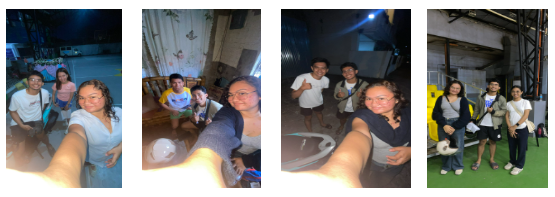
\includegraphics[width=0.75\textwidth]{figures/3.png}
    \par\smallskip
    Beneficiary Monitoring Screenshot
\end{center}

\noindent
\textbf{Statement 3 by SK Chairman of BALATAS, CONCEPCION GRANDE, TABUCO, DAYANGDANG, CONCEPCION PEQUEÑA:}

\hspace*{\parindent}"Our problem is monitoring who is actually being helped. Some youth receive multiple forms of assistance — educational aid, school supplies, and financial aid — while others receive nothing at all. The SK fails to notice this because there is no system in place. With KABISIG, we can see how many programs each youth has already participated in and who has not yet received any benefit. This effectively prevents duplication of assistance and eliminates favoritism."\vspace{5mm}

\subsection*{Figure 4. Budget Transparency}

\begin{center}
    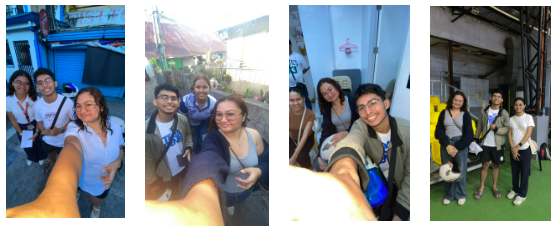
\includegraphics[width=0.75\textwidth]{figures/4.png}
    \par\smallskip
    Budget Transparency Screenshot
\end{center}

\noindent
\textbf{Statement 4 by SK Chairman of TABUCO, DAYANGDANG, CONCEPCION GRANDE, IGUALDAD, BALATAS:}

\hspace*{\parindent}"The public should be able to see the SK's budget — how much was allocated, how much was spent, and how much remains. For example, if the budget for the Basketball League is ₱35,000, everyone can see that ₱30,000 has already been spent and ₱5,000 is still remaining. This increases transparency and builds the community's trust in the SK. The SK's financial records should be open and accessible to everyone."\vspace{5mm}


\subsection*{Figure 5. Automated Budgeting}

\begin{center}
    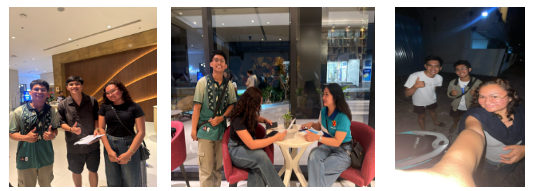
\includegraphics[width=0.75\textwidth]{figures/5.png}
    \par\smallskip
    Automated Budgeting Screenshot
\end{center}

\noindent
\textbf{Statement 5 by SK Chairman of BALATAS, IGUALDAD, CONCEPCION GRANDE, TABUCO, TINAGO:}

\hspace*{\parindent}"Our treasurer is very pleased because the system already has the formulas built in. She no longer needs to manually compute VAT and non-VAT amounts for every transaction. For example, if we purchase a sound system worth ₱10,000, the system automatically computes the VAT, withholding tax, and net payable amount. Before, we relied on Excel which was time-consuming and prone to errors. Now, our budgeting process is far more accurate and much faster."\vspace{5mm}


\subsection*{Figure 6. Document Management}

\begin{center}
    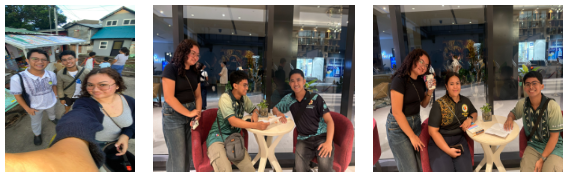
\includegraphics[width=0.75\textwidth]{figures/6.png}
    \par\smallskip
    Document Management Screenshot
\end{center}

\noindent
\textbf{Statement 6 by SK Chairman of TABUCO, DAYANGDANG, CONCEPCION GRANDE, BALATAS, PANICUASON:}

\hspace*{\parindent}"Our documents used to be completely disorganized — piled up in different folders and scattered across Messenger chats. We did not know whether a voucher had already been approved or whether the liquidation was still pending. With KABISIG, all documents are stored in a single repository — resolutions, budget proposals, vouchers, attendance sheets, accomplishment reports, and photos. The status of each document is immediately visible. No more searching through folders and group chats just to find one file."\vspace{5mm}


\subsection*{Figure 7. Notifications \& Announcements}

\begin{center}
    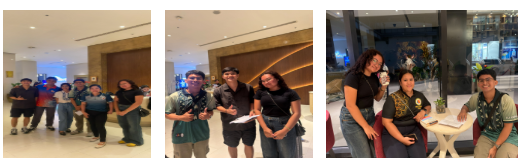
\includegraphics[width=0.75\textwidth]{figures/7.png}
    \par\smallskip
    Notifications \& Announcements Screenshot
\end{center}

\noindent
\textbf{Statement 7 by SK Chairman of PANICUASON, CALAUAG, TABUCO, SAN FELIPE, CONCEPCION PEQUEÑA:}

\hspace*{\parindent}"The notification system is excellent — it sends automated reminders before, during, and after events. For example, for a Clean-Up Drive scheduled on July 15, the system sends a reminder 7 days before, another 1 day before, a reminder on the event day itself, and a follow-up after the event prompting participants to complete the evaluation form. Youth will no longer forget about activities, and they can also provide feedback afterward. This is a great help in improving youth participation and program accountability."\vspace{5mm}


\subsection*{Figure 8. Inventory Management}

\begin{center}
    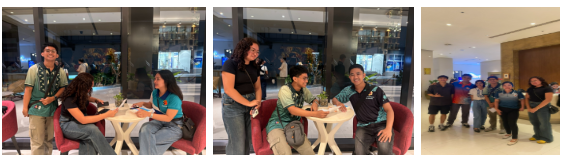
\includegraphics[width=0.75\textwidth]{figures/8.png}
    \par\smallskip
    Inventory Management Screenshot
\end{center}

\noindent
\textbf{Statement 8 by SK Chairman of TABUCO, BALATAS, CONCEPCION GRANDE, IGUALDAD, LIBOTON:}

\hspace*{\parindent}"We need a system to properly track the SK's assets — tables, chairs, speakers, and other equipment. Before, we would lose track of our inventory, especially during the turnover of officers at the end of each SK term. With KABISIG, all assets and their corresponding quantities are properly recorded in the system. When new SK officials take over, an inventory turnover report is automatically generated. Equipment will no longer go missing, and every official is held accountable for the assets under their care."\vspace{5mm}


\subsection*{Figure 9. Official Performance Monitoring}

\begin{center}
    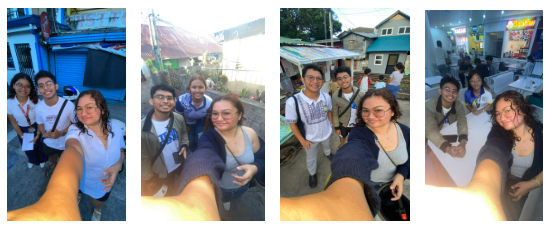
\includegraphics[width=0.75\textwidth]{figures/9.png}
    \par\smallskip
    Official Performance Monitoring Screenshot
\end{center}

\noindent
\textbf{Statement 9 by SK Chairman of IGUALDAD, DAYANGDANG, CONCEPCION GRANDE, BALATAS, SAN FRANCISCO:}

\hspace*{\parindent}"We need to know which SK officials are active and which are not fulfilling their duties. The performance dashboard shows the attendance record of every official. For example, the Secretary has 95\% attendance, the Treasurer has 90\%, but Kagawad A only has 45\%. The Chairperson can immediately identify who is inactive and take the necessary action. This greatly improves accountability within the SK and ensures that every official is properly carrying out their assigned responsibilities."\vspace{5mm}

\subsection*{Figure 10. Feedback \& Rating System}

\begin{center}
    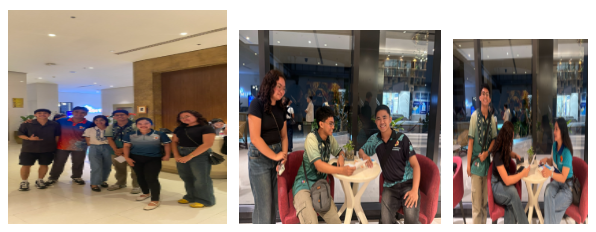
\includegraphics[width=0.75\textwidth]{figures/10.png}
    \par\smallskip
    Feedback \& Rating System Screenshot
\end{center}

\noindent
\textbf{Statement 10 by SK Chairman of TABUCO, SAN FELIPE, CONCEPCION GRANDE, DAYANGDANG, BALATAS:}

\hspace*{\parindent}"The feedback and rating system is excellent because it allows us to gather the actual opinions of the youth about our services. They answer a satisfaction survey — rating how satisfied they are with SK services and how responsive the SK is to their needs. The dashboard then displays each official's rating — for example, the Chairperson at 4.8, the Treasurer at 4.5, and the Secretary at 4.2. This helps us identify which areas and which officials need to improve so that we can provide better service to the community."\vspace{5mm}


\subsection*{Figure 11. Appointment Scheduling}

\begin{center}
    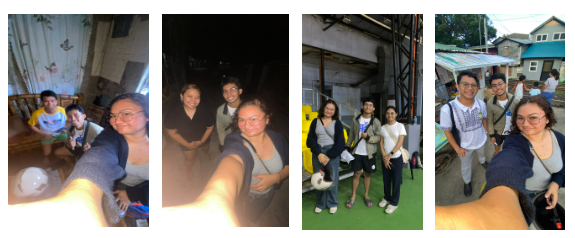
\includegraphics[width=0.75\textwidth]{figures/11.png}
    \par\smallskip
    Appointment Scheduling Screenshot
\end{center}

\noindent
\textbf{Statement 11 by SK Chairman of CONCEPCION GRANDE, PANICUASON, IGUALDAD, CALAUAG, TABUCO:}

\hspace*{\parindent}"Instead of going directly to the barangay hall, youth can now book an appointment online. For example, if they have a scholarship concern, need a certificate, or want to file a complaint, they can schedule a specific date and time with the SK Secretary through the system. They no longer have to waste time waiting at the barangay hall with no guarantee of being attended to. This is very convenient for the youth and ensures that their concerns are addressed in a more organized and timely manner."\vspace{5mm}


\subsection*{Figure 12. Calendar \& Activity Management}

\begin{center}
    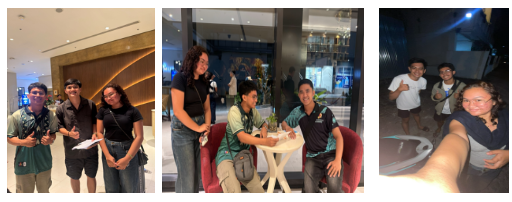
\includegraphics[width=0.75\textwidth]{figures/12.png}
    \par\smallskip
    Calendar \& Activity Management Screenshot
\end{center}

\noindent
\textbf{Statement 12 by SK Chairman of DAYANGDANG, BALATAS, TABUCO, CONCEPCION GRANDE, CALAUAG:}

\hspace*{\parindent}"We need a calendar view of all SK activities — a monthly overview showing event schedules, assigned officials, locations, and related documents. Before, our schedules would conflict and we were unable to properly monitor our activities. With KABISIG, we can immediately see which projects are upcoming, ongoing, and already completed. There is also a historical record of all SK activities, which is very useful for reporting, evaluation, and planning future programs."\vspace{5mm} 


    \include{appendices/io}
    \include{appendices/code}
    \include{appendices/usersguide}


\bibliographystyle{unsrt}
{
\singlespace
\bibliography{references}
}

%%%%%%%%%%%%%%%%%%%%%%%%%%%%%%%%%%%%%%%%%%%%%%%%%%%%%%%%%%%%%%%%%%%%%%%%%%%
% vita.tex -- Authors Page
%%%%%%%%%%%%%%%%%%%%%%%%%%%%%%%%%%%%%%%%%%%%%%%%%%%%%%%%%%%%%%%%%%%%%%%%%%%

\thispagestyle{empty}          % no page number, if desired
\vspace*{\fill}                % push content toward vertical center

\begin{center}
{\large\bfseries VITA}\\[1.5em]

Ashley Kyla D. Vinzon is a BS Information Technology student of the Department of Computer Science\\
at the Ateneo de Naga University.\\[1em]

David James B. Ignacio is a BS Information Technology student of the Department of Computer Science\\
at the Ateneo de Naga University.\\[2em]

{\large\bfseries End of Manuscript}
\end{center}

\vspace*{\fill}
\newpage

\end{document}
